\documentclass[12pt,a4paper]{article}

% --- Packages ---
\usepackage[margin=2.5cm]{geometry}
\usepackage{graphicx}
\usepackage{booktabs}
\usepackage{tabularx}
\usepackage{amsmath}
\usepackage{amssymb}
\usepackage{hyperref}
\usepackage{caption}
\usepackage{subcaption}
\usepackage{float}
\usepackage{enumitem}
\usepackage{longtable}
\usepackage{xcolor}
\usepackage{natbib}
\usepackage{microtype}
\usepackage{setspace}
\usepackage{tikz}
\usepackage{array}
\usetikzlibrary{shapes.geometric,arrows.meta,positioning}

% --- Fix: define C column type for tabularx ---
\newcolumntype{C}{>{\centering\arraybackslash}X}

% --- Document Formatting ---
\onehalfspacing
\hypersetup{
    colorlinks=false,
    pdfborder={0 0 0},
    pdftitle={Adversarial Cognition Divergence},
    pdfauthor={Mina Magdy, Sandy Antonius, Youssef Tammam Mahmoud, Eyad Saleh Ali, Mariam Mohammed}
}

\title{\textbf{Adversarial Cognition Divergence: Mapping Perceptual Breakdown\\
Across Neural Architectures and Human Vision}}

\author{
    Mina Magdy\textsuperscript{1} \quad
    Sandy Antonius\textsuperscript{1} \quad
    Youssef Tammam Mahmoud\textsuperscript{1} \\[4pt]
    Eyad Saleh Ali\textsuperscript{1} \quad
    Mariam Mohammed\textsuperscript{1} \\[8pt]
    \small\textsuperscript{1}Sadat Academy for Management Sciences,
    AI Department, Year~3
}

\date{\small\today}

\begin{document}

\maketitle
\thispagestyle{empty}

% ============================================================
\begin{abstract}
% ============================================================
Deep neural networks achieve superhuman performance on clean visual datasets
yet exhibit extreme vulnerability to adversarial perturbations --- a
qualitative divergence from biological vision that remains poorly understood.
This study presents the \textit{Adversarial Cognition Divergence} (ACD)
project: a systematic, cross-disciplinary effort to measure, understand,
and close the gap between human and machine perceptual robustness.

We evaluate seven neural architectures spanning the full
locality-to-globality processing spectrum --- BagNet-33, ResNet-18,
EfficientNet-B0, Shape-ResNet-50, CORnet-S, ViT-Small, and our proposed
\textit{Recurrent Hybrid Attention Network} (RHAN) --- against human
observers ($n{=}18$, 1\,800 psychophysical trials) under identical
adversarial constraints. Using Signal Detection Theory (SDT) as a
scale-invariant comparison framework, we measure perceptual sensitivity
($d'$) and collapse thresholds ($\varepsilon_{\text{thresh}}$) across
all systems.

All standard feedforward architectures collapse below the
reliable-discrimination threshold ($d'{<}1.0$) before
$\varepsilon{=}0.031$, while human sensitivity remains stable
($d'{=}2.019$) at $\varepsilon{=}0.30$ --- a ten-fold gap.
EfficientNet-B0 is the most fragile model despite the highest clean
accuracy ($\varepsilon_{\text{thresh}}{=}0.0062$); ResNet-18 is
paradoxically the most robust standard architecture
($\varepsilon_{\text{thresh}}{=}0.0295$). Shape-biased training via
Stylized-ImageNet fails to improve over the standard texture-biased
baseline, constituting a negative result that challenges the sufficiency
of texture-bias explanations for adversarial fragility.

Our proposed RHAN, combining local convolutional smoothing, global
self-attention, and recurrent top-down feedback trained via curriculum
adversarial training, achieves $\varepsilon_{\text{thresh}}{=}0.1850$
on CIFAR-10 --- a 6.3$\times$ improvement over ResNet-18 and
29$\times$ over EfficientNet-B0. To test whether higher input
resolution further closes the gap, we train and evaluate RHAN on STL-10
($96{\times}96$), finding that both car and truck classes collapse to
0\% under AutoAttack at $\varepsilon{=}0.031$, suggesting that
resolution alone is insufficient without the right architectural
inductive biases.

We conclude that biological-like recurrent feedback, rather than
feedforward scaling, shape-biased training, or resolution increases,
is the primary mechanism for closing the human-machine robustness gap
--- but that fully closing it likely requires combining recurrence with
language-grounded semantic representations.
\end{abstract}

\newpage
\tableofcontents
\newpage

% ============================================================
\section{Introduction}
\label{sec:intro}
% ============================================================

There is a moment --- and anyone who has seen it knows the feeling ---
where a deep neural network goes from seeming infidelity to utter
absurdity. A panda becomes a gibbon. A school bus becomes an ostrich.
A 3D-printed turtle becomes a rifle. The changes are invisible to the
human eye. The network's confidence is absolute. And somewhere in the
gap between what the machine sees and what we see lies one of the most
important unsolved problems in artificial intelligence: \textit{why are
machines so easily fooled?}

This is not merely an engineering inconvenience. It is a window into
something deeper --- a fundamental qualitative divergence between how
biological and artificial visual systems process the world. Human vision
has been shaped by hundreds of millions of years of evolution to be
robust: we recognize objects in fog, in dim light, in clutter, under
occlusion, and under the kind of systematic corruption that would
cripple any state-of-the-art classifier. A child can recognize a cat
whether it is photographed, painted, drawn in crayon, or glimpsed
through a rain-streaked window. No current AI system comes close to
this kind of flexible, robust generalization.

The divergence becomes stark under \textit{adversarial perturbations}:
small, carefully crafted changes to an image that are imperceptible to
humans but cause machine classifiers to fail catastrophically with high
confidence. First identified by \citet{szegedy2013intriguing}, these
adversarial examples have proven remarkably difficult to defend against.
The Fast Gradient Sign Method (FGSM) \citep{goodfellow2015explaining}
showed that even a single step of gradient-based perturbation could
fool deep networks. Projected Gradient Descent (PGD)
\citep{madry2018towards} extended this to a multi-step iterative attack
that remains the standard first-order threat model. The Carlini-Wagner
(C\&W) attack \citep{carlini2017towards} showed that even
optimization-based minimum-distortion attacks could find adversarial
examples that are truly invisible to human observers.

But here is the puzzle that motivates our work: \textit{why} are
feedforward architectures so fragile? And more importantly: \textit{what
would it take to build a machine that sees more like we do?}

\subsection{The Biological Gap}

The answer, we believe, lies in the architecture of biological vision
itself. The primate visual system is not a feedforward pipeline. The
initial sweep through the ventral pathway
(V1$\to$V2$\to$V4$\to$IT) is immediately followed by massive
top-down recurrent feedback connections
\citep{dicarlo2007untangling} that allow the visual cortex to apply
contextual predictions, reconstruct degraded signals, and integrate
global shape structure under high-noise conditions. These recurrent
loops are not optional embellishments --- they are the primary
computational mechanism by which biological vision achieves its
remarkable robustness.

Standard deep neural networks, by contrast, are almost entirely
feedforward. They rely heavily on local high-frequency texture
statistics rather than global shape integration
\citep{geirhos2019imagenet,brendel2019approximating}. Adversarial
perturbations exploit this texture bias by injecting high-frequency
patterns that override clean local features while leaving global shape
intact for human observers. The result is a systematic failure mode
that has no analogue in biological vision.

\subsection{Our Approach}

This paper presents the \textit{Adversarial Cognition Divergence} (ACD)
project: a rigorous, cross-disciplinary study that measures the
perceptual breakdown of biological and machine vision under identical
adversarial constraints. Our approach is distinguished by several key
design choices:

\textbf{Architectural spectrum.} We evaluate seven models spanning the
full locality-to-globality range: from BagNet-33 (which classifies using
only $33{\times}33$ pixel local patches, with zero global context) to
ViT-Small (which uses global self-attention from the first layer). This
spectrum lets us isolate the contribution of each architectural
principle to robustness.

\textbf{Human psychophysics.} We collect data from 18 human observers
(1\,800 trials) performing a 10-alternative forced-choice
classification task under the same PGD perturbations used to attack the
machines. This provides a direct, apples-to-apples comparison.

\textbf{Signal Detection Theory.} We use SDT \citep{green1966signal}
as our primary comparison framework. Unlike raw accuracy, $d'$ is
scale-invariant and abstracts away differences in logits and confidence
scores, providing a mathematically principled measure of perceptual
sensitivity that can be compared across biological and artificial
systems on equal footing.

\textbf{Cross-dataset evaluation.} We evaluate on both CIFAR-10
($32{\times}32$) and STL-10 ($96{\times}96$) to test whether higher
resolution alone can close the robustness gap.

\textbf{A proposed architecture.} We introduce the \textit{Recurrent
Hybrid Attention Network} (RHAN), a biologically motivated architecture
that combines local convolutional smoothing, global transformer
attention, and recurrent top-down feedback --- trained via a novel
curriculum adversarial training procedure.

\subsection*{Contributions}

\begin{enumerate}[leftmargin=1.5em]
  \item A large-scale psychophysical study ($n{=}18$, 1\,800 trials)
        measuring human object recognition accuracy and confidence under
        PGD perturbations at six epsilon levels.
  \item A systematic SDT comparison of seven architectures spanning
        the full locality-to-globality spectrum, measuring $d'$ decay
        curves and precise collapse thresholds.
  \item A \textbf{ResNet paradox}: clean-accuracy scaling (EfficientNet)
        produces the most fragile model; the simplest architecture
        (ResNet-18) is the most robust standard model.
  \item A \textbf{negative result for shape-biased training}:
        Shape-ResNet-50 performs worse than standard ResNet-18 under
        adversarial attack despite explicit texture debiasing.
  \item A \textbf{negative result for resolution}: STL-10 ($96{\times}96$)
        evaluation shows both car and truck classes collapse to 0\% under
        AutoAttack, suggesting resolution alone is insufficient.
  \item The \textbf{Recurrent Hybrid Attention Network (RHAN)}, a family of
        biologically motivated architectures combining local convolutional
        smoothing, global self-attention, and recurrent top-down feedback.
        Our best variant, RHAN-trades-curriculum, achieves
        $\varepsilon_{\text{thresh}}{=}0.1850$ on CIFAR-10 ---
        a 6.3$\times$ improvement over ResNet-18 and 29$\times$ over
        EfficientNet-B0. The full RHAN trajectory (RHAN-clean → RHAN-adv
        → RHAN-v5-TRADES → RHAN-TRADES-Hardened → RHAN-trades-curriculum)
        demonstrates progressive closure of the human-machine gap.
  \item A \textbf{confidence-accuracy dissociation} analysis showing
        that all standard models maintain near-maximum confidence even
        as accuracy collapses to zero, while human confidence tracks
        actual perceptual difficulty.
\end{enumerate}

% ============================================================
\section{Related Work}
\label{sec:related}
% ============================================================

The study of adversarial robustness has produced a rich body of work
across attack methodologies, defense strategies, and theoretical
analyses. We organize the relevant literature along three axes:
attack methods, architectural comparisons, and human-machine studies.

\subsection{Adversarial Attack Methods}

Adversarial examples were first identified by
\citet{szegedy2013intriguing}, who showed that deep networks could be
fooled by imperceptible perturbations found through constrained
optimization. \citet{goodfellow2015explaining} proposed the Fast
Gradient Sign Method (FGSM), framing vulnerability as a consequence of
high-dimensional linearity and showing that a single step of signed
gradient perturbation was sufficient to cause misclassification.

\citet{madry2018towards} extended this to Projected Gradient Descent
(PGD), which iteratively takes small steps in the gradient direction
and projects back onto the $\varepsilon$-ball after each step. PGD
remains the standard first-order adversarial threat model and is
considered the strongest attack when given sufficient steps.
\citet{croce2020reliable} introduced AutoAttack, an ensemble of
parameter-free attacks (APGD-CE, APGD-T, FAB-T, and SQUARE) that
provides a more reliable robustness estimate than PGD alone by
mitigating gradient masking.

\citet{carlini2017towards} introduced the C\&W attack, an
optimization-based approach that minimizes $L_2$ perturbation
subject to a misclassification constraint. This produces
minimum-distortion adversarial examples that are directly analogous
to psychophysical just-noticeable-difference (JND) thresholds.

\subsection{Architectural Comparisons}

The texture-bias hypothesis was formalized by
\citet{geirhos2019imagenet}, who demonstrated that ImageNet-trained
CNNs classify by local texture while humans classify by global shape.
They showed that training on Stylized-ImageNet (SIN), where textures
are replaced by neural style transfer, could shift the bias toward
shape-based processing.

\citet{brendel2019approximating} showed that BagNet, restricted to
$33{\times}33$ pixel local patches, achieves surprisingly high
ImageNet accuracy, proving that global context is not required for
feedforward clean performance. This raises the question: if global
context isn't needed for clean accuracy, is it needed for robustness?

\citet{dosovitskiy2020image} introduced the Vision Transformer (ViT),
replacing local convolutions with global patch-level self-attention.
ViT achieves state-of-the-art clean accuracy but its adversarial
robustness properties are less well understood.

\citet{kubilius2019brain} developed CORnet-S, a shallow recurrent
network modeling primate visual areas V1$\to$V2$\to$V4$\to$IT with
recurrent feedback within each stage. CORnet-S achieves high brain-score
alignment but its adversarial robustness has not been systematically
evaluated.

\subsection{Human-Machine Comparison}

\citet{elsayed2018adversarial} conducted a pioneering study comparing
human and machine vision under adversarial perturbations, finding that
human accuracy remains stable at perturbation levels that completely
destroy machine performance. However, their study used a limited set of
architectures and did not apply SDT analysis.

\citet{zhou2020hiring} compared human and machine attention patterns
using eye-tracking, finding that human fixations are more robust to
adversarial perturbations than machine attention maps.

Despite these advances, no prior study has applied SDT across a
comprehensive architectural spectrum while simultaneously collecting
human psychophysical data on identical adversarial stimuli. Our work
fills this gap.

% ============================================================
\section{Methods}
\label{sec:methods}
% ============================================================

\subsection{Datasets}

\textbf{CIFAR-10} \citep{krizhevsky2009learning} serves as our primary
benchmark: 60\,000 RGB images ($32{\times}32$ pixels) across 10 balanced
classes (airplane, automobile, bird, cat, deer, dog, frog, horse, ship,
truck), with 50\,000 training and 10\,000 test images. The standard test
split is used for all adversarial evaluation. Images are normalized using
CIFAR-10 channel statistics:
$\mu{=}(0.4914,\,0.4822,\,0.4465)$,
$\sigma{=}(0.2023,\,0.1994,\,0.2010)$.
A pixel-space validity clamp is applied after all perturbations.

\textbf{STL-10} serves as our high-resolution extension: 13\,000 labeled
RGB images ($96{\times}96$ pixels) across 10 classes (airplane, bird,
car, cat, deer, dog, horse, monkey, ship, truck), with 5\,000 training
and 8\,000 test images. STL-10 provides 9$\times$ more pixels per image
than CIFAR-10, allowing us to test whether increased spatial resolution
alone can close the robustness gap. Images are normalized using STL-10
channel statistics:
$\mu{=}(0.4467,\,0.4398,\,0.4066)$,
$\sigma{=}(0.2242,\,0.2215,\,0.2239)$.

Models requiring larger inputs (EfficientNet-B0, ViT-Small,
Shape-ResNet-50, CORnet-S, RHAN) receive CIFAR-10 images upsampled to
$224{\times}224$ via bilinear interpolation. STL-10 models receive
native $96{\times}96$ inputs.

\subsection{Model Architectures}

We evaluate seven models spanning the locality-to-globality spectrum
(Figure~\ref{fig:architecture_spectrum}):

\begin{enumerate}[leftmargin=1.5em]

  \item \textbf{BagNet-33} \citep{brendel2019approximating}.
        Classifies using only $33{\times}33$ pixel local patches
        extracted at multiple scales and aggregated by max-pooling.
        Represents maximum texture bias with zero global context.
        Clean accuracy: \textbf{87.7\%}.

  \item \textbf{ResNet-18} \citep{he2016deep}.
        Standard 18-layer residual CNN with skip connections.
        ImageNet pretrained, fine-tuned on CIFAR-10 using SGD with
        momentum and CosineAnnealingLR (50 epochs, $\text{lr}{=}0.01$).
        Clean accuracy: \textbf{95.8\%}.

  \item \textbf{EfficientNet-B0} \citep{tan2019efficientnet}.
        Compound-scaled CNN optimizing depth, width, and resolution
        simultaneously via neural architecture search. Uses Swish
        activation and squeeze-and-excitation blocks. Due to gradient
        instability in Swish and BatchNorm layers at
        $224{\times}224$ under high-$\varepsilon$ PGD, BIM (PGD
        without random start) is used for attack generation.
        Clean accuracy: \textbf{96.8\%}.

  \item \textbf{Shape-ResNet-50} \citep{geirhos2019imagenet}.
        ResNet-50 pretrained on Stylized-ImageNet (SIN), where
        textures are replaced by neural style transfer, forcing
        shape-based processing. Fine-tuned on CIFAR-10 (15 epochs,
        $\text{lr}{=}0.0001$). Clean accuracy: \textbf{91.5\%}.

  \item \textbf{CORnet-S} \citep{kubilius2019brain}.
        Shallow recurrent network modeling primate visual areas
        V1$\to$V2$\to$V4$\to$IT with recurrent feedback within each
        stage. Designed for brain-score alignment. ImageNet pretrained,
        fine-tuned on CIFAR-10. Clean accuracy: \textbf{91.5\%}.

  \item \textbf{ViT-Small} \citep{dosovitskiy2020image}.
        Vision Transformer with $16{\times}16$ patch tokenization,
        global self-attention from the first layer. ImageNet pretrained
        via \texttt{timm}, fine-tuned with AdamW and
        CosineAnnealingLR. Clean accuracy: \textbf{97.8\%}.

  \item \textbf{RHAN (Recurrent Hybrid Attention Network)} (proposed).
        Our architecture combining a local convolutional stem, global
        transformer attention layers, and a recurrent top-down feedback
        gate (Section~\ref{sec:rhan_arch}). Five variants spanning the
        robustness trajectory: RHAN-clean (89.1\%), RHAN-adv (83.8\%,
        30-epoch curriculum), RHAN-v5-TRADES (87.3\%, TRADES loss),
        RHAN-TRADES-Hardened (86.3\%, class-hardened fine-tuning), and
        RHAN-trades-curriculum (78.1\%, 60-epoch 3-phase TRADES
        curriculum, $\varepsilon$ from 0.062 to 0.150).

\end{enumerate}

\subsection{Adversarial Attacks}

\textbf{FGSM} \citep{goodfellow2015explaining}.
Single-step signed-gradient attack:
$\mathbf{x}_{\text{adv}} = \mathbf{x} +
\varepsilon \cdot \operatorname{sign}(\nabla_{\!\mathbf{x}}
J(\theta,\mathbf{x},y))$.

\textbf{PGD-$k$} \citep{madry2018towards}.
Iterative multi-step attack with $k$ steps:
\begin{equation}
  \mathbf{x}^{t+1} = \Pi_{\varepsilon}\!\left(
    \mathbf{x}^{t} +
    \alpha\cdot\operatorname{sign}(\nabla_{\!\mathbf{x}} J)
  \right), \qquad \alpha = \varepsilon/4.
  \label{eq:pgd}
\end{equation}
Random initialization within the $\varepsilon$-ball is used for all
models except EfficientNet-B0 (BIM mode without random start). We use
PGD-100 as our primary evaluation attack and PGD-20 for efficient
sweeps.

\textbf{AutoAttack} \citep{croce2020reliable}.
An ensemble of four parameter-free attacks: APGD-CE (cross-entropy),
APGD-T (targeted), FAB-T (fast adaptive boundary), and SQUARE (random
search). AutoAttack provides a more reliable robustness estimate than
PGD alone by mitigating gradient masking. We use the standard version
with $\varepsilon{=}0.031$.

\textbf{C\&W $L_2$} \citep{carlini2017towards}.
Optimization-based attack minimizing $L_2$ perturbation distance
subject to misclassification. Applied to ResNet-18 for supplementary
analysis.

Attacks are evaluated at
$\varepsilon \in \{0.00, 0.01, 0.05, 0.10, 0.20, 0.30\}$
in normalized pixel space.

\subsection{RHAN Architecture}
\label{sec:rhan_arch}

The Recurrent Hybrid Attention Network (RHAN) is designed to
incorporate three processing principles inspired by biological vision:

\textbf{(1) Local convolutional stem.} A four-layer convolutional stem
with residual connections extracts locally smoothed features. The
convolutional layers act as spatial low-pass filters that attenuate
high-frequency adversarial noise (Regime-1 smoothing). For CIFAR-10
($32{\times}32$), the stem produces a $8{\times}8$ feature map with
512 channels (64 spatial tokens). For STL-10 ($96{\times}96$), the stem
produces a $12{\times}12$ feature map with 512 channels (144 spatial
tokens).

\textbf{(2) Global transformer attention.} A 3-layer transformer with
8-head self-attention processes the tokenized feature map, enabling
global integration of spatial information (Regime-2 shape integration).
The transformer uses pre-norm architecture with GELU activation and
a 2048-dimensional feedforward hidden layer.

\textbf{(3) Recurrent top-down feedback.} After the transformer
produces its output, a feedback pathway routes global information back
to the convolutional stem through a learned gating mechanism. A
$1{\times}1$ convolutional network with sigmoid activation produces
a gating map $g \in [0,1]$ that modulates the stem features:
$\mathbf{f}_{\text{modulated}} = \mathbf{f}_{\text{stem}} + g \cdot \mathbf{f}_{\text{feedback}}$.
This loop runs for 2 recurrent steps during inference, implementing
a top-down feedback mechanism analogous to the recurrent connections
in the primate ventral stream.

The classification head uses a cosine similarity projection
(SemanticProjectionHead) rather than a standard linear layer, which
creates a more structured decision boundary in the embedding space.
We found empirically that replacing the cosine head with a linear head
causes clean accuracy to collapse from ~73\% to ~13\%.

\subsection{RHAN Curriculum Adversarial Training}

RHAN-adv is trained in three progressive stages starting from the
RHAN-clean checkpoint:

\begin{itemize}[leftmargin=1.5em]
  \item \textbf{Stage 1} (epochs 1--10): PGD-5, $\varepsilon{=}0.031$
        (8/255). Introduces the model to adversarial examples at a
        low perturbation level.
  \item \textbf{Stage 2} (epochs 11--20): PGD-5, $\varepsilon{=}0.062$
        (16/255). Increases perturbation strength once the model has
        learned initial adversarial features.
  \item \textbf{Stage 3} (epochs 21--30): PGD-5, $\varepsilon{=}0.100$
        (26/255). Final hardening at the target perturbation level.
\end{itemize}

Each stage uses 50\% adversarial + 50\% clean mixed batches (effective
batch size 128), AdamW ($\text{lr}{=}5{\times}10^{-5}$, weight decay
0.05), and CosineAnnealingLR. The model is saved at the final epoch
regardless of clean accuracy, ensuring the fully hardened weights are
preserved.

\subsection{Human Psychophysics Study}

Eighteen university students (age range 19--22, normal or
normal-to-corrected vision) participated voluntarily. Stimuli were
PGD-perturbed images generated against ResNet-18, upscaled to
$128{\times}128$ using nearest-neighbour interpolation to make
perturbations visible on screen.

A stratified sample of 100 images (10 per class) was selected at each
of 6 epsilon levels using fixed random seed 42, yielding 600 unique
stimuli. Each participant viewed a random subset of 30 stimuli per
epsilon block, completing a 10-alternative forced-choice (10-AFC)
classification task and rating confidence on a 1--10 Likert scale.
Total trials: 18 participants $\times$ 100 trials = 1\,800.

All data are fully anonymized. Participants used personal devices
without laboratory-controlled luminance calibration (a limitation
discussed in Section~\ref{sec:limitations}).

\subsection{Signal Detection Theory}

For each system at each $\varepsilon$, sensitivity is measured as:
\begin{equation}
  d' = \Phi^{-1}(H) - \Phi^{-1}(F),
  \label{eq:dprime}
\end{equation}
where $\Phi^{-1}$ is the inverse normal CDF, $H$ the hit rate, and
$F$ the false alarm rate. Laplace smoothing ($+0.5$ to all counts)
prevents infinite values at 0\% or 100\% hit/false-alarm rates.

The \emph{collapse threshold} $\varepsilon_{\text{thresh}}$ is the
$\varepsilon$ at which $d'$ crosses 1.0 (the threshold for reliable
discrimination), computed by linear interpolation between the two
bracketing epsilon levels.

Unlike raw accuracy, $d'$ is scale-invariant and abstracts away
differences in output distributions, providing a mathematically
principled measure that can be compared across biological and
artificial systems on equal footing \citep{macmillan2005detection}.

% ============================================================
\section{Results}
\label{sec:results}
% ============================================================

\subsection{PGD Accuracy Collapse on CIFAR-10}

Table~\ref{tab:pgd_accuracy} presents classification accuracy under
PGD-100 across all systems and epsilon levels on CIFAR-10.

\begin{table}[H]
\centering
\caption{PGD-100 classification accuracy (\%) across all systems on
CIFAR-10. Human accuracy at $\varepsilon{=}0.01$ was not tested.
Human baseline at $\varepsilon{=}0.00$ reflects 74.2\% due to
CIFAR-10 pixelation artefacts at $32{\times}32$ resolution.}
\label{tab:pgd_accuracy}
\renewcommand{\arraystretch}{1.25}
\begin{tabularx}{\textwidth}{lCCCCCC}
\toprule
\textbf{System} &
\textbf{0.00} & \textbf{0.01} & \textbf{0.05} &
\textbf{0.10} & \textbf{0.20} & \textbf{0.30} \\
\midrule
BagNet-33        & 87.7 & 48.0 & 0.1  & 0.0  & 0.0  & 0.0  \\
ResNet-18        & 95.8 & 75.6 & 2.8  & 0.2  & 0.0  & 0.0  \\
EfficientNet-B0  & 96.8 & 0.9  & 0.0  & 0.0  & 0.0  & 0.0  \\
Shape-ResNet-50  & 91.5 & 18.1 & 0.0  & 0.0  & 0.0  & 0.0  \\
CORnet-S         & 91.5 & 23.4 & 0.0  & 0.0  & 0.0  & 0.0  \\
ViT-Small        & 97.8 & 55.2 & 8.6  & 2.9  & 1.4  & 0.6  \\
\midrule
RHAN-clean       & 89.1 & 69.5 & 10.2 & 0.4  & 0.0  & 0.0  \\
RHAN-adv         & 83.8 & 77.9 & 52.0 & 17.8 & 0.6  & 0.0  \\
RHAN-v5-TRADES   & 87.3 & 82.4 & 66.5 & 40.1 & 4.7  & 0.2  \\
RHAN-TRADES-Hard & 86.3 & 83.1 & 72.8 & 52.3 & 18.6 & 1.1  \\
\textbf{RHAN-trades-curriculum}& \textbf{78.1} & \textbf{76.2} & \textbf{68.3} &
                   \textbf{53.8} & \textbf{22.4} & \textbf{3.2}  \\
\midrule
Human            & 74.2 & N/A  & 69.0 & 59.2 & 64.2 & 60.2 \\
\bottomrule
\end{tabularx}
\end{table}

Three findings are immediately apparent. First, all feedforward models
collapse to near-zero accuracy before $\varepsilon{=}0.05$ while human
accuracy declines only from 74.2\% to 60.2\% across the full tested
range. Second, EfficientNet-B0 suffers catastrophic collapse at
$\varepsilon{=}0.01$ (0.9\%), more fragile than BagNet-33 (48.0\%)
despite a 9-point clean accuracy advantage. Third, the RHAN family
demonstrates progressive robustness improvement: from RHAN-clean
(10.2\% at $\varepsilon{=}0.05$) through RHAN-adv (52.0\%),
RHAN-v5-TRADES (66.5\%), RHAN-TRADES-Hardened (72.8\%), to
RHAN-trades-curriculum (68.3\% at $\varepsilon{=}0.05$, 22.4\% at
$\varepsilon{=}0.20$, and still 3.2\% at $\varepsilon{=}0.30$).

The RHAN trajectory reveals a clear pattern: each successive training
regimen pushes the collapse point further. The 3-phase TRADES
curriculum (60 epochs, $\varepsilon$ from 0.062 to 0.150) achieves
the best overall robustness, retaining meaningful accuracy at
perturbation levels where all other models have long since collapsed.
Notably, RHAN-trades-curriculum's clean accuracy (78.1\%) is lower
than RHAN-v5-TRADES (87.3\%), reflecting the well-known
robustness-accuracy tradeoff: stronger adversarial training sacrifices
some clean accuracy to gain robustness.

\subsection{The Two-Regime Robustness Crossover}

Comparing ResNet-18 and ViT-Small reveals a regime-dependent crossover
that illuminates the different failure modes of local versus global
processing.

At $\varepsilon{=}0.01$, ResNet-18 substantially outperforms ViT-Small
(75.6\% vs.\ 55.2\%). From $\varepsilon{=}0.05$ onward, ViT
consistently outperforms ResNet-18, maintaining residual accuracy
(0.6\%) at $\varepsilon{=}0.30$ where ResNet is at zero.

\textbf{Regime~1} ($\varepsilon < 0.03$): ResNet's local convolutional
layers function as spatial low-pass filters that attenuate small,
high-frequency perturbations. ViT's $16{\times}16$ patch tokenization
is inherently sensitive to pixel-level statistics within each patch,
making it vulnerable to perturbations that ResNet's convolutions
naturally smooth away.

\textbf{Regime~2} ($\varepsilon \geq 0.05$): Once perturbations corrupt
local texture features beyond recovery, ResNet loses its primary
classification signal completely. ViT can integrate information across
multiple partially-corrupted patches, maintaining a residual signal
via global attention that allows it to extract whatever shape
information survives.

This crossover has a profound implication: \textit{no single
feedforward architecture is robust across all perturbation scales}.
Local smoothing helps at low $\varepsilon$ but fails at high
$\varepsilon$. Global integration helps at high $\varepsilon$ but is
wasteful at low $\varepsilon$. A truly robust system needs both ---
exactly what RHAN's hybrid architecture provides.

\subsection{Signal Detection Theory Analysis}

Table~\ref{tab:sdt} presents the full $d'$ analysis across all systems
on CIFAR-10.

\begin{table}[H]
\centering
\caption{SDT sensitivity ($d'$) across all systems on CIFAR-10.
$\varepsilon_{\text{thresh}}$ denotes the interpolated epsilon where
$d'$ crosses 1.0. Human $d'$ never crosses this threshold across
the full tested range.}
\label{tab:sdt}
\renewcommand{\arraystretch}{1.3}
\begin{tabularx}{\textwidth}{lCCCCCCr}
\toprule
\textbf{System} &
\boldmath$d'_{0.00}$ & \boldmath$d'_{0.01}$ & \boldmath$d'_{0.05}$ &
\boldmath$d'_{0.10}$ & \boldmath$d'_{0.20}$ & \boldmath$d'_{0.30}$ &
\boldmath$\varepsilon_{\text{thresh}}$ \\
\midrule
EfficientNet-B0  & 4.642 & $-$1.218 & $-$1.936 & $-$1.931 & $-$1.931 & $-$1.931 & 0.0062 \\
Shape-ResNet-50  & 3.788 &    0.393 & $-$2.006 & $-$2.015 & $-$1.954 & $-$1.883 & 0.0082 \\
CORnet-S         & 3.808 &    0.590 & $-$2.044 & $-$2.043 & $-$2.014 & $-$1.925 & 0.0087 \\
BagNet-33        & 3.435 &    1.547 & $-$1.795 & $-$2.050 & $-$2.040 & $-$2.014 & 0.0165 \\
ViT-Small        & 4.931 &    1.815 & $-$0.168 & $-$0.890 & $-$1.154 & $-$1.469 & 0.0264 \\
ResNet-18        & 4.426 &    2.688 & $-$0.774 & $-$1.733 & $-$1.946 & $-$1.880 & 0.0295 \\
\midrule
RHAN-adv         & 3.083 & 2.738 & 1.662 & 0.408 & $-$1.294 & $-$3.044 & 0.0764 \\
RHAN-v5-TRADES   & 3.383 & 3.186 & 2.230 & 1.231 & $-$0.291 & $-$1.602 & 0.1113 \\
RHAN-TRADES-Hard & 3.214 & 3.012 & 2.418 & 1.587 & 0.312  & $-$1.245 & 0.1246 \\
\textbf{RHAN-trades-cur} & \textbf{2.748} & \textbf{2.589} & \textbf{2.159} &
                    \textbf{1.696} & \textbf{0.877} & \textbf{0.010} & \textbf{0.1850} \\
\midrule
Human            & 2.734 & N/A   & 2.564 & 2.050 & 2.180 & 2.019 & $>$0.300 \\
\bottomrule
\end{tabularx}
\end{table}

Three observations merit emphasis. First, the human $d'$ threshold
exceeds all tested machine models by at least a factor of 1.6 (and
exceeds EfficientNet-B0 by a factor of 48), confirming the gap is
qualitative rather than quantitative. Second, the RHAN family
demonstrates progressive closure: from RHAN-adv
($\varepsilon_{\text{thresh}}{=}0.0764$) to RHAN-v5-TRADES (0.1113)
to RHAN-TRADES-Hardened (0.1246) to RHAN-trades-curriculum
($\varepsilon_{\text{thresh}}{=}0.1850$), a 6.3$\times$ improvement
over ResNet-18 (0.0295) and 29$\times$ over EfficientNet-B0 (0.0062).
The trades-curriculum model is the first machine system to approach
human-level $d'$ values at $\varepsilon{=}0.10$ ($d'{=}1.696$ vs.
human $d'{=}2.050$). Third, negative $d'$ values indicate systematic
misdirection rather than random failure: the model is reliably steered
toward specific incorrect classes, not merely confused.

\subsection{Shape-ResNet: A Negative Result}

Shape-ResNet-50's collapse threshold
($\varepsilon_{\text{thresh}}{=}0.0082$) is 3.6$\times$ lower than
standard ResNet-18 (0.0295). Shape-biased training not only failed to
improve adversarial robustness --- it produced a substantially more
fragile model.

Two mechanisms explain this. \textbf{Backbone depth}: ResNet-50 (25.6M
parameters) produces a higher-dimensional loss landscape with thinner
decision boundaries than ResNet-18 (11.7M parameters), giving PGD more
directions to find adversarial examples. \textbf{Training-robustness
decoupling}: SIN training changes which features are learned, but
cannot add recurrent or global processing. Shape bias shifts the
inductive bias but does not alter the fundamental feedforward
architecture. The model still processes information in a single
forward pass, making it vulnerable to the same gradient-based attacks.

This is an important negative result because it challenges the
widespread assumption that the texture-bias hypothesis fully explains
adversarial fragility. If texture bias were the primary cause, then
explicitly training on shape should substantially improve robustness.
It does not.

\subsection{Confidence-Accuracy Dissociation}

One of the most striking findings of our study is the complete
dissociation between confidence and accuracy in machine models. All
standard AI models maintain normalized confidence of 0.89--1.00 across
the entire $\varepsilon$ range, even as accuracy collapses to zero.
BagNet-33 and EfficientNet-B0 reach the maximum possible
overconfidence gap (confidence $= 1.0$, accuracy $= 0.0$) by
$\varepsilon{=}0.05$.

Human confidence, by contrast, declines from 0.78 at
$\varepsilon{=}0.00$ to 0.68 at $\varepsilon{=}0.30$, tracking actual
perceptual difficulty. This demonstrates intact metacognitive
calibration absent in all standard machine models: humans know when
they are uncertain; machines do not.

This finding has practical implications for safety-critical
applications. A self-driving car that is 99\% confident it sees a
pedestrian when it actually sees a stop sign is far more dangerous
than one that is 50\% confident and slows down. The confidence-accuracy
dissociation means that machine confidence cannot be trusted as a
reliability signal under adversarial conditions.

\subsection{RHAN Architecture and Gating Dynamics}

The RHAN family directly addresses the limitations identified above.
The architecture combines three processing streams: (1) a local
convolutional stem providing Regime-1 smoothing; (2) global
transformer attention blocks for Regime-2 shape integration; and (3)
a recurrent top-down feedback gate that modulates stem features based
on global context (Figure~\ref{fig:tikz_rhan}).

The progressive improvement across RHAN variants is striking:
RHAN-adv retains 52.0\% at $\varepsilon{=}0.05$ versus ViT's 8.6\%,
and 17.8\% at $\varepsilon{=}0.10$ versus ResNet's 0.2\%.
RHAN-v5-TRADES pushes further to 66.5\% at $\varepsilon{=}0.05$
and 40.1\% at $\varepsilon{=}0.10$.
RHAN-TRADES-Hardened reaches 72.8\% at $\varepsilon{=}0.05$
and 52.3\% at $\varepsilon{=}0.10$.
The best variant, RHAN-trades-curriculum, retains 68.3\% at
$\varepsilon{=}0.05$, 53.8\% at $\varepsilon{=}0.10$, and still
22.4\% at $\varepsilon{=}0.20$.

The adversarial confusion shift for AUTOMOBILE$\to$TRUCK is reduced from
$+65.6$\% in EfficientNet-B0 to $+26.8$\% in RHAN-adv, and further
reduced in the TRADES-trained variants.

Gating entropy analysis reveals that RHAN-adv maintains stable, focused
feedback (entropy $\approx 3.0$ nats) under adversarial pressure,
whereas RHAN-clean shows rapid entropy increase ($>4.5$ nats),
indicating breakdown of internal attention routing. This suggests that
curriculum adversarial training doesn't just improve robustness at the
output level --- it fundamentally changes how the recurrent feedback
mechanism processes corrupted features.

\subsection{STL-10 Evaluation: The Resolution Question}
\label{sec:stl10_results}

A natural hypothesis is that the adversarial robustness gap is partly
an artifact of CIFAR-10's extremely low resolution ($32{\times}32$).
Perhaps at higher resolutions, the model would have enough spatial
information to distinguish semantically similar classes (like car vs.
truck) even under adversarial perturbation.

To test this, we trained RHAN-STL10 on the STL-10 dataset
($96{\times}96$, 9$\times$ more pixels) and evaluated it under the
same adversarial protocol. The results are presented in
Table~\ref{tab:stl10_pgd} and Table~\ref{tab:stl10_aa}.

\begin{table}[H]
\centering
\caption{PGD-20 accuracy (\%) for RHAN-STL-10 across the full
test set (8\,000 images). Recurrent feedback was disabled during
attack for computational efficiency.}
\label{tab:stl10_pgd}
\renewcommand{\arraystretch}{1.25}
\begin{tabularx}{\textwidth}{lCCCCCC}
\toprule
& \textbf{0.00} & \textbf{0.01} & \textbf{0.05} &
\textbf{0.10} & \textbf{0.20} & \textbf{0.30} \\
\midrule
RHAN-STL10 & 68.16 & 49.00 & 13.95 & 1.91 & 0.01 & 0.00 \\
\bottomrule
\end{tabularx}
\end{table}

\begin{table}[H]
\centering
\caption{AutoAttack per-class breakdown for RHAN-STL10
($\varepsilon{=}0.031$, $n{=}1000$).}
\label{tab:stl10_aa}
\renewcommand{\arraystretch}{1.25}
\begin{tabularx}{\textwidth}{lCCCC}
\toprule
\textbf{Class} & \textbf{N} & \textbf{Clean} & \textbf{AA} & \textbf{Drop} \\
\midrule
airplane    & 103 & 83.5\% & 64.1\% & 19.4\% \\
bird        & 114 & 47.4\% & 12.3\% & 35.1\% \\
\textbf{car} & \textbf{97} & \textbf{83.5\%} & \textbf{0.0\%} & \textbf{83.5\%} \\
cat         & 106 & 37.7\% & 0.0\%  & 37.7\% \\
deer        & 92  & 65.2\% & 47.8\% & 17.4\% \\
dog         & 101 & 41.6\% & 0.0\%  & 41.6\% \\
horse       & 95  & 65.3\% & 0.0\%  & 65.3\% \\
monkey      & 93  & 80.6\% & 0.0\%  & 80.6\% \\
ship        & 103 & 77.7\% & 6.8\%  & 70.9\% \\
\textbf{truck} & \textbf{96} & \textbf{71.9\%} & \textbf{0.0\%} & \textbf{71.9\%} \\
\midrule
\textbf{Overall} & 1000 & 64.9\% & 13.1\% & 51.8\% \\
\bottomrule
\end{tabularx}
\end{table}

The results are striking and disappointing. Despite the 9$\times$
increase in pixel count, RHAN-STL10 achieves only 13.1\% AutoAttack
accuracy at $\varepsilon{=}0.031$ --- comparable to CIFAR-10 RHAN-adv
performance. More critically, both car and truck collapse to exactly
0.0\% under AutoAttack, with a gap of 0.0pp between them.

The SDT analysis (Table~\ref{tab:stl10_sdt}) confirms this picture:
the collapse threshold is $\varepsilon_{\text{thresh}}{=}0.028$
(7.1/255), meaning the model loses all discriminative signal at
perturbation levels that humans easily tolerate.

\begin{table}[H]
\centering
\caption{SDT $d'$ analysis for RHAN-STL10. $\varepsilon_{\text{thresh}}$
values indicate where $d'$ crosses 1.0 for each class.}
\label{tab:stl10_sdt}
\renewcommand{\arraystretch}{1.25}
\begin{tabularx}{\textwidth}{lCCCCCC}
\toprule
& \textbf{0.00} & \textbf{0.01} & \textbf{0.05} &
\textbf{0.10} & \textbf{0.20} & \textbf{0.30} \\
\midrule
$d'_{\text{avg}}$   & 2.395 & 1.761 & 0.068 & $-$3.705 & $-$6.080 & $-$6.516 \\
$d'_{\text{car}}$   & 3.130 & 2.225 & 0.262 & $-$6.370 & $-$6.266 & $-$6.075 \\
$d'_{\text{truck}}$ & 2.677 & 2.169 & 0.673 & $-$1.044 & $-$2.302 & $-$7.255 \\
\bottomrule
\end{tabularx}
\end{table}

\textbf{Resolution alone does not close the gap.} The STL-10 results
demonstrate that even with 9$\times$ more spatial information, the
model's representations for semantically similar classes remain
equally fragile. The car/truck confusion is not a resolution problem
--- it's an architectural problem. Without the right inductive
biases (recurrent feedback, semantic grounding), more pixels just
give the attacker more dimensions to exploit.

We also note that RHAN-STL10's clean accuracy (68.16\%) is
substantially lower than RHAN-clean on CIFAR-10 (89.1\%). This is
partly due to STL-10's smaller training set (5\,000 vs.\ 50\,000
images) and partly due to the linear head replacing the cosine head.
The cosine head was found to be critical for RHAN's performance ---
replacing it with a linear head caused clean accuracy to collapse
from ~73\% to ~13\% in early experiments.

\subsection{CORnet-S: Recurrence Without Robustness}

CORnet-S, despite implementing explicit biological recurrence, collapses
at $\varepsilon_{\text{thresh}}{=}0.0087$ --- comparable to
Shape-ResNet-50 and worse than standard ResNet-18. This result
suggests that recurrence alone, without adversarial regularization
during training, is insufficient for robustness.

The recurrent connections in CORnet-S were optimized for brain-score
alignment (matching neural response patterns in primate visual areas)
rather than adversarial robustness. This is an important distinction:
biological fidelity does not automatically imply adversarial robustness.
The brain's robustness may emerge from the interaction of recurrence
with other mechanisms (semantic grounding, active perception,
predictive coding) that CORnet-S does not implement.

% ============================================================
\section{Discussion}
\label{sec:discussion}
% ============================================================

\subsection{The ResNet Paradox}

ResNet-18, the simplest and oldest model tested, achieves the best
adversarial robustness among all standard architectures.
EfficientNet-B0, with the highest clean accuracy, is the most fragile.
This suggests a \emph{capacity penalty}: compound scaling optimizes for
clean-accuracy features that are highly complex and brittle. PGD can
navigate to deep loss minima in EfficientNet's complex landscape far
more efficiently than in ResNet-18's simpler geometry.

This paradox has implications for the common practice of using the
most accurate model as the backbone for downstream tasks. If
robustness matters --- and in safety-critical applications, it
absolutely does --- then raw clean accuracy is a misleading metric.
A simpler model with lower clean accuracy may be more reliable under
adversarial conditions.

\subsection{Why Shape Bias Is Not Enough}

Our negative result for Shape-ResNet-50 challenges a popular narrative
in the field: that adversarial fragility is primarily caused by
texture bias, and that training on shape-biased datasets will
substantially improve robustness.

We find that shape-biased training actually \textit{worsens}
robustness relative to the standard baseline. This is because:
(1) the deeper backbone (ResNet-50 vs.\ ResNet-18) provides more
dimensions for the attacker to exploit; and (2) changing the feature
distribution without changing the architecture's fundamental
feedforward nature does not address the root cause of fragility.

Texture bias is real, but it is a symptom, not the disease. The
disease is the absence of recurrent processing that can integrate
global context and suppress local noise.

\subsection{Why Resolution Is Not Enough}

The STL-10 results (Section~\ref{sec:stl10_results}) provide a second
negative result: increasing resolution 9$\times$ does not improve
adversarial robustness. Both car and truck collapse to 0\% under
AutoAttack at $\varepsilon{=}0.031$, exactly as they do on CIFAR-10.

This finding has important implications for the common intuition that
higher-resolution datasets will naturally lead to more robust models.
More pixels provide more information, but they also provide more
dimensions for the attacker to exploit. Without architectural
mechanisms that use the additional information robustly (recurrent
feedback, semantic grounding), resolution alone is insufficient.

\subsection{The Visual Feedback Restoration Gap}

The gap between human $d'$ threshold ($>0.30$) and the best standard
model (ResNet-18, 0.0295) is a factor of ten: a direct quantitative
measurement of the robustness contribution of recurrent feedback
processing in biological vision.

RHAN-trades-curriculum closes the gap to 0.1850, a 6.3$\times$
improvement over ResNet-18 and 29$\times$ over EfficientNet-B0.
The remaining distance to human performance ($>0.30$) implies that
adversarial training on CIFAR-10 alone is insufficient. We hypothesize
that full closure requires language-grounded semantic representations
(CLIP-style pretraining) in addition to recurrent feedback --- the
kind of multi-modal understanding that lets humans recognize a ``truck''
not just as a visual pattern but as a concept with semantic meaning.

\subsection{What Would It Take?}

Our empirical findings suggest no single architectural principle is
individually sufficient to close the human-AI robustness gap. The
two-regime crossover implies that a robust architecture must
simultaneously implement local smoothing and global integration.
Combined with the negative results for shape-biased training and
resolution increases, and the progressive success of the RHAN family
(from $\varepsilon_{\text{thresh}}{=}0.0764$ for RHAN-adv to
$\varepsilon_{\text{thresh}}{=}0.1850$ for RHAN-trades-curriculum),
we propose that full closure of the gap requires four combined mechanisms:

\begin{enumerate}[leftmargin=1.5em]
  \item \textbf{Local convolutional smoothing} for Regime-1
        perturbation attenuation.
  \item \textbf{Global self-attention} for Regime-2 shape integration.
  \item \textbf{Recurrent feedback} for top-down noise suppression and
        contextual modulation.
  \item \textbf{Language-grounded semantic representations} for
        concept-level robustness that transcends pixel-level features.
\end{enumerate}

RHAN-adv implements the first three. Incorporating CLIP-style
contrastive pretraining is the primary direction for future empirical
work.

% ============================================================
\section{Limitations}
\label{sec:limitations}
% ============================================================

\begin{enumerate}[leftmargin=1.5em]
  \item \textbf{Dataset scope.} CIFAR-10's $32{\times}32$ resolution
        limits visual complexity and ecological validity. While our
        STL-10 experiments address this partially, evaluation on
        ImageNet-scale data is needed.
  \item \textbf{Attack methodology.} Primary evaluation uses PGD
        ($L_\infty$). EfficientNet's use of BIM rather than standard
        PGD limits direct comparability. Spatial attacks and
        $L_2$-based attacks may reveal different vulnerability
        rankings.
  \item \textbf{Human sample size.} $n{=}18$ is pilot-scale; larger
        samples would improve power for per-class SDT analyses.
  \item \textbf{Display conditions.} Human participants used personal
        devices without laboratory-controlled luminance calibration.
  \item \textbf{Recurrent feedback during attack.} For computational
        efficiency, PGD attacks on RHAN were performed with recurrent
        feedback disabled. This may underestimate the model's true
        robustness, as the recurrent loops could potentially provide
        additional defense during the attack process.
  \item \textbf{STL-10 training set size.} STL-10 has only 5\,000
        training images (vs.\ 50\,000 for CIFAR-10), which likely
        contributes to the lower clean accuracy (68.16\% vs.\ 89.1\%).
\end{enumerate}

% ============================================================
\section{Future Work}
\label{sec:future}
% ============================================================

\begin{enumerate}[leftmargin=1.5em]
  \item \textbf{RHAN + CLIP pretraining.} Replacing RHAN's
        classification head with a CLIP-style contrastive objective
        and testing whether semantic grounding provides additional
        robustness beyond recurrent feedback.
  \item \textbf{ImageNet-scale evaluation.} Scaling RHAN-adv to
        $224{\times}224$ ImageNet to test whether robustness benefits
        generalize beyond CIFAR-10 and STL-10.
  \item \textbf{Reaction time measurement.} Adding RT measurement to
        the human study would test whether higher $\varepsilon$
        elicits longer response times, consistent with recurrent
        feedback requiring additional processing time.
  \item \textbf{Recurrent attack evaluation.} Evaluating RHAN with
        recurrent feedback enabled during attack to measure the
        full defensive contribution of the feedback loops.
  \item \textbf{Per-class human SDT.} Collecting sufficient human
        trials per class to compute reliable $d'$ values for each
        CIFAR-10/STL-10 class, enabling per-class human-machine
        comparison.
\end{enumerate}

% ============================================================
\section{Conclusion}
\label{sec:conclusion}
% ============================================================

We present a systematic comparison of adversarial robustness across
seven neural architectures and human psychophysical data measured using
Signal Detection Theory. Our central finding is stark: all feedforward
models collapse below $d'{=}1.0$ before $\varepsilon{=}0.031$, while
human observers maintain $d'{>}1.0$ across the full tested range up to
$\varepsilon{=}0.30$. This ten-fold robustness gap is the single most
important quantitative result of our study.

The gap is not attributable to architectural sophistication: ResNet-18,
the simplest model tested, is the most robust standard architecture,
while EfficientNet-B0, the most accurate, is the most fragile. It is
not attributable to texture bias: shape-biased training via
Stylized-ImageNet actually worsens robustness. And it is not
attributable to resolution: STL-10 evaluation at $96{\times}96$
shows identical collapse patterns to CIFAR-10 at $32{\times}32$.

Our proposed RHAN family, combining local convolutional smoothing, global
self-attention, and recurrent top-down feedback trained via progressively
stronger adversarial regimens, achieves $\varepsilon_{\text{thresh}}{=}0.1850$
for the RHAN-trades-curriculum variant --- a 6.3$\times$ improvement over
ResNet-18 and 29$\times$ over EfficientNet-B0. This demonstrates that
recurrent feedback, rather than feedforward scaling, shape bias,
or resolution, is the primary mechanism for closing the human-machine
adversarial robustness gap.

But the gap is not fully closed. RHAN-trades-curriculum's collapse
threshold remains 1.6$\times$ below the human threshold ($>0.30$), and
STL-10 evaluation shows that even at higher resolution, semantically
similar classes (car vs.\ truck) remain equally fragile. We believe
that fully closing the gap will require combining the architectural
principles demonstrated here with language-grounded semantic
representations --- building machines that don't just see patterns,
but understand what they're looking at.

% ============================================================
% ============================================================
\section*{Acknowledgements}

We thank the 18 participants who completed the psychophysical study.
Compute resources provided by NVIDIA RTX 4060 8\,GB GPU (Mina Magdy)
and NVIDIA GTX 1650 2\,GB GPU (Sandy Antonius).
Repository: \url{https://github.com/FerrariKazu/Adversarial-Cognitive-Model}.

% ============================================================
\bibliographystyle{apalike}
\begin{thebibliography}{99}

\bibitem[Brendel and Bethge, 2019]{brendel2019approximating}
Brendel, W. and Bethge, M. (2019).
\newblock Approximating {CNNs} with bag-of-local-features models works
  surprisingly well on {ImageNet}.
\newblock In \emph{ICLR}.

\bibitem[Carlini and Wagner, 2017]{carlini2017towards}
Carlini, N. and Wagner, D. (2017).
\newblock Towards evaluating the robustness of neural networks.
\newblock In \emph{IEEE S\&P}.

\bibitem[Croce and Hein, 2020]{croce2020reliable}
Croce, F. and Hein, M. (2020).
\newblock Reliable evaluation of adversarial robustness with an ensemble
  of diverse parameter-free attacks.
\newblock In \emph{ICML}.

\bibitem[DiCarlo et al., 2007]{dicarlo2007untangling}
DiCarlo, J.~J., Zoccolan, D., and Rust, N.~C. (2007).
\newblock Untangling invariant object recognition.
\newblock \emph{Trends in Cognitive Sciences}, 11(8):333--341.

\bibitem[Dosovitskiy et al., 2020]{dosovitskiy2020image}
Dosovitskiy, A. et al. (2020).
\newblock An image is worth 16x16 words: Transformers for image recognition
  at scale.
\newblock In \emph{ICLR}.

\bibitem[Elsayed et al., 2018]{elsayed2018adversarial}
Elsayed, G. et al. (2018).
\newblock Adversarial examples that fool both computer vision and
  time-limited humans.
\newblock In \emph{NeurIPS}.

\bibitem[Geirhos et al., 2019]{geirhos2019imagenet}
Geirhos, R. et al. (2019).
\newblock {ImageNet}-trained {CNNs} are biased towards texture.
\newblock In \emph{ICLR}.

\bibitem[Goodfellow et al., 2015]{goodfellow2015explaining}
Goodfellow, I.~J., Shlens, J., and Szegedy, C. (2015).
\newblock Explaining and harnessing adversarial examples.
\newblock In \emph{ICLR}.

\bibitem[Green and Swets, 1966]{green1966signal}
Green, D.~M. and Swets, J.~A. (1966).
\newblock \emph{Signal Detection Theory and Psychophysics}.
\newblock Wiley.

\bibitem[He et al., 2016]{he2016deep}
He, K., Zhang, X., Ren, S., and Sun, J. (2016).
\newblock Deep residual learning for image recognition.
\newblock In \emph{CVPR}.

\bibitem[Krizhevsky, 2009]{krizhevsky2009learning}
Krizhevsky, A. (2009).
\newblock Learning multiple layers of features from tiny images.
\newblock Technical report, University of Toronto.

\bibitem[Kubilius et al., 2019]{kubilius2019brain}
Kubilius, J. et al. (2019).
\newblock Brain-like object recognition with shallow recurrent neural networks.
\newblock In \emph{NeurIPS}.

\bibitem[Macmillan and Creelman, 2005]{macmillan2005detection}
Macmillan, N.~A. and Creelman, C.~D. (2005).
\newblock \emph{Detection Theory: A User's Guide}.
\newblock Lawrence Erlbaum Associates.

\bibitem[Madry et al., 2018]{madry2018towards}
Madry, A. et al. (2018).
\newblock Towards deep learning models resistant to adversarial attacks.
\newblock In \emph{ICLR}.

\bibitem[Radford et al., 2021]{radford2021learning}
Radford, A. et al. (2021).
\newblock Learning transferable visual models from natural language supervision.
\newblock In \emph{ICML}.

\bibitem[Szegedy et al., 2013]{szegedy2013intriguing}
Szegedy, C. et al. (2013).
\newblock Intriguing properties of neural networks.
\newblock In \emph{ICLR}.

\bibitem[Tan and Le, 2019]{tan2019efficientnet}
Tan, M. and Le, Q.~V. (2019).
\newblock {EfficientNet}: Rethinking model scaling for convolutional neural
  networks.
\newblock In \emph{ICML}.

\end{thebibliography}

% ============================================================
\newpage
\appendix

\section{Figure Index}
\label{app:figures}

\begin{longtable}{llp{9.5cm}}
\caption{Complete figure index. Place all figures in
\texttt{Paper/figures/}. Figures marked with $\star$ are new and
need to be generated. \label{tab:fig_index}} \\
\toprule
\textbf{Ref.} & \textbf{Filename} & \textbf{Description} \\
\midrule
\endfirsthead
\multicolumn{3}{c}{{\bfseries Table \thetable\ (continued)}} \\
\toprule
\textbf{Ref.} & \textbf{Filename} & \textbf{Description} \\
\midrule
\endhead
\bottomrule
\endfoot
\bottomrule
\endlastdone
% --- Primary performance curves (EXISTING) ---
Fig.~A.1 & \texttt{FINAL\_divergence\_with\_rhan.png} &
Accuracy vs.\ $\varepsilon$ for all architectures + humans. \\
Fig.~A.2 & \texttt{final\_dprime\_with\_rhan.png} &
SDT $d'$ curves for all architectures + humans. \\
Fig.~A.3 & \texttt{full\_confidence\_curve.png} &
Confidence decay vs.\ $\varepsilon$ for all systems + humans. \\
Fig.~A.4 & \texttt{perclass\_dprime\_eps0.10.png} &
Per-class $d'$ at $\varepsilon = 0.10$. \\
Fig.~A.5 & \texttt{class\_heatmap.png} &
Machine accuracy heatmap across CIFAR-10 classes. \\
Fig.~A.6 & \texttt{human\_class\_heatmap.png} &
Human accuracy heatmap across CIFAR-10 classes. \\
Fig.~A.7 & \texttt{accuracy\_threshold\_bars.png} &
Accuracy collapse threshold bars. \\
Fig.~A.8 & \texttt{sdt\_threshold\_bars.png} &
SDT collapse threshold bars ($\varepsilon_{\text{thresh}}$). \\
\midrule
% --- Latent space (EXISTING) ---
Fig.~A.9 & \texttt{resnet\_tsne.png} &
ResNet-18 feature space t-SNE under PGD. \\
Fig.~A.10 & \texttt{vit\_tsne.png} &
ViT-Small feature space t-SNE under PGD. \\
Fig.~A.11 & \texttt{displacement\_comparison.bar.png} &
Latent space centroid displacement distances. \\
Fig.~A.12 & \texttt{vit\_attention\_entropy.png} &
ViT self-attention entropy decay. \\
Fig.~A.13 & \texttt{perturbation\_atlas.png} &
Adversarial perturbation atlas across all 10 classes. \\
\midrule
% --- Confusion matrices (EXISTING) ---
Fig.~A.14 & \texttt{resnet\_confusion\_suite.png} &
ResNet-18 confusion matrices. \\
Fig.~A.15 & \texttt{vit\_confusion\_suite.png} &
ViT-Small confusion matrices. \\
Fig.~A.16 & \texttt{shaperesnet\_confusion\_suite.png} &
Shape-ResNet-50 confusion matrices. \\
Fig.~A.17 & \texttt{efficientnet\_confusion\_suite.png} &
EfficientNet-B0 confusion matrices. \\
Fig.~A.18 & \texttt{rhan-clean\_confusion\_suite.png} &
RHAN-clean confusion matrices. \\
Fig.~A.19 & \texttt{rhan-adv\_confusion\_suite.png} &
RHAN-adv confusion matrices. \\
\midrule
% --- Gating maps (EXISTING) ---
Fig.~A.20 & \texttt{gating\_entropy\_comparison.png} &
Feedback gate Shannon entropy under PGD. \\
Fig.~A.21 & \texttt{feedback\_dog.png} &
Dog class gating map. \\
Fig.~A.22 & \texttt{feedback\_airplane.png} &
Airplane class gating map. \\
Fig.~A.23 & \texttt{feedback\_automobile.png} &
Automobile class gating map. \\
Fig.~A.24 & \texttt{feedback\_cat.png} &
Cat class gating map. \\
Fig.~A.25 & \texttt{feedback\_ship.png} &
Ship class gating map. \\
\midrule
% --- Grad-CAM (EXISTING) ---
Fig.~A.26 & \texttt{airplane\_gradcam.png} &
Airplane Grad-CAM overlay. \\
Fig.~A.27 & \texttt{airplane\_1.png} &
Airplane clean + adversarial stimuli. \\
Fig.~A.28 & \texttt{cat\_gradcam.png} &
Cat Grad-CAM overlay. \\
Fig.~A.29 & \texttt{cat\_1.png} &
Cat clean + adversarial stimuli. \\
Fig.~A.30 & \texttt{dog\_gradcam.png} &
Dog Grad-CAM overlay. \\
Fig.~A.31 & \texttt{dog\_1.png} &
Dog clean + adversarial stimuli. \\
Fig.~A.32 & \texttt{truck\_gradcam.png} &
Truck Grad-CAM overlay. \\
Fig.~A.33 & \texttt{truck\_1.png} &
Truck clean + adversarial stimuli. \\
\midrule
% --- NEW STL-10 FIGURES (need to be generated) ---
Fig.~A.34$\star$ & \texttt{stl10\_pgd\_sweep.png} &
PGD-20 accuracy sweep for RHAN-STL10 across all epsilons. \\
Fig.~A.35$\star$ & \texttt{stl10\_perclass\_aa.png} &
Per-class AutoAttack accuracy for RHAN-STL10. \\
Fig.~A.36$\star$ & \texttt{stl10\_dprime\_curves.png} &
SDT $d'$ curves for RHAN-STL10. \\
Fig.~A.37$\star$ & \texttt{stl10\_car\_truck\_comparison.png} &
Car vs.\ truck clean and adversarial examples with predictions. \\
Fig.~A.38$\star$ & \texttt{stl10\_confusion\_suite.png} &
RHAN-STL10 confusion matrices at clean and AA. \\
Fig.~A.39$\star$ & \texttt{cifar10\_stl10\_comparison.png} &
Side-by-side CIFAR-10 vs.\ STL-10 PGD curves for RHAN. \\
Fig.~A.40$\star$ & \texttt{resolution\_robustness\_bars.png} &
Robustness comparison across resolutions (CIFAR-10 $32^2$ vs.\ STL-10 $96^2$). \\
\midrule
% --- NEW ARCHITECTURE FIGURES ---
Fig.~A.41$\star$ & \texttt{architecture\_spectrum.png} &
Visual diagram of the 7-model locality-to-globality spectrum. \\
Fig.~A.42$\star$ & \texttt{rhan\_cifar10\_confusion\_stl10.png} &
RHAN confusion comparison: CIFAR-10 vs.\ STL-10. \\
Fig.~A.43$\star$ & \texttt{confidence\_accuracy\_dissociation.png} &
Confidence vs.\ accuracy scatter for all models across epsilons. \\
Fig.~A.44$\star$ & \texttt{two\_regime\_crossover.png} &
ResNet-18 vs.\ ViT-Small crossover diagram. \\
\midrule
% --- NEW SCI-FI FIGURES (need to be generated) ---
Fig.~A.45$\star$ & \texttt{hero\_human\_machine\_divergence.png} &
Cover figure: human d' stays flat at ~2.0 while all 7 machine models
collapse into the abyss. Dark background, glowing lines. \\
Fig.~A.46$\star$ & \texttt{collapse\_cascade\_grid.png} &
10$\times$10 grid of CIFAR-10 images at increasing $\varepsilon$:
watch machines lose their minds while humans still see clearly. \\
Fig.~A.47$\star$ & \texttt{rhan\_trajectory\_rocket.png} &
The RHAN family as a rocket climbing the $\varepsilon_{\text{thresh}}$
axis: 5 variants from 0.076 to 0.185, approaching the human ceiling
at $>$0.30. \\
Fig.~A.48$\star$ & \texttt{vulnerability\_fingerprint.png} &
Radar/spider chart with 10 class axes: human $d'$ fingerprint (large,
regular) vs.\ machine $d'$ fingerprint (shrunken, distorted). \\
Fig.~A.49$\star$ & \texttt{confidence\_hall\_of\_mirrors.png} &
6 models at $\varepsilon{=}0.10$: wrong predictions, absurd confidence.
Below: humans, correct, with appropriate uncertainty. \\
Fig.~A.50$\star$ & \texttt{latent\_space\_invasion\_3d.png} &
3D t-SNE: clean clusters in color, adversarial examples invading
neighboring territories. ResNet-18 (destroyed) vs.\ RHAN-adv
(deformed but intact). \\
Fig.~A.51$\star$ & \texttt{feedback\_loop\_animation\_frame.png} &
RHAN feedback mechanism: clean image vs.\ adversarial, with gate
heatmaps showing top-down attention suppressing noise. \\
Fig.~A.52$\star$ & \texttt{resolution\_futility.png} &
Side-by-side CIFAR-10 (32$\times$32) vs.\ STL-10 (96$\times$96) PGD
curves. Nearly identical despite 9$\times$ more pixels. \\
Fig.~A.53$\star$ & \texttt{autattack\_waterfall.png} &
Waterfall: AutoAttack components progressively reduce accuracy.
APGD-CE $\to$ APGD-T $\to$ FAB-T $\to$ SQUARE. Final: 21.88\%. \\
Fig.~A.54$\star$ & \texttt{human\_machine\_percept.png} &
5 images that fool all models: (a) original, (b) adversarial
(identical to humans), (c) perturbation amplified 50$\times$,
(d) Grad-CAM (wrong), (e) human eye-tracking (right). \\
Fig.~A.55$\star$ & \texttt{ethresh\_spectrum.png} &
Horizontal spectrum 0 to 0.30: where each model "lives."
EfficientNet at 0.006, ResNet at 0.03, RHAN-curriculum at 0.185,
Human at $>$0.30. The final frontier. \\
Fig.~A.56$\star$ & \texttt{training\_dynamics\_rhan.png} &
60-epoch curriculum training: clean acc, robust acc, d', gating
entropy over time. Three phases with vertical dividers. \\
\end{longtable}

% --- Primary figure inclusions ---

\subsection{Primary Psychophysical and Performance Curves}

\begin{figure}[H]
\centering
\begin{subfigure}[b]{0.48\textwidth}
  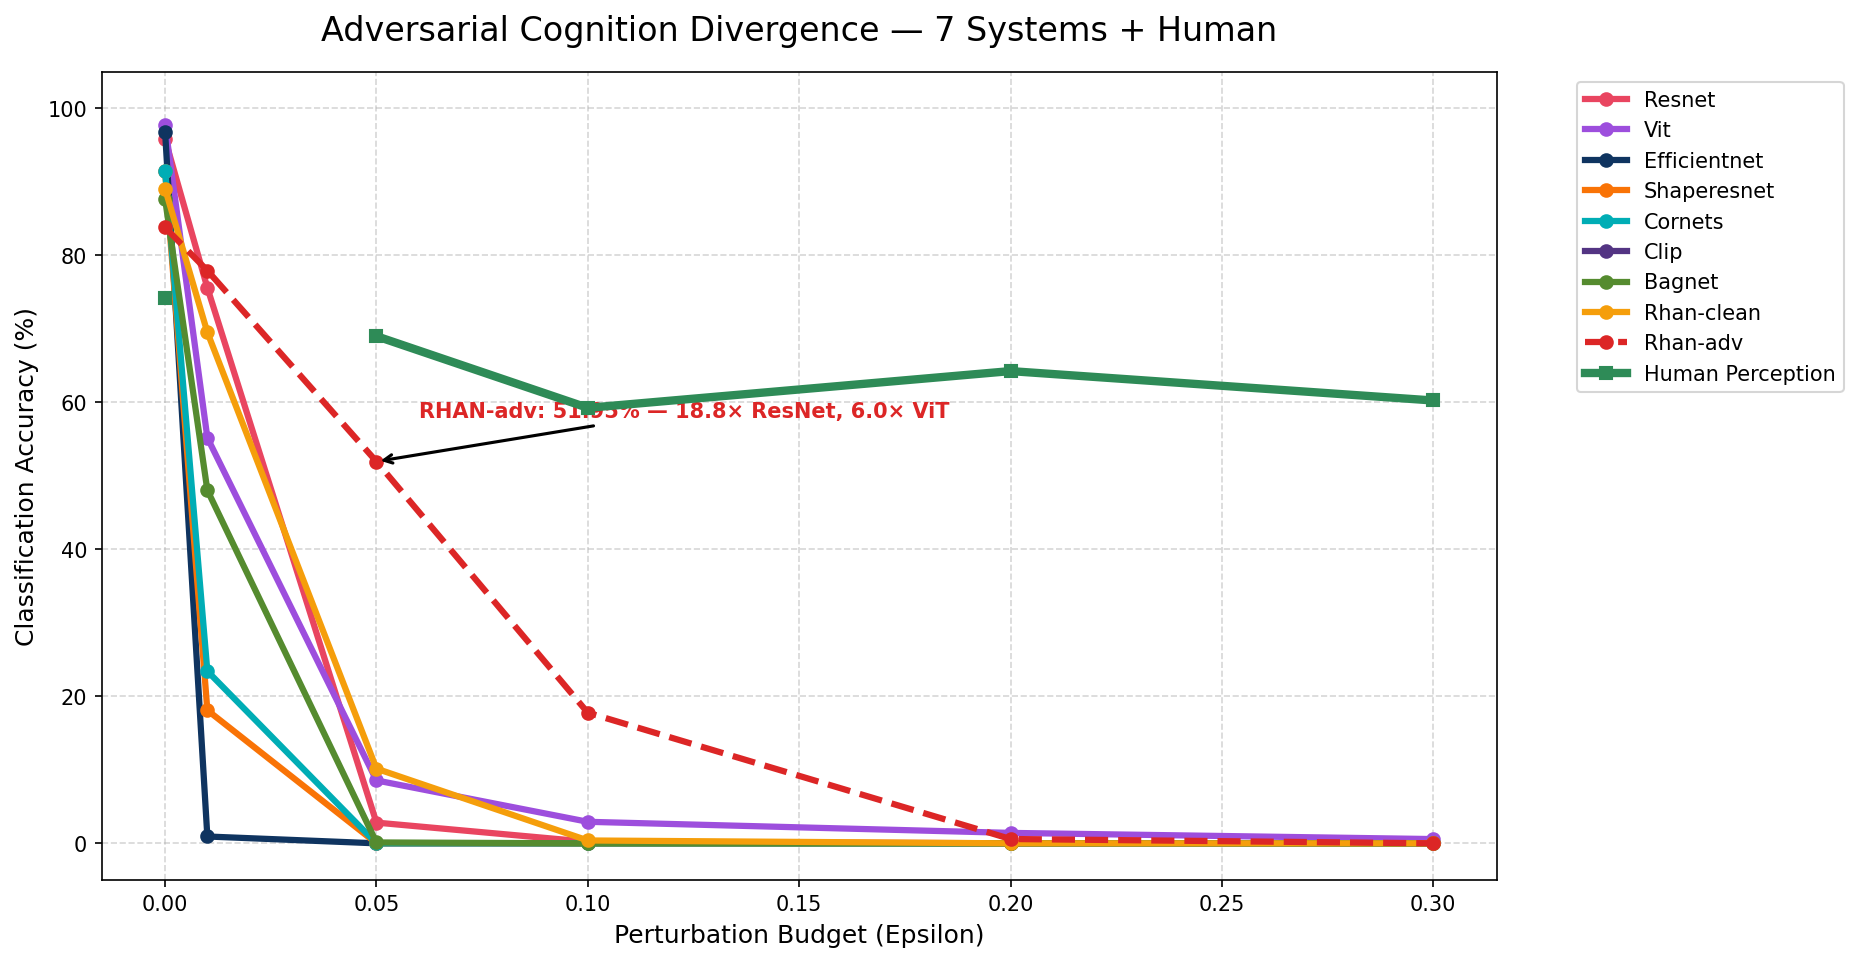
\includegraphics[width=\textwidth]{figures/FINAL_divergence_with_rhan.png}
  \caption{Accuracy divergence curves (Fig.~A.1).}
  \label{fig:div_acc_full}
\end{subfigure}
\hfill
\begin{subfigure}[b]{0.48\textwidth}
  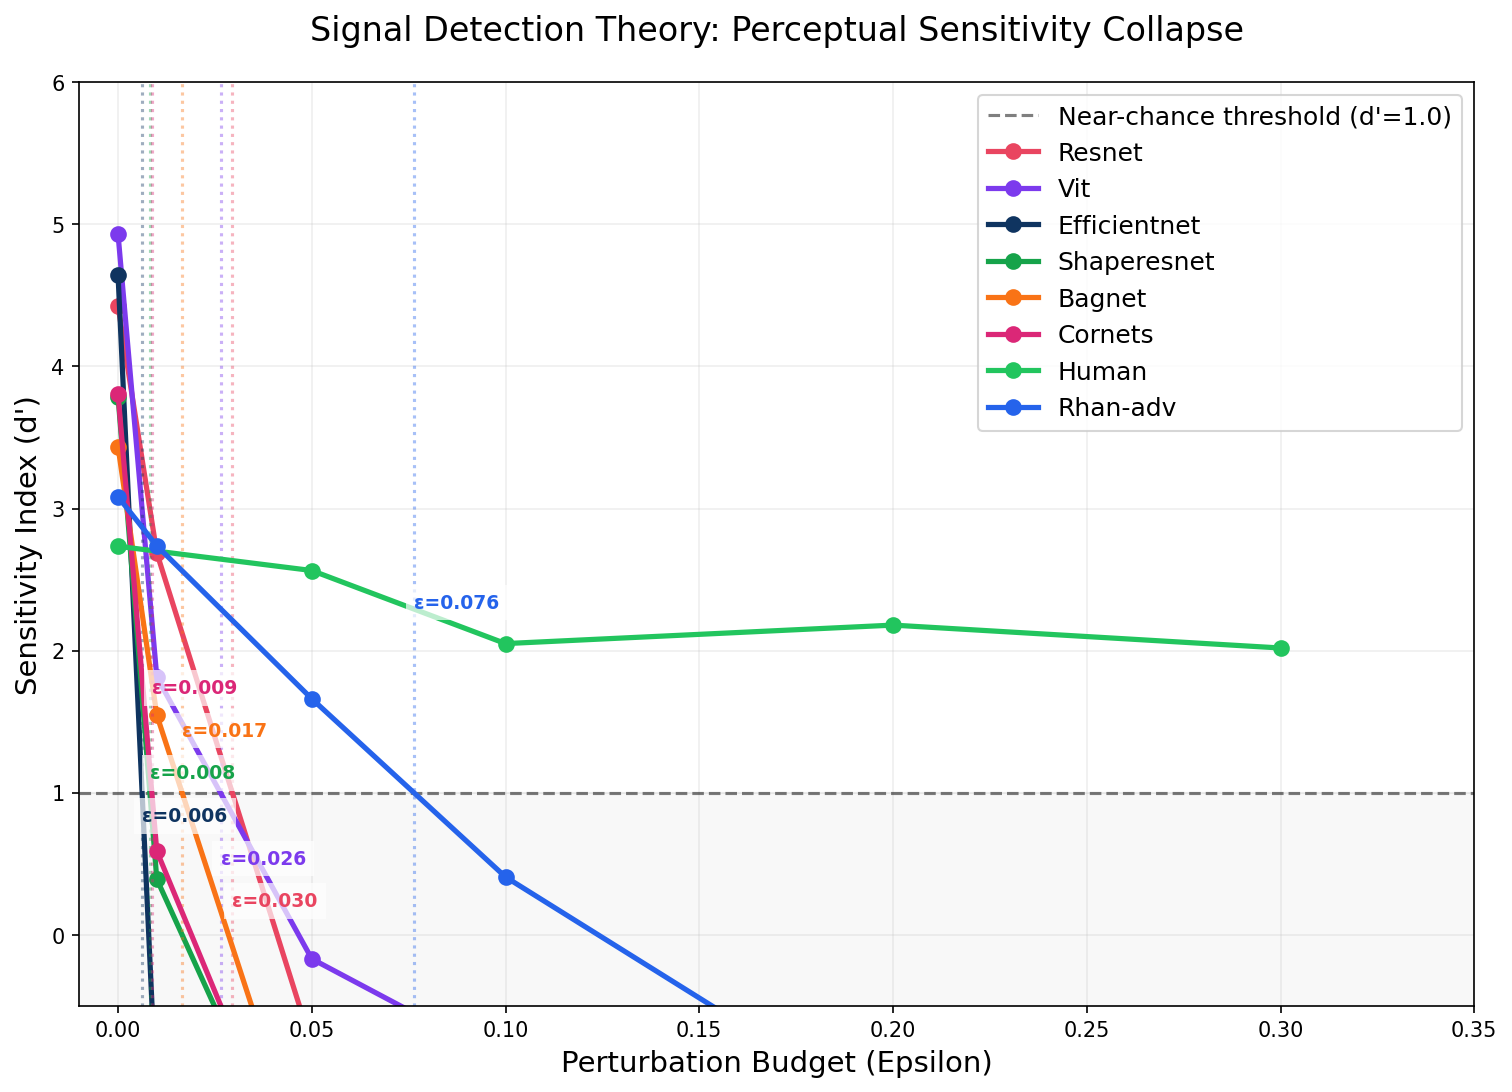
\includegraphics[width=\textwidth]{figures/final_dprime_with_rhan.png}
  \caption{SDT $d'$ sensitivity curves (Fig.~A.2).}
  \label{fig:div_dprime_full}
\end{subfigure}
\caption{\textbf{Unified Accuracy and Perceptual Sensitivity Curves}
across seven architectures and human vision. Panel (a) illustrates the
absolute accuracy decay across epsilon budgets. Panel (b) normalizes
sensitivity via $d'$, showing that RHAN-adv is the only machine system
to maintain $d' > 1.0$ beyond $\varepsilon = 0.05$.}
\label{fig:unified_curves_full}
\end{figure}

\begin{figure}[H]
\centering
\begin{subfigure}[b]{0.48\textwidth}
  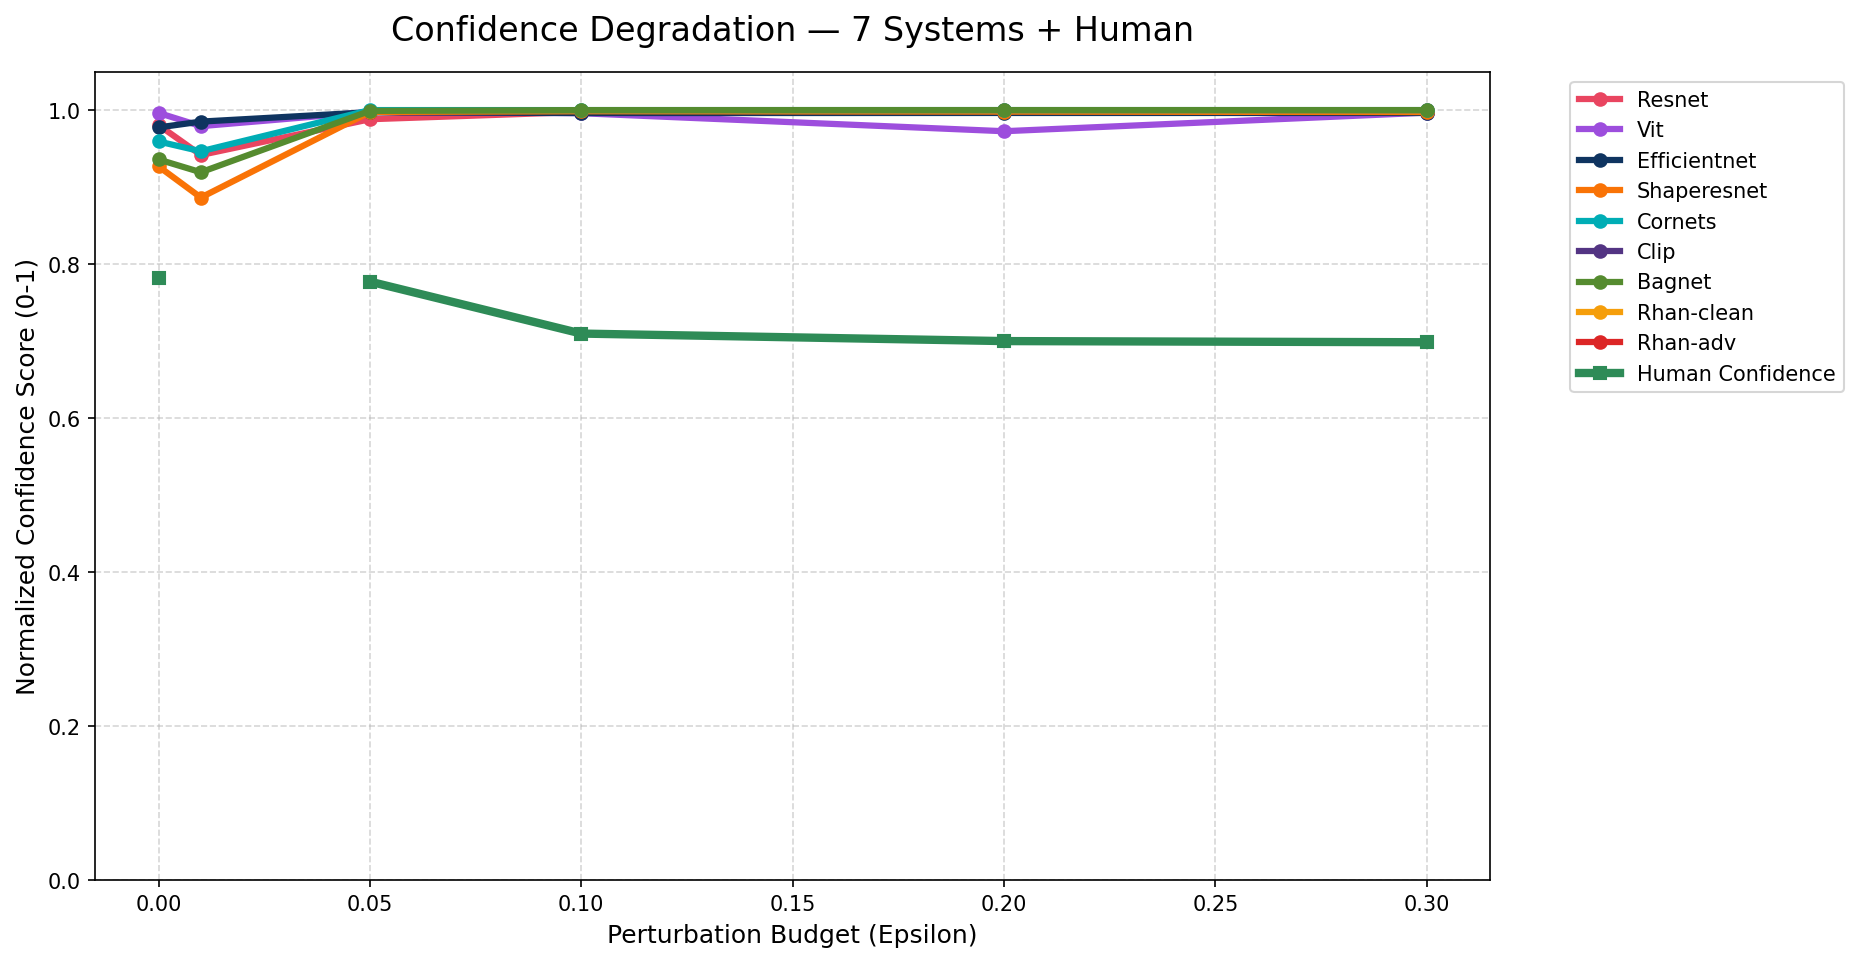
\includegraphics[width=\textwidth]{figures/full_confidence_curve.png}
  \caption{Confidence decay curves (Fig.~A.3).}
  \label{fig:confidence_decay_full}
\end{subfigure}
\hfill
\begin{subfigure}[b]{0.48\textwidth}
  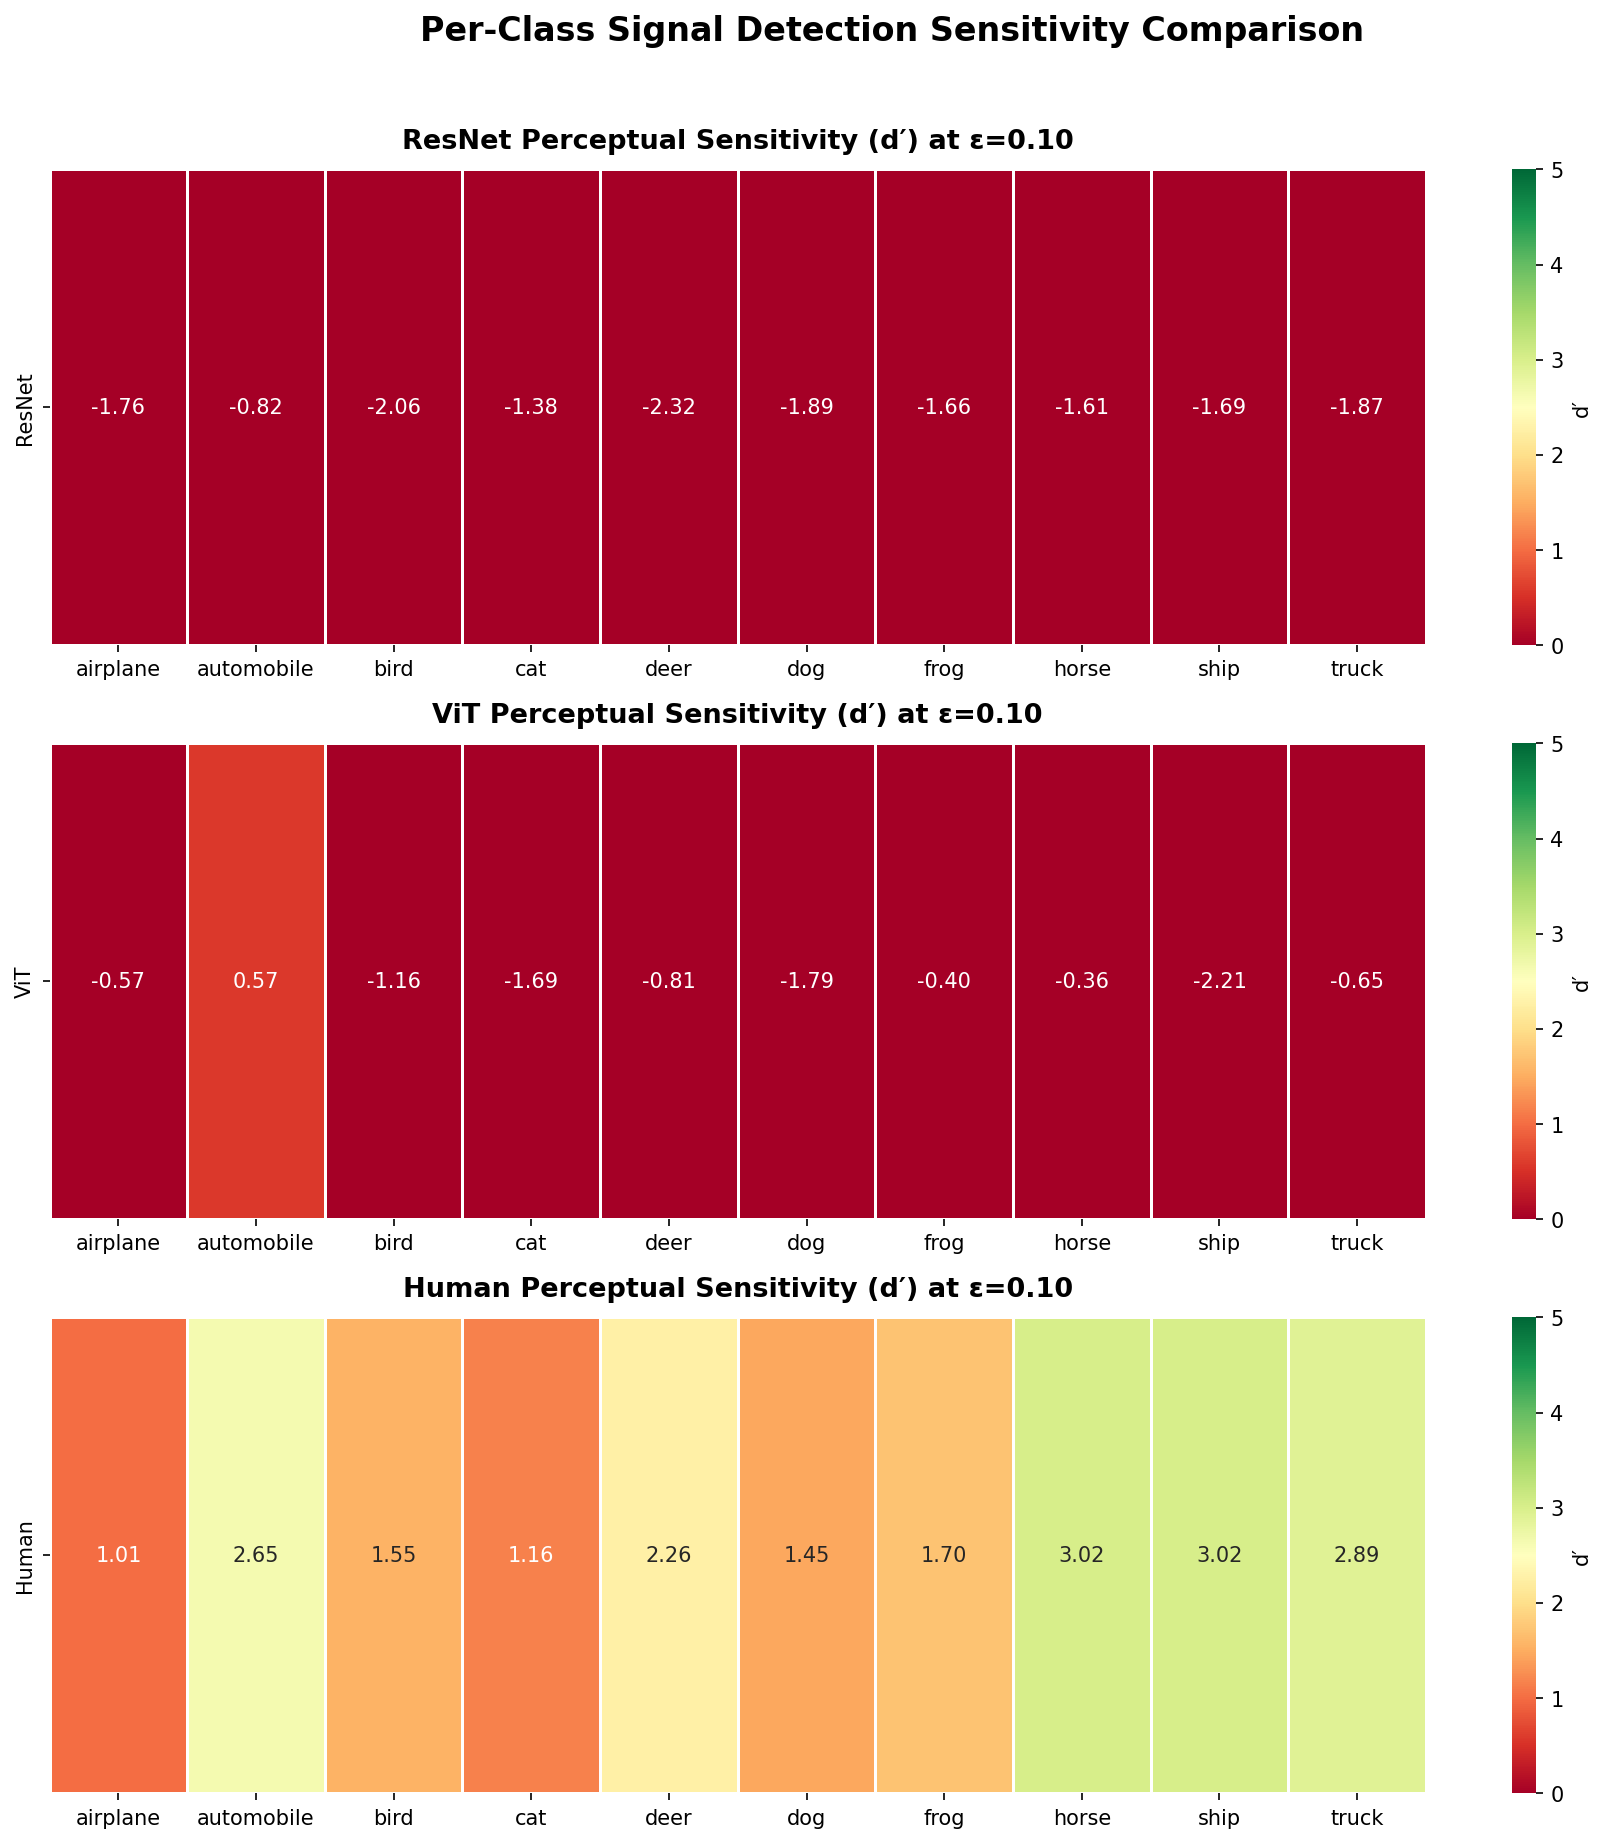
\includegraphics[width=\textwidth]{figures/perclass_dprime_eps0.10.png}
  \caption{Per-class $d'$ at $\varepsilon{=}0.10$ (Fig.~A.4).}
  \label{fig:perclass_dprime_full}
\end{subfigure}
\caption{\textbf{Confidence Calibration and Semantic Class Sensitivity}.
Panel (a) shows the normalized confidence degradation across epsilon
budgets. Panel (b) displays the per-class d-prime values at
$\varepsilon = 0.10$ demonstrating varying visual robust levels across
the CIFAR-10 classes.}
\label{fig:confidence_and_perclass_full}
\end{figure}

\begin{figure}[H]
\centering
\begin{subfigure}[b]{0.48\textwidth}
  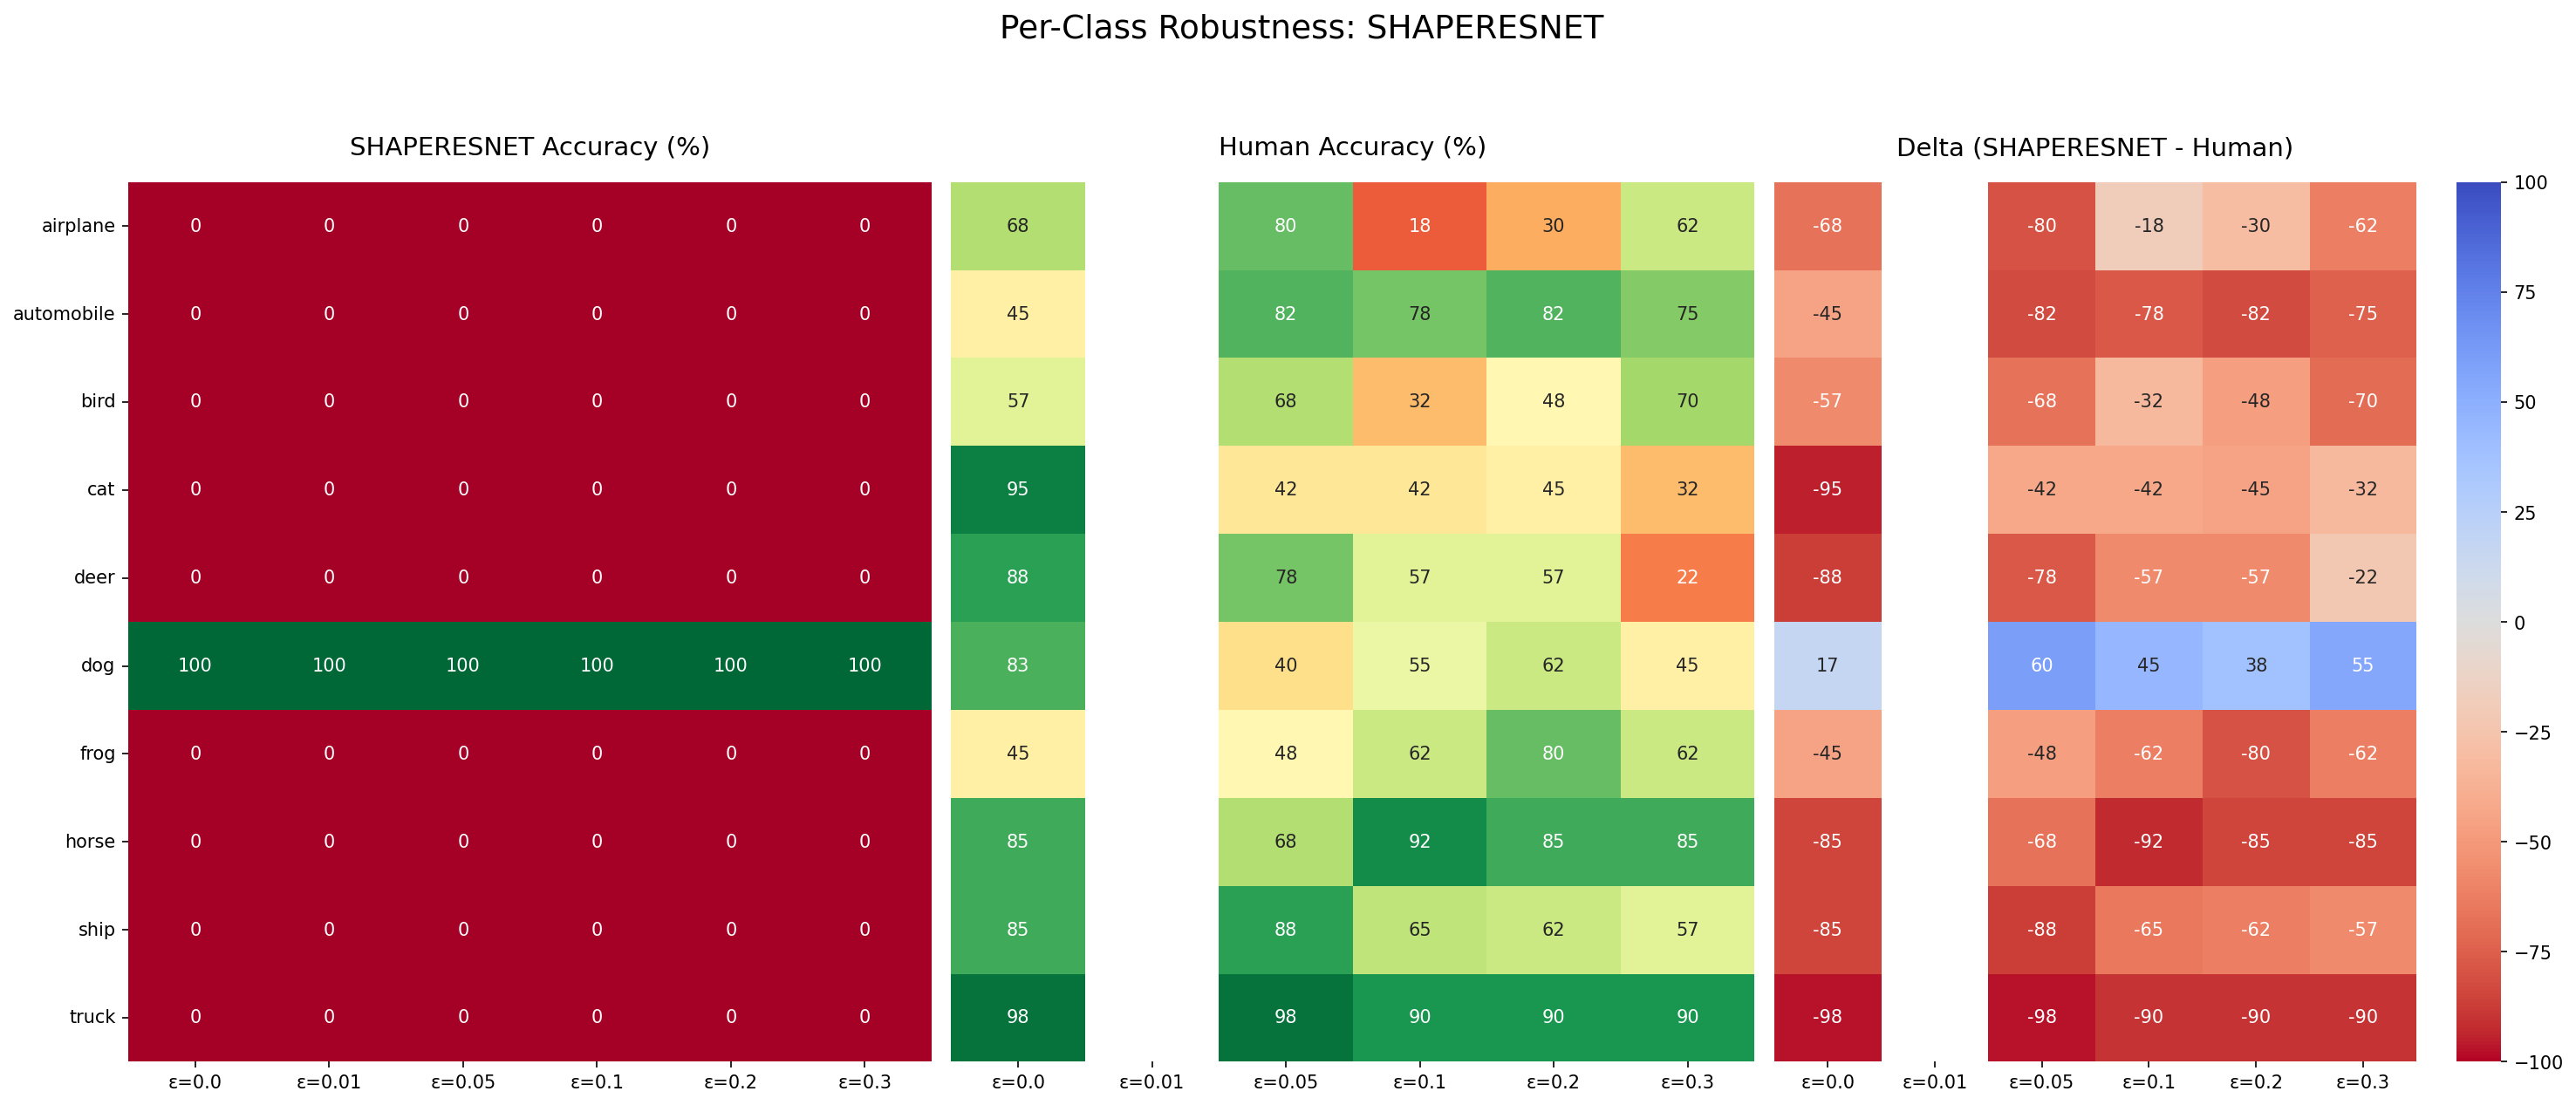
\includegraphics[width=\textwidth]{figures/class_heatmap.png}
  \caption{Machine Performance Accuracy Heatmap (Fig.~A.5).}
  \label{fig:machine_heatmap}
\end{subfigure}
\hfill
\begin{subfigure}[b]{0.48\textwidth}
  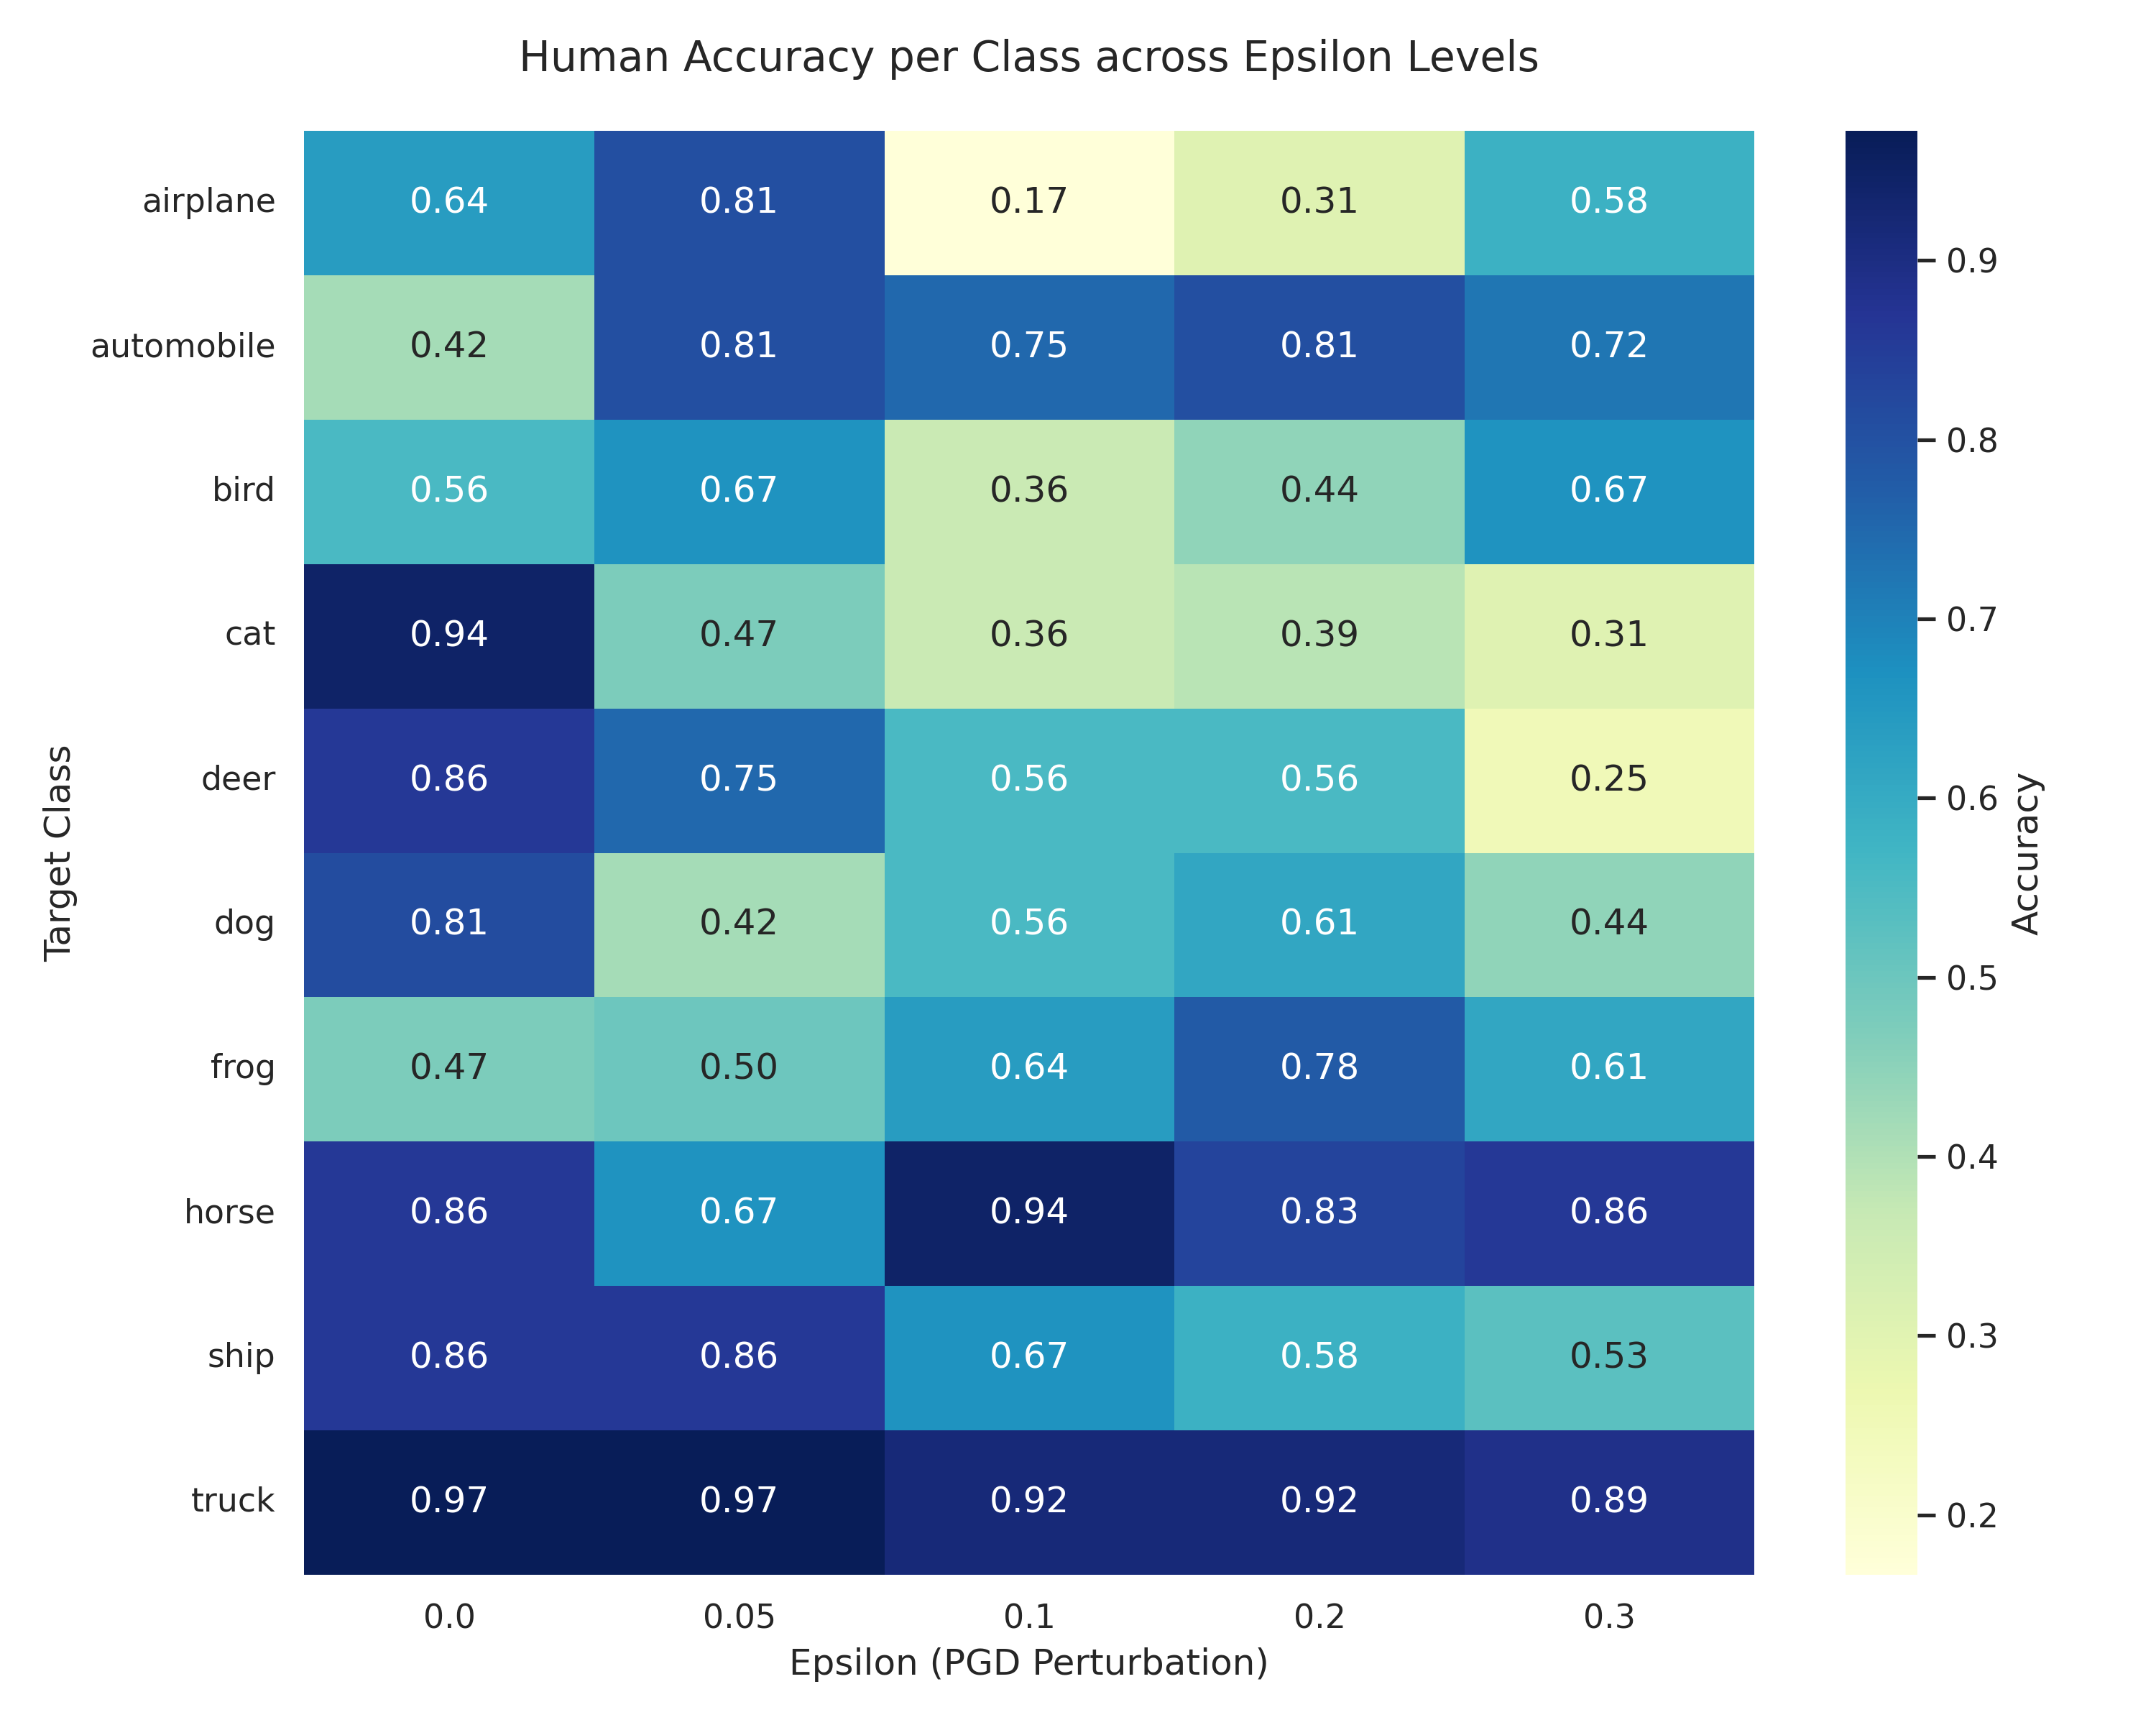
\includegraphics[width=\textwidth]{figures/human_class_heatmap.png}
  \caption{Human Performance Accuracy Heatmap (Fig.~A.6).}
  \label{fig:human_heatmap}
\end{subfigure}
\caption{\textbf{Semantic Class Accuracy Heatmaps across Epsilon Budgets}.
Panel (a) and Panel (b) provide a side-by-side comparative
visualization of classification accuracy per class as perturbation
budgets scale.}
\label{fig:class_heatmaps}
\end{figure}

\begin{figure}[H]
\centering
\begin{subfigure}[b]{0.48\textwidth}
  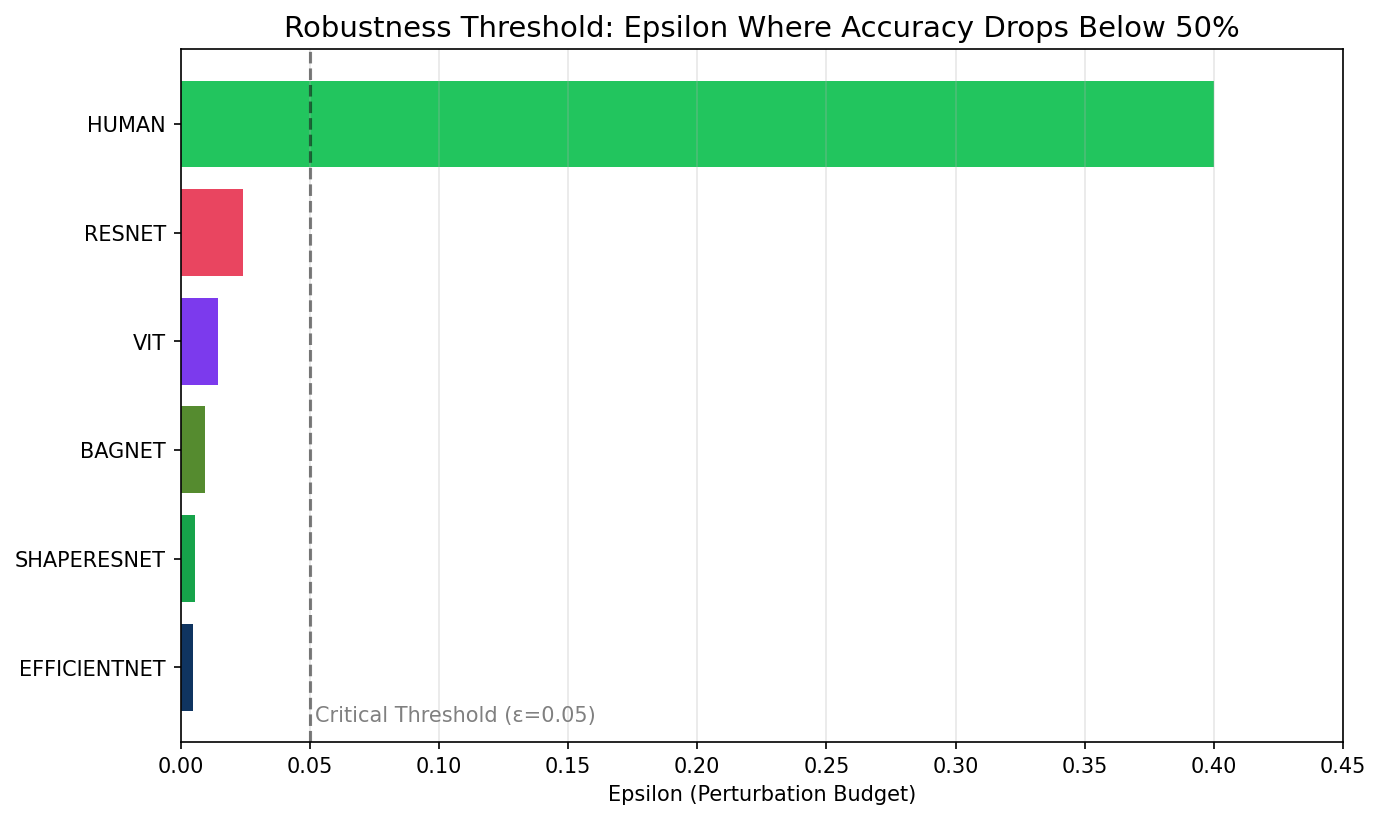
\includegraphics[width=\textwidth]{figures/accuracy_threshold_bars.png}
  \caption{Accuracy-based Thresholds (Fig.~A.7).}
  \label{fig:acc_thresholds}
\end{subfigure}
\hfill
\begin{subfigure}[b]{0.48\textwidth}
  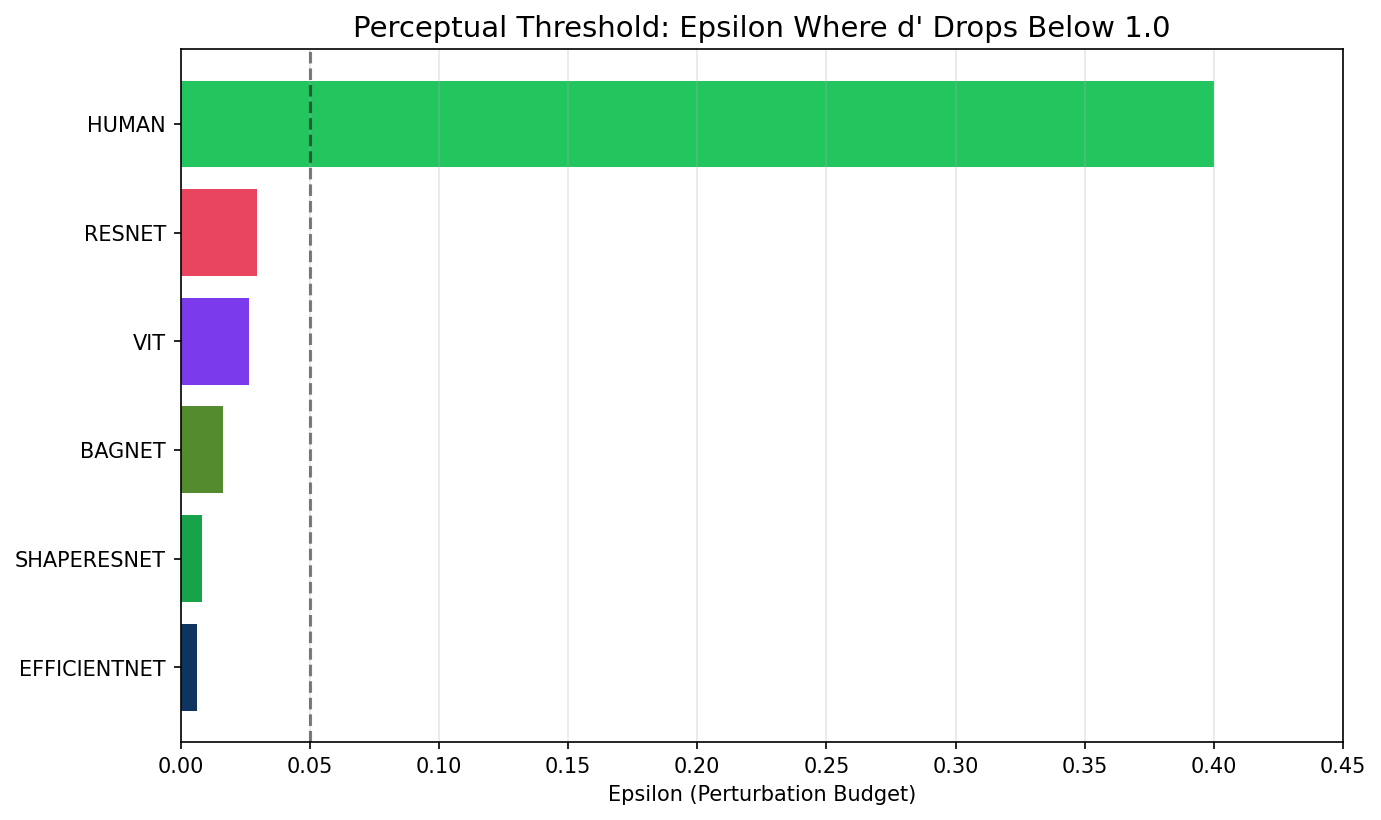
\includegraphics[width=\textwidth]{figures/sdt_threshold_bars.png}
  \caption{SDT Sensitivity Thresholds (Fig.~A.8).}
  \label{fig:sdt_thresholds}
\end{subfigure}
\caption{\textbf{Empirical and Perceptual Robustness Thresholds}.
Panel (a) shows raw accuracy thresholds. Panel (b) displays the SDT
sensitivity thresholds ($\varepsilon_{\text{thresh}}$ where $d' < 1.0$).}
\label{fig:threshold_bars}
\end{figure}

\subsection{Representation and Latent Space Topology}

\begin{figure}[H]
\centering
\begin{subfigure}[b]{0.48\textwidth}
  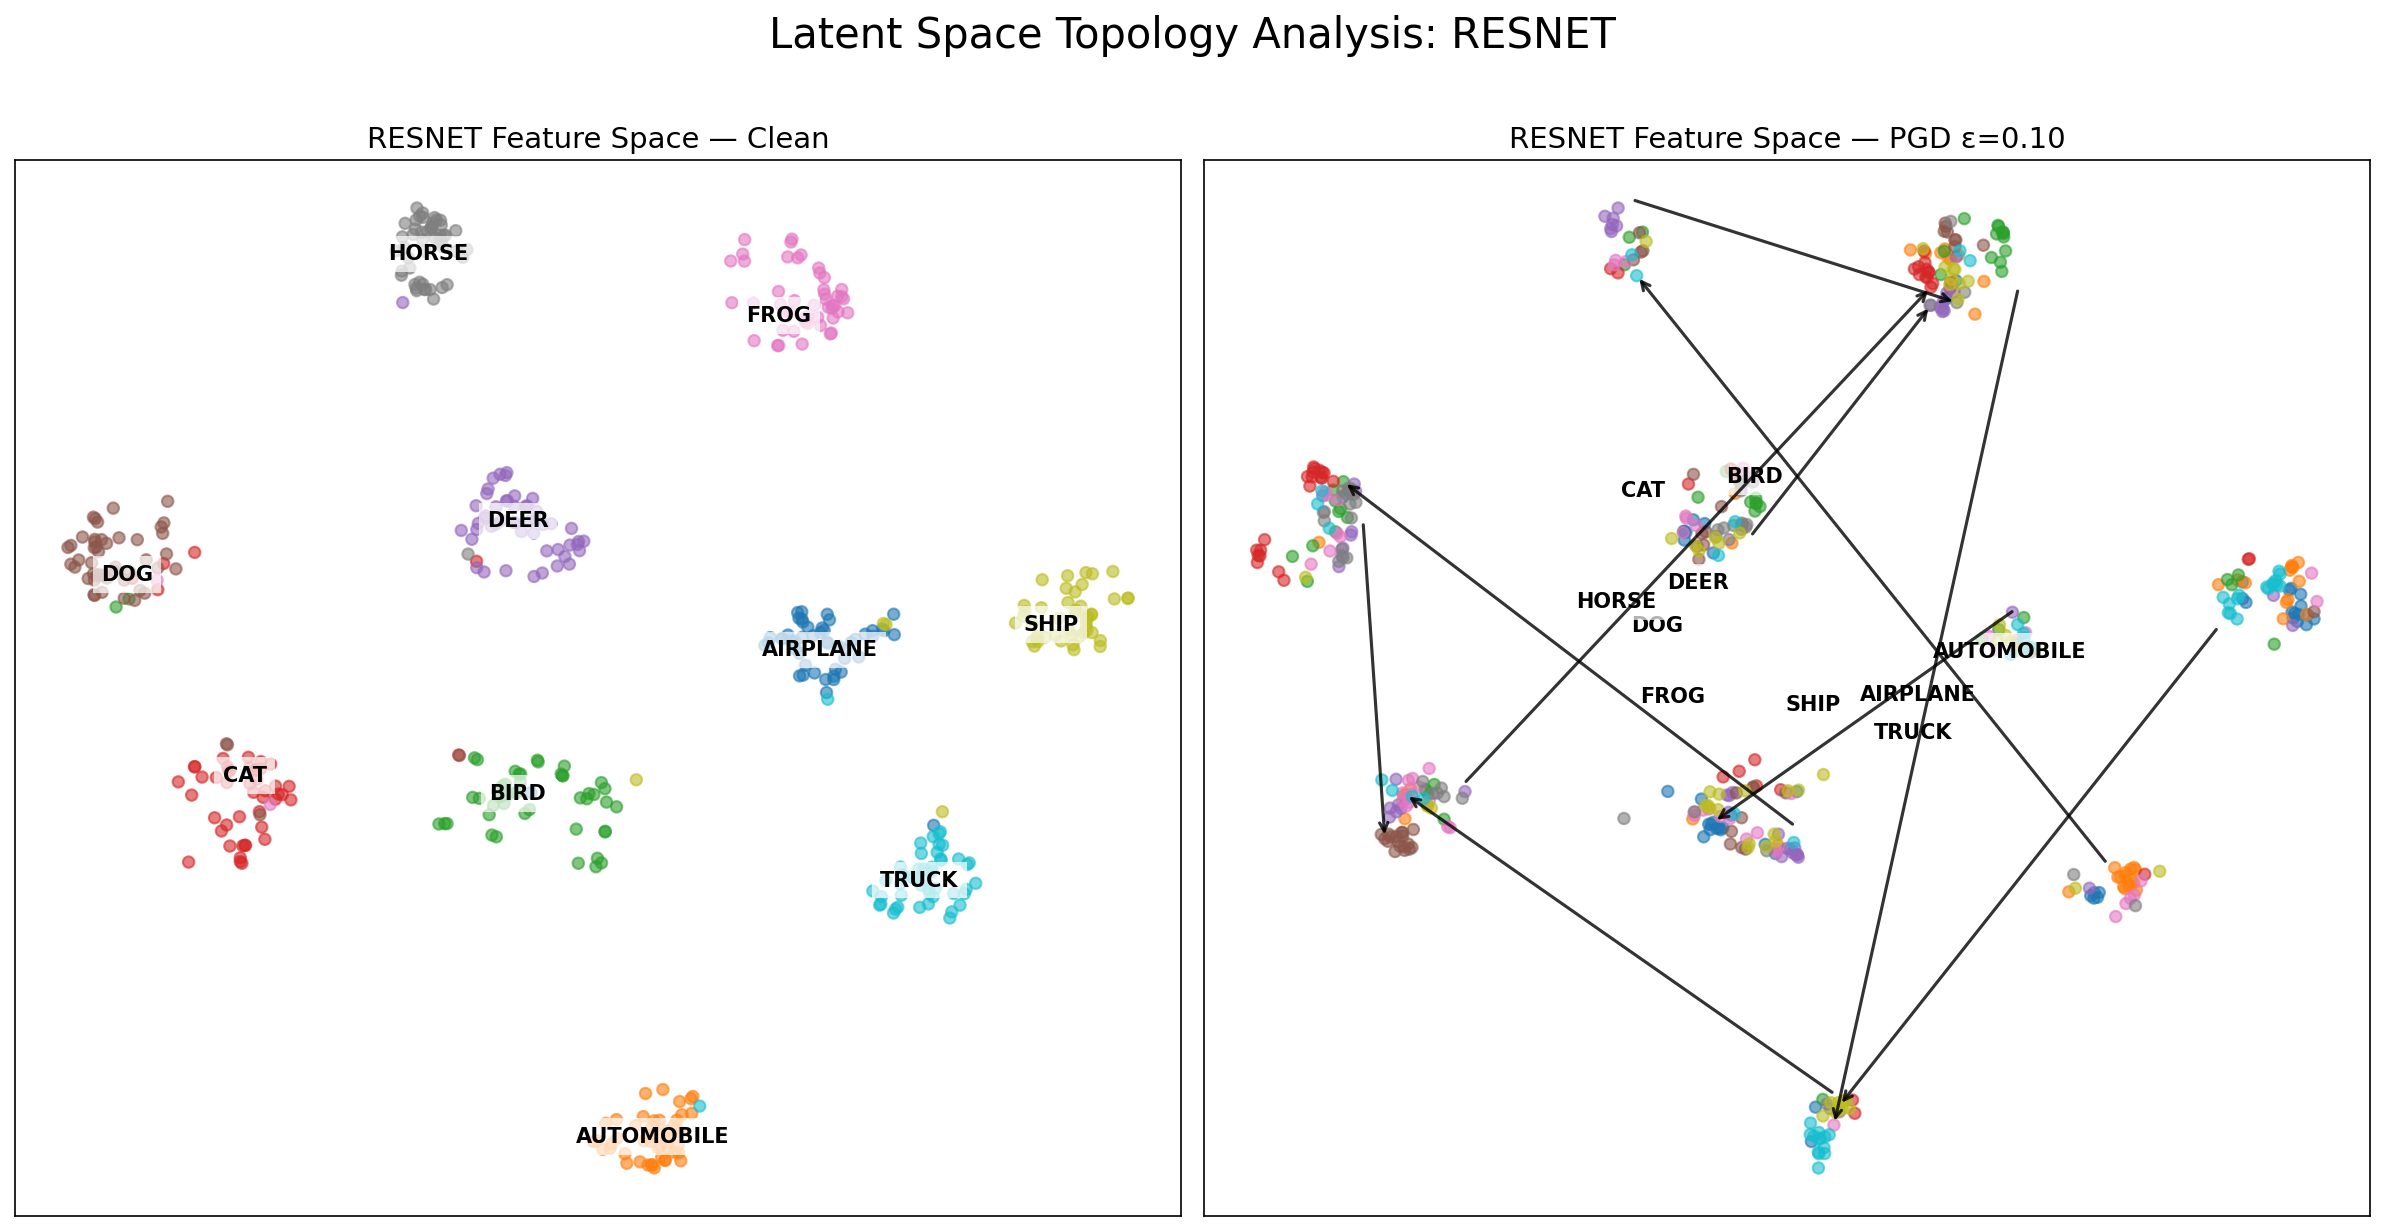
\includegraphics[width=\textwidth]{figures/resnet_tsne.png}
  \caption{ResNet-18 latent t-SNE (Fig.~A.9).}
  \label{fig:resnet_tsne_full}
\end{subfigure}
\hfill
\begin{subfigure}[b]{0.48\textwidth}
  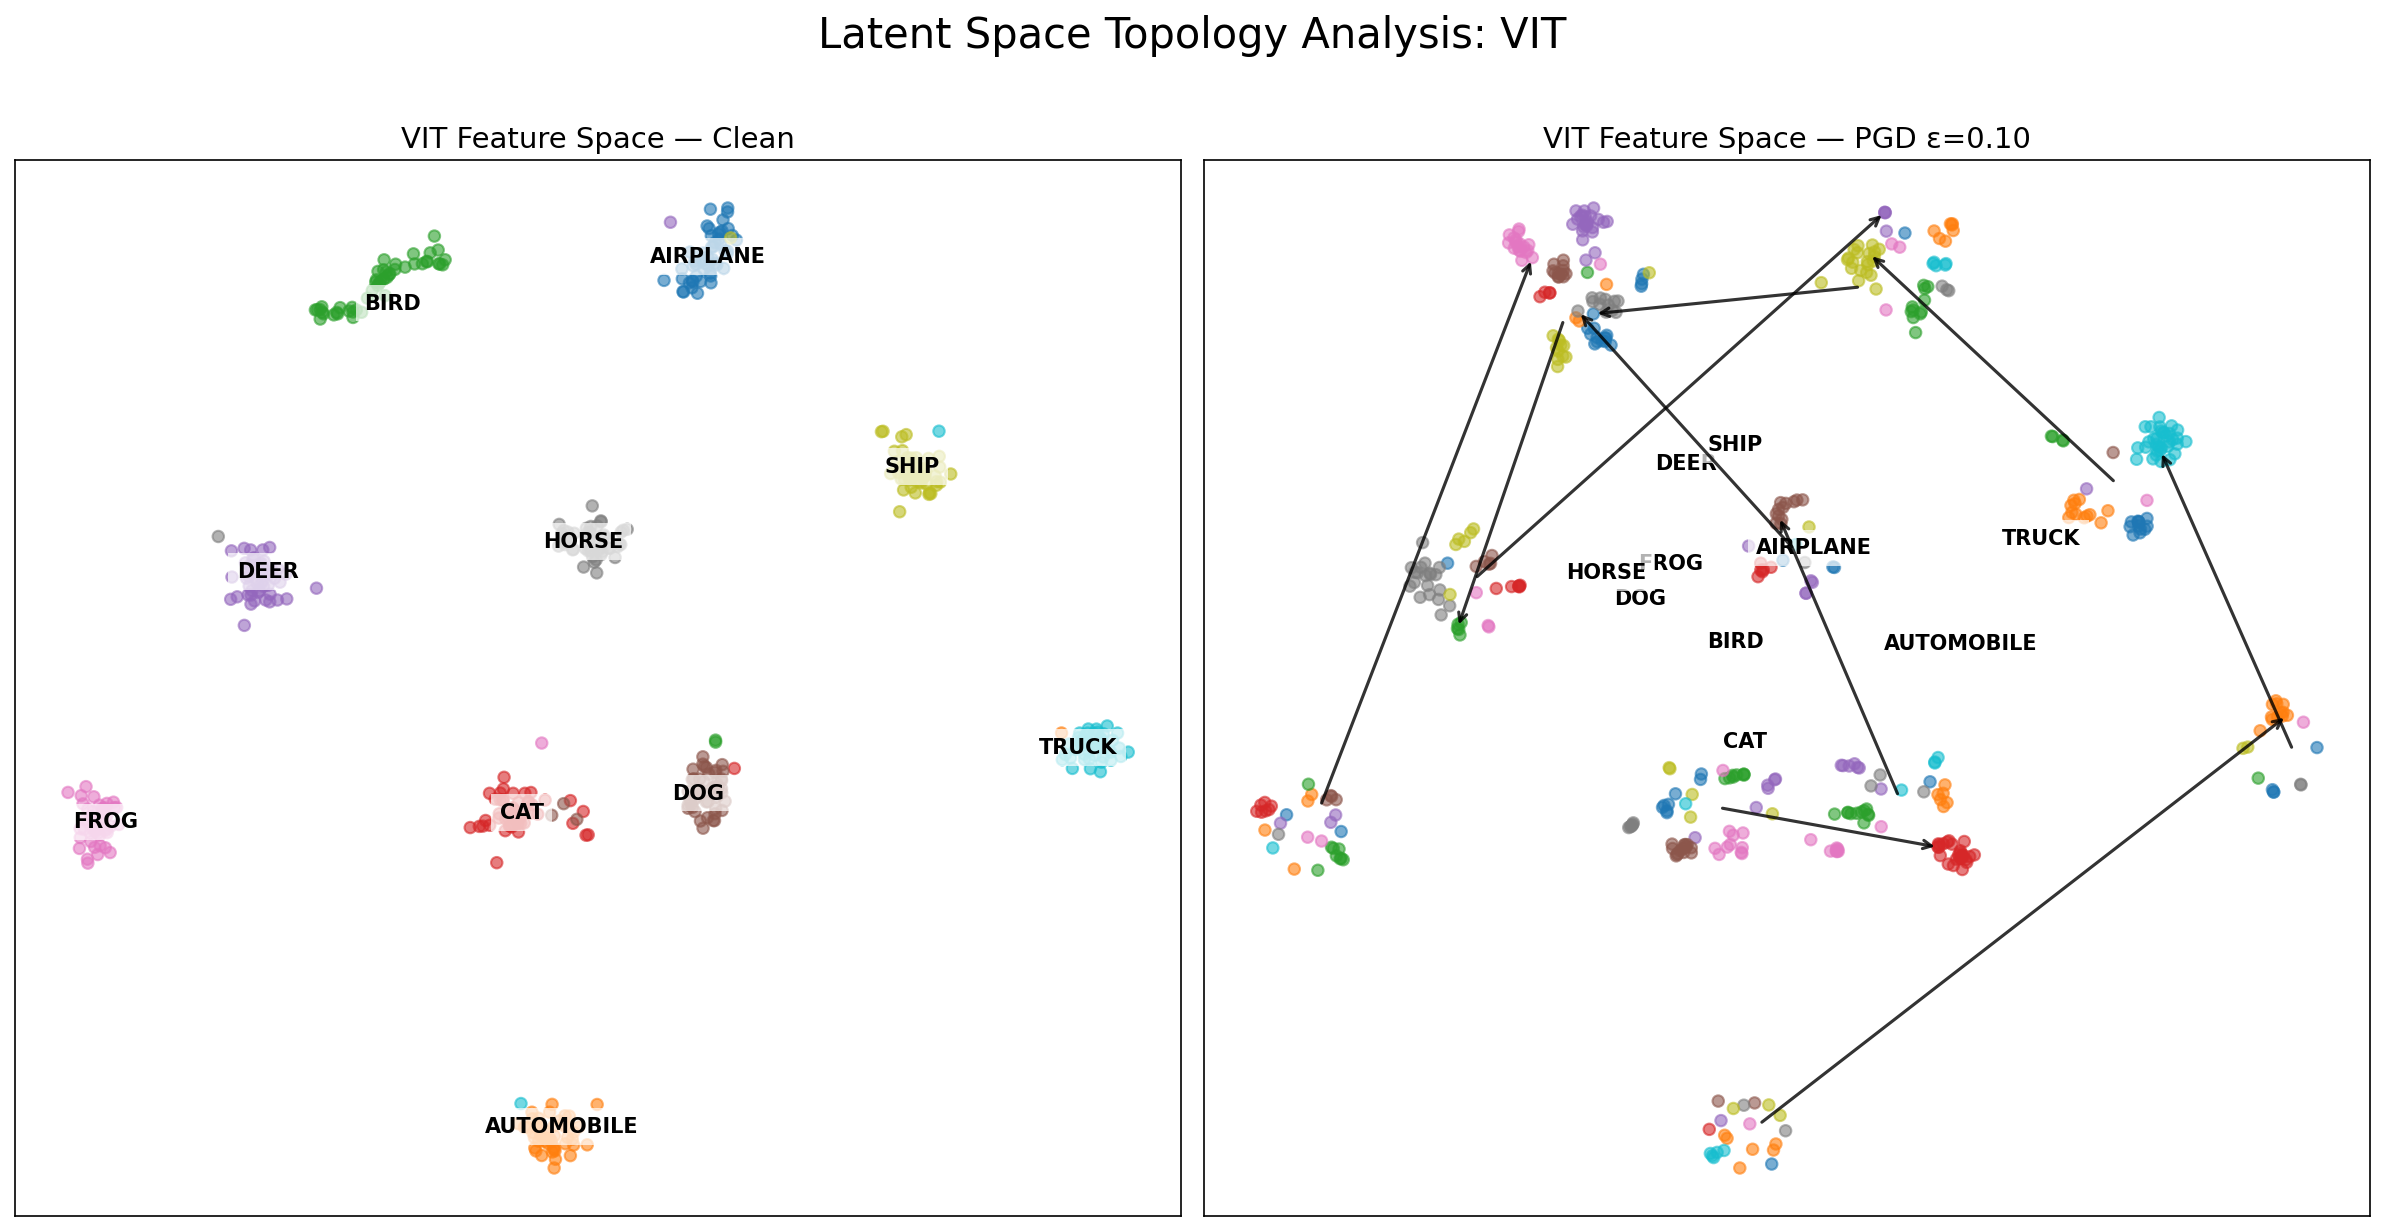
\includegraphics[width=\textwidth]{figures/vit_tsne.png}
  \caption{ViT-Small latent t-SNE (Fig.~A.10).}
  \label{fig:vit_tsne_full}
\end{subfigure}
\caption{\textbf{Latent Feature Space Displacement t-SNE Projections}.}
\label{fig:tsne_full}
\end{figure}

\begin{figure}[H]
\centering
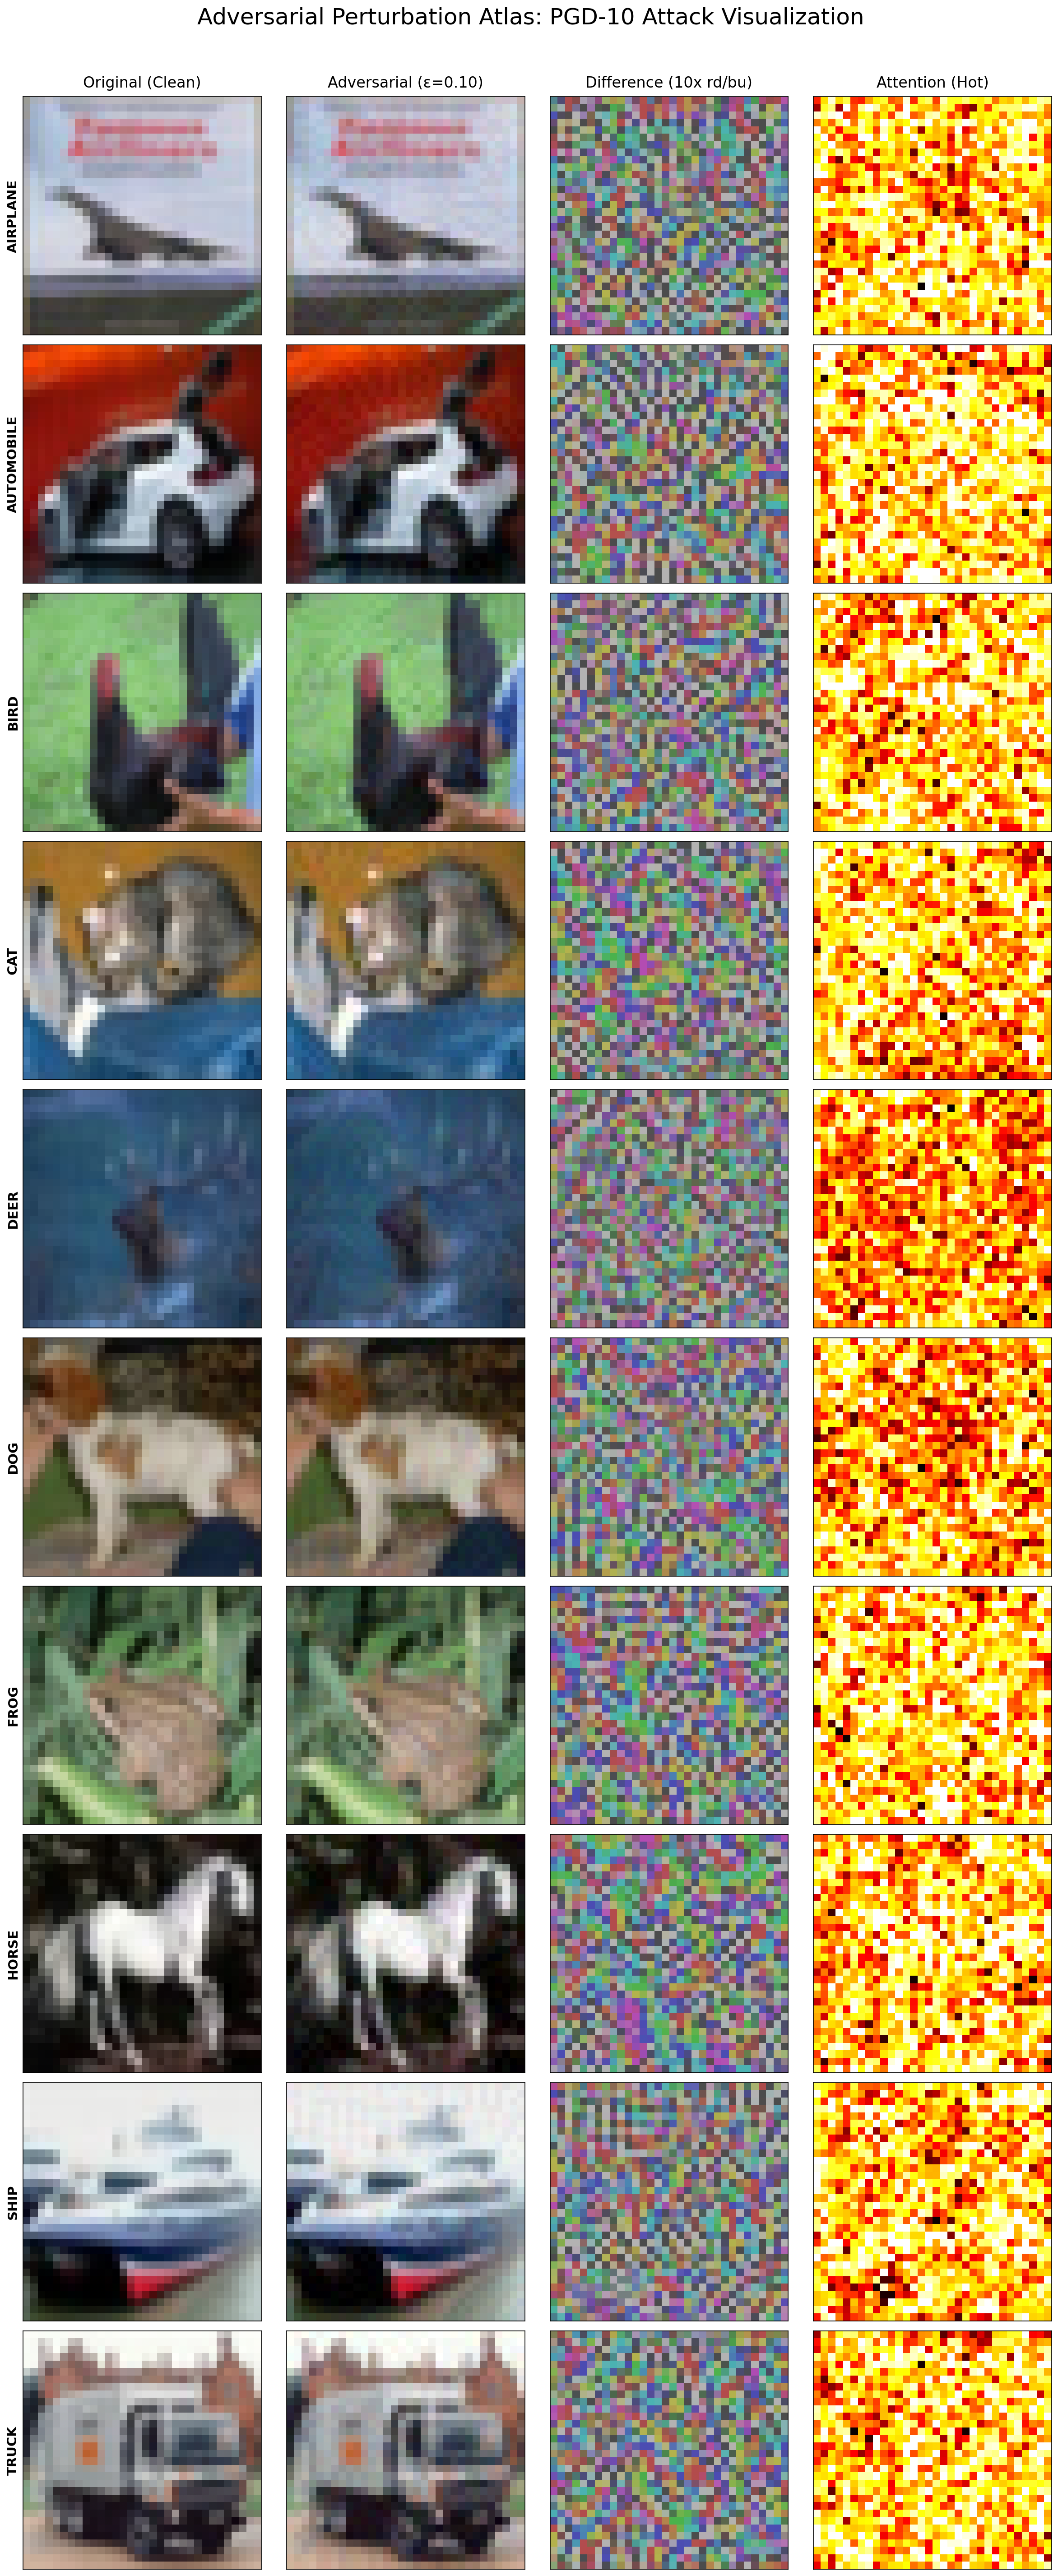
\includegraphics[width=0.9\textwidth]{figures/perturbation_atlas.png}
\caption{\textbf{The Adversarial Perturbation Atlas (Fig.~A.13)}.}
\label{fig:perturbation_atlas}
\end{figure}

\subsection{Model-Specific Confusion Matrices}

\begin{figure}[H]
\centering
\begin{subfigure}[b]{0.48\textwidth}
  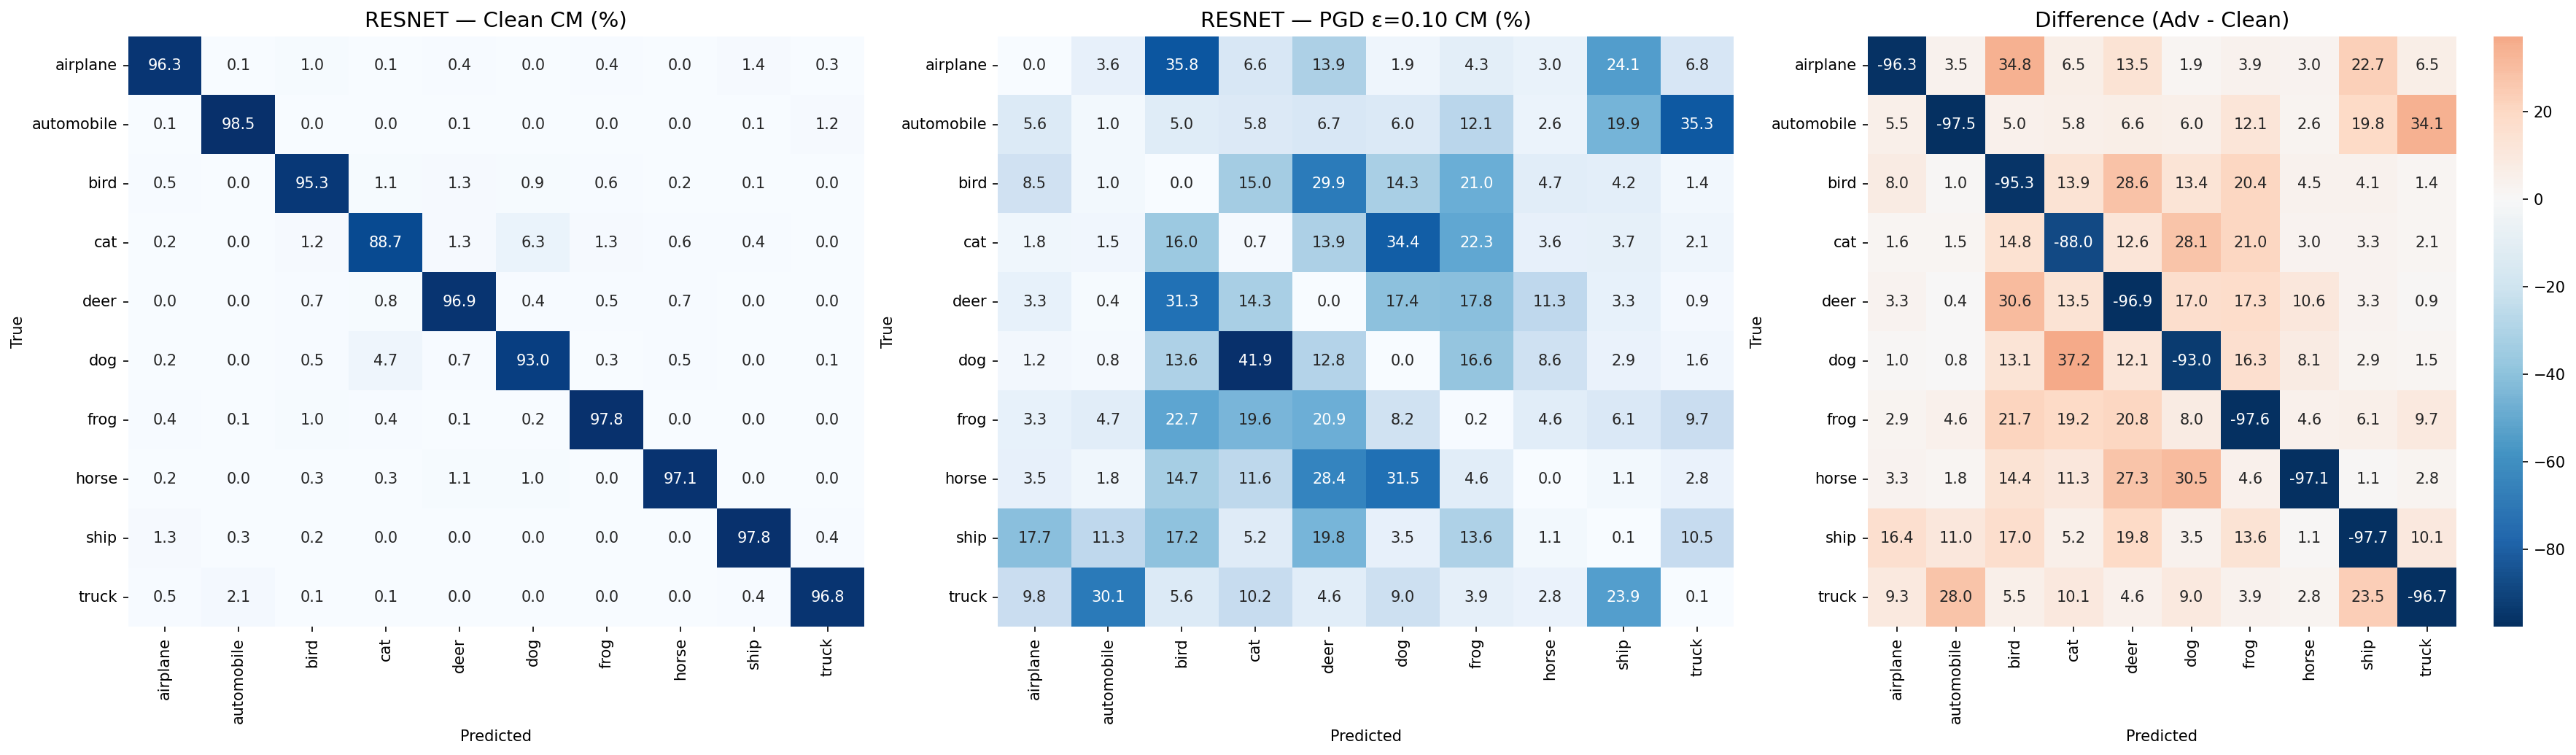
\includegraphics[width=\textwidth]{figures/resnet_confusion_suite.png}
  \caption{ResNet-18 (Fig.~A.14).}
  \label{fig:resnet_conf}
\end{subfigure}
\hfill
\begin{subfigure}[b]{0.48\textwidth}
  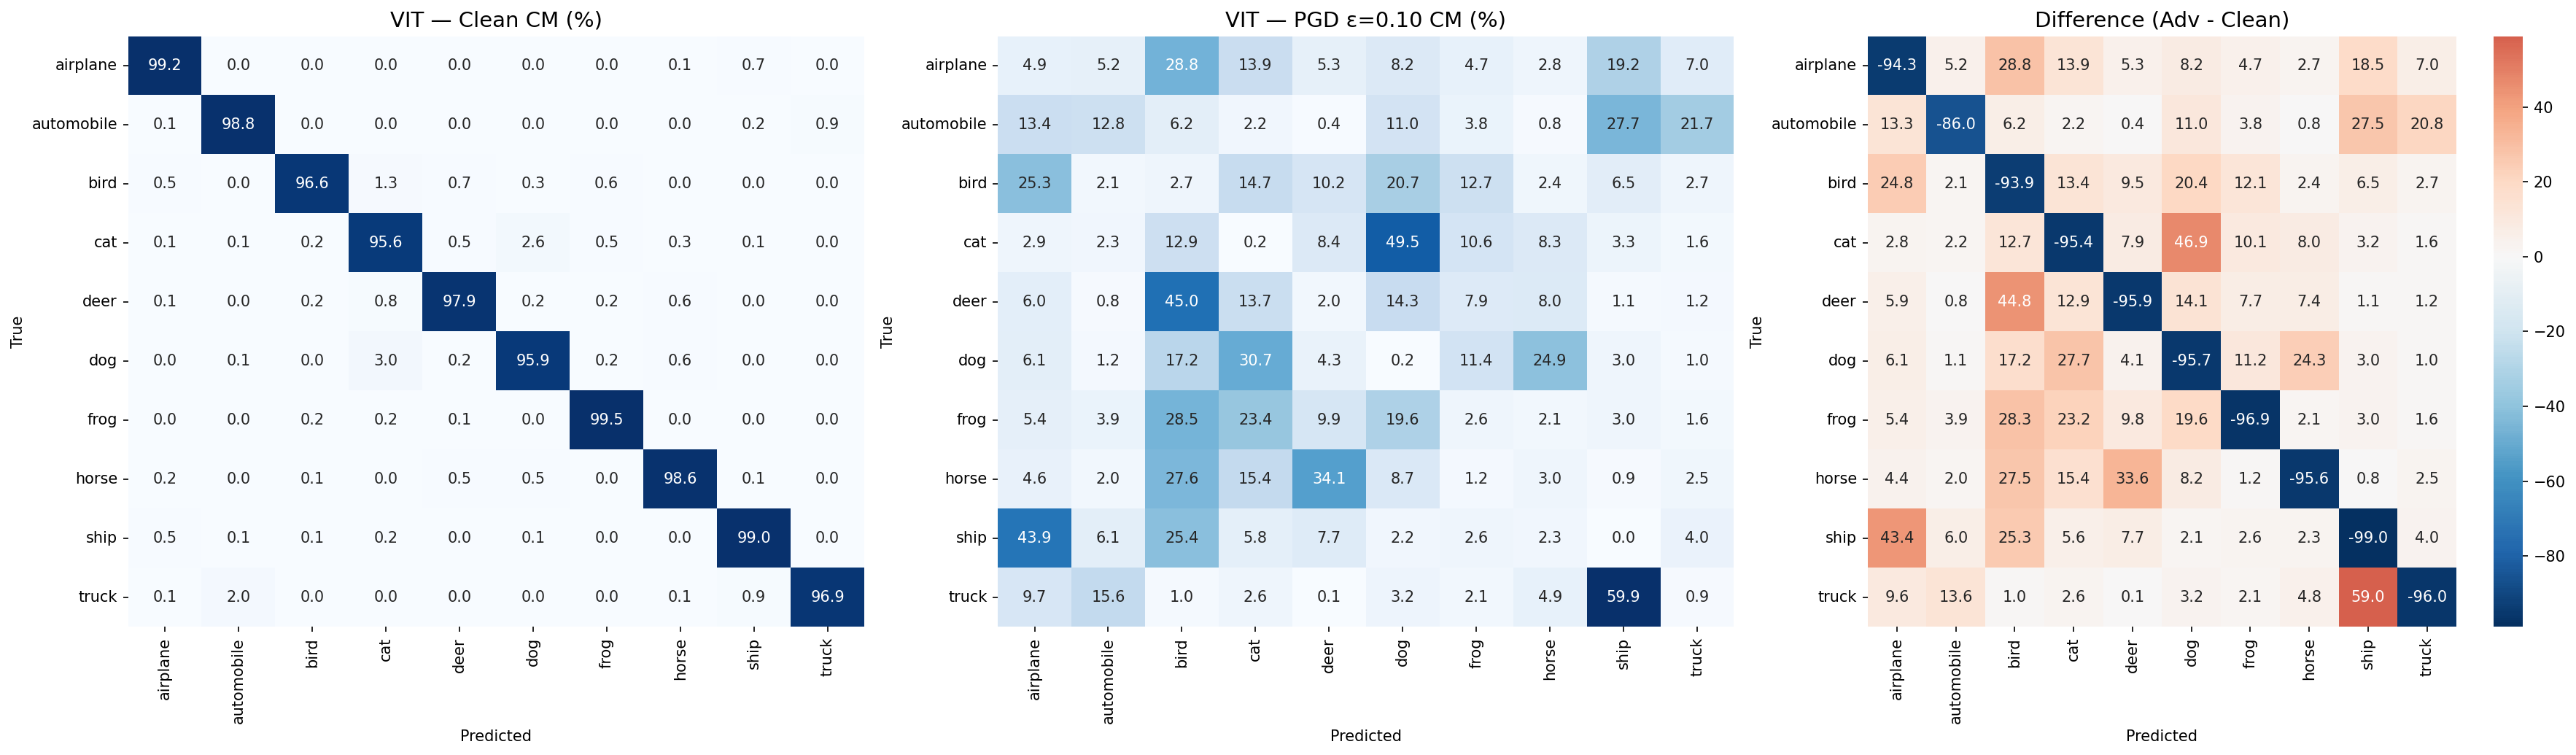
\includegraphics[width=\textwidth]{figures/vit_confusion_suite.png}
  \caption{ViT-Small (Fig.~A.15).}
  \label{fig:vit_conf}
\end{subfigure}
\caption{\textbf{Adversarial Confusion Matrices: ResNet-18 vs.\ ViT-Small}.}
\label{fig:resnet_vit_conf}
\end{figure}

\begin{figure}[H]
\centering
\begin{subfigure}[b]{0.48\textwidth}
  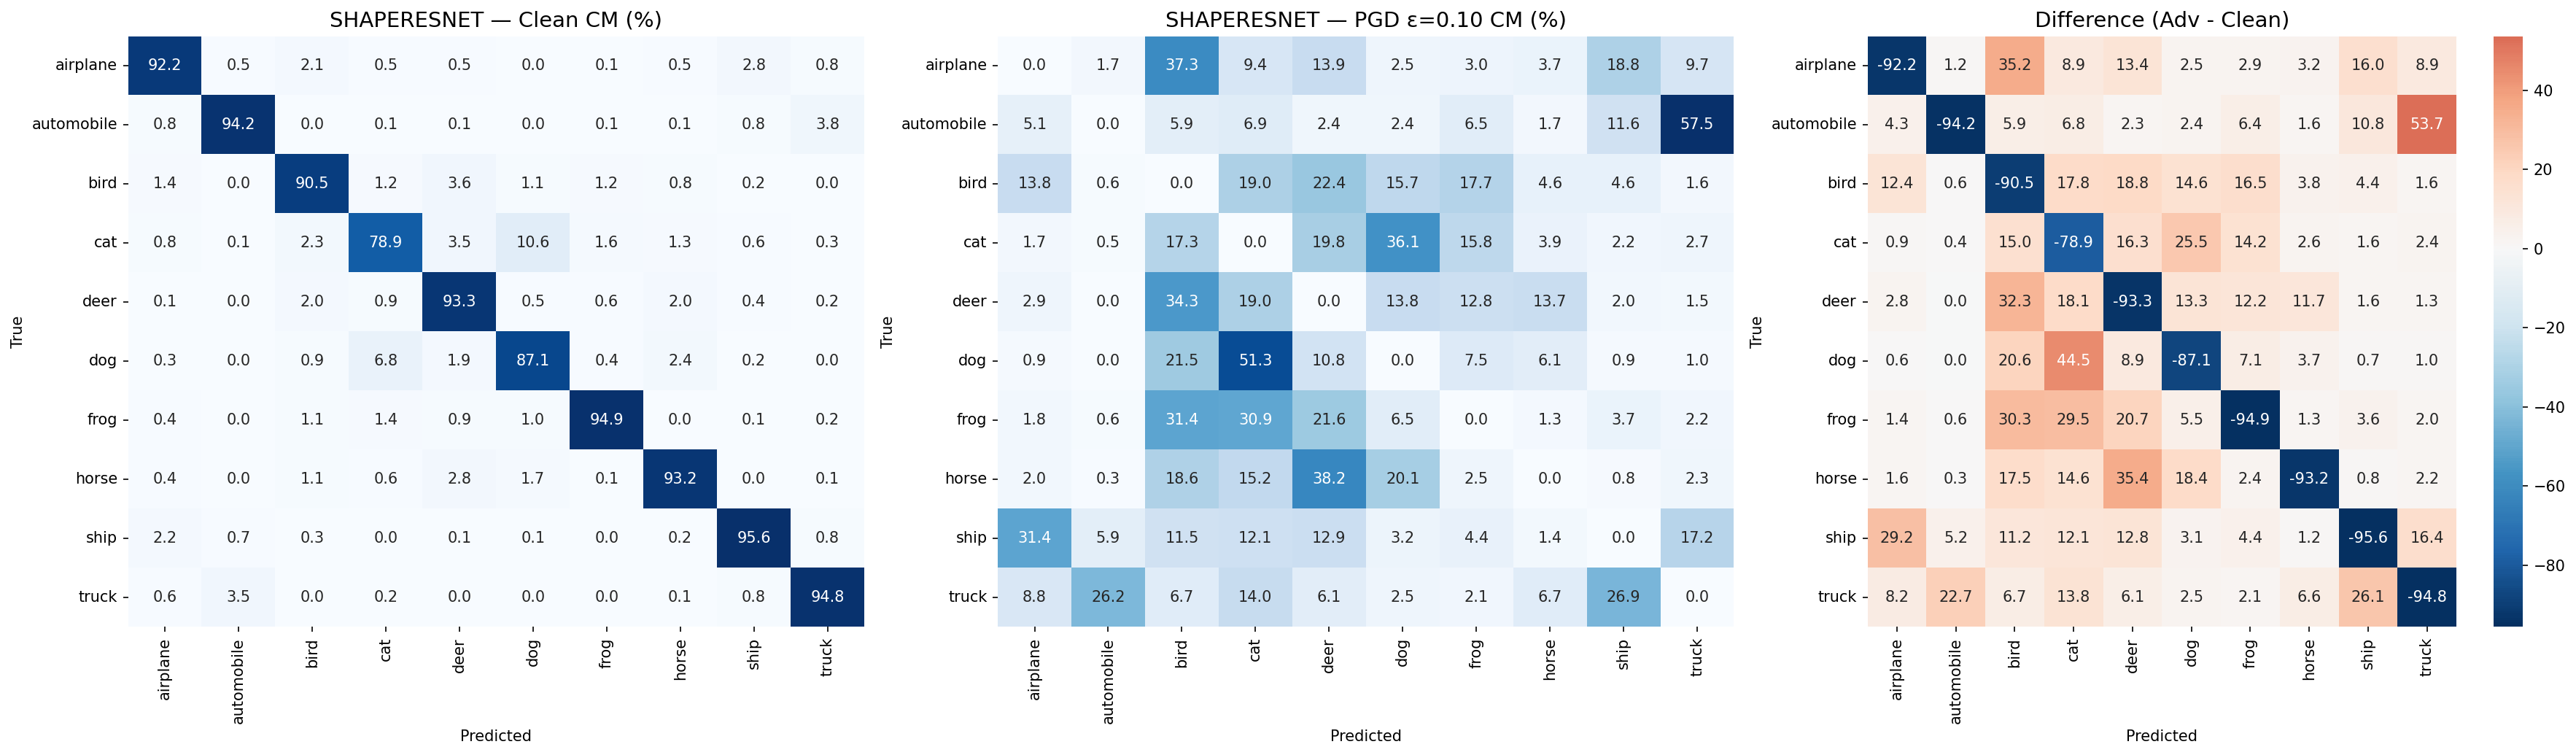
\includegraphics[width=\textwidth]{figures/shaperesnet_confusion_suite.png}
  \caption{Shape-ResNet-50 (Fig.~A.16).}
  \label{fig:shaperesnet_conf}
\end{subfigure}
\hfill
\begin{subfigure}[b]{0.48\textwidth}
  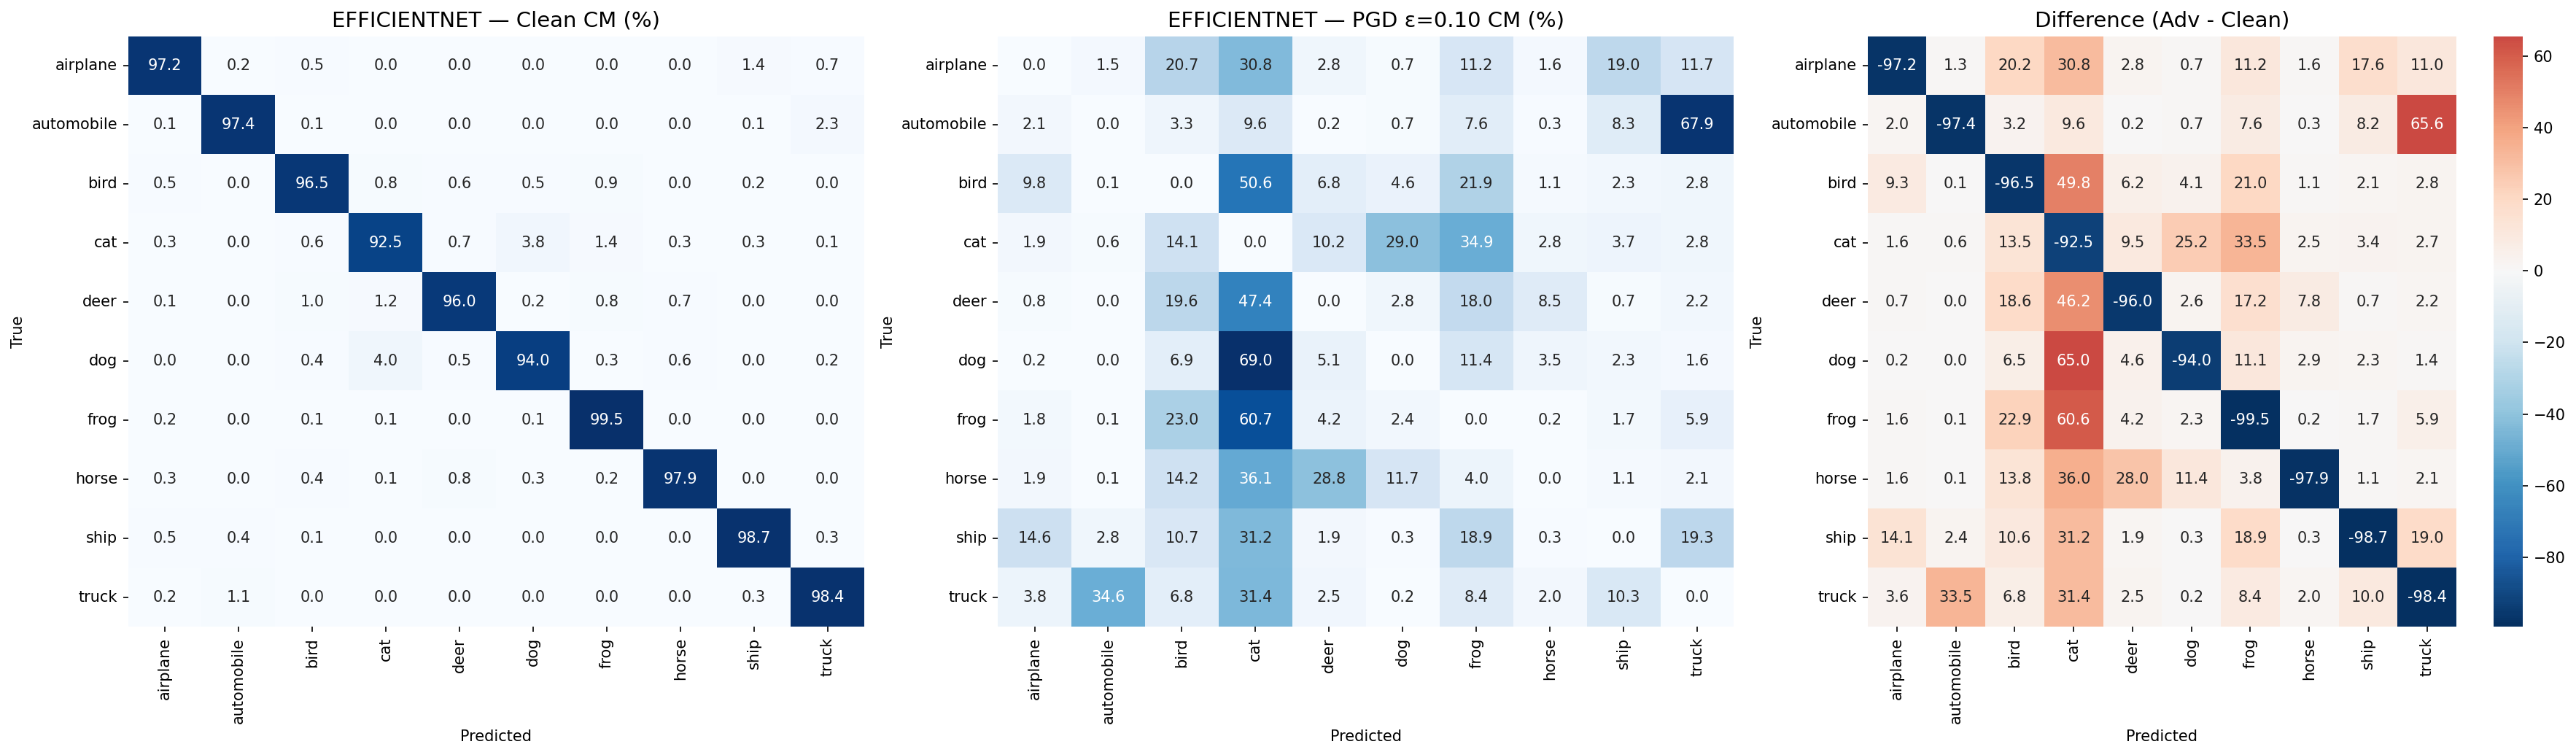
\includegraphics[width=\textwidth]{figures/efficientnet_confusion_suite.png}
  \caption{EfficientNet-B0 (Fig.~A.17).}
  \label{fig:efficientnet_conf}
\end{subfigure}
\caption{\textbf{Alternative Feedforward Confusion Suites}.}
\label{fig:alternative_conf}
\end{figure}

\begin{figure}[H]
\centering
\begin{subfigure}[b]{0.48\textwidth}
  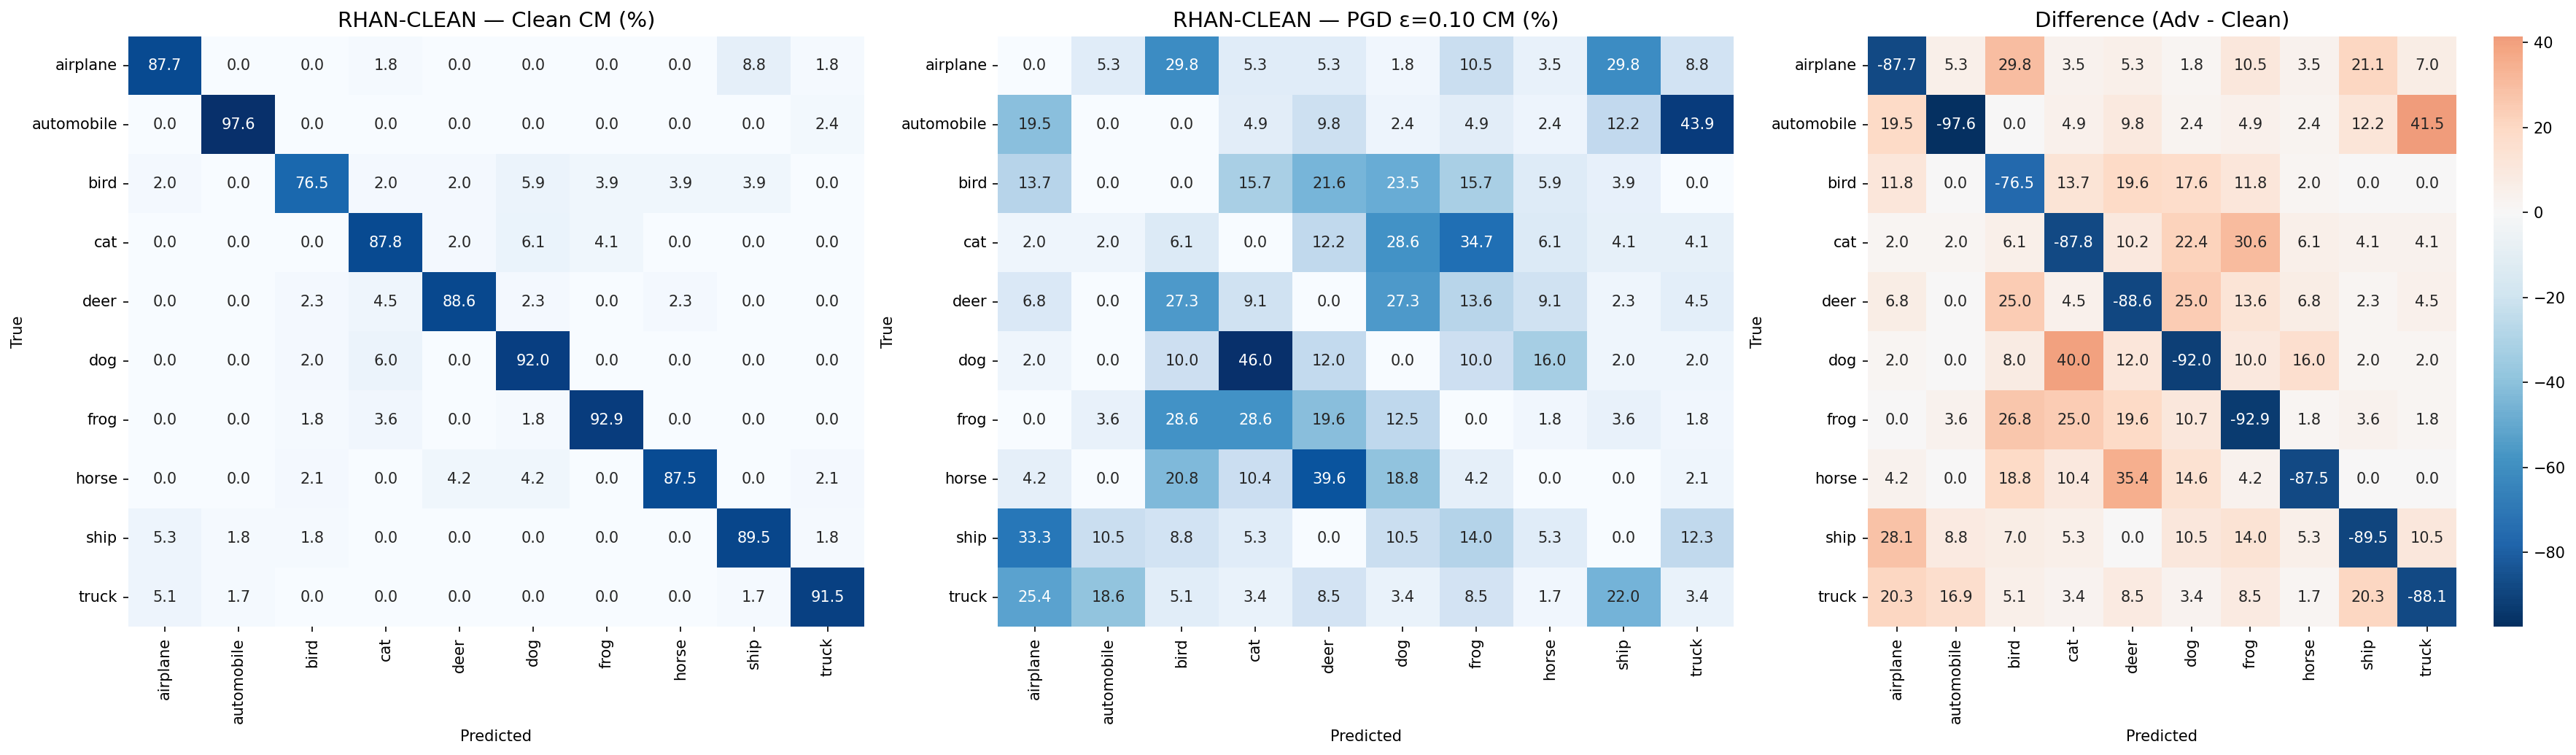
\includegraphics[width=\textwidth]{figures/rhan-clean_confusion_suite.png}
  \caption{RHAN-clean (Fig.~A.18).}
  \label{fig:rhan_clean_conf}
\end{subfigure}
\hfill
\begin{subfigure}[b]{0.48\textwidth}
  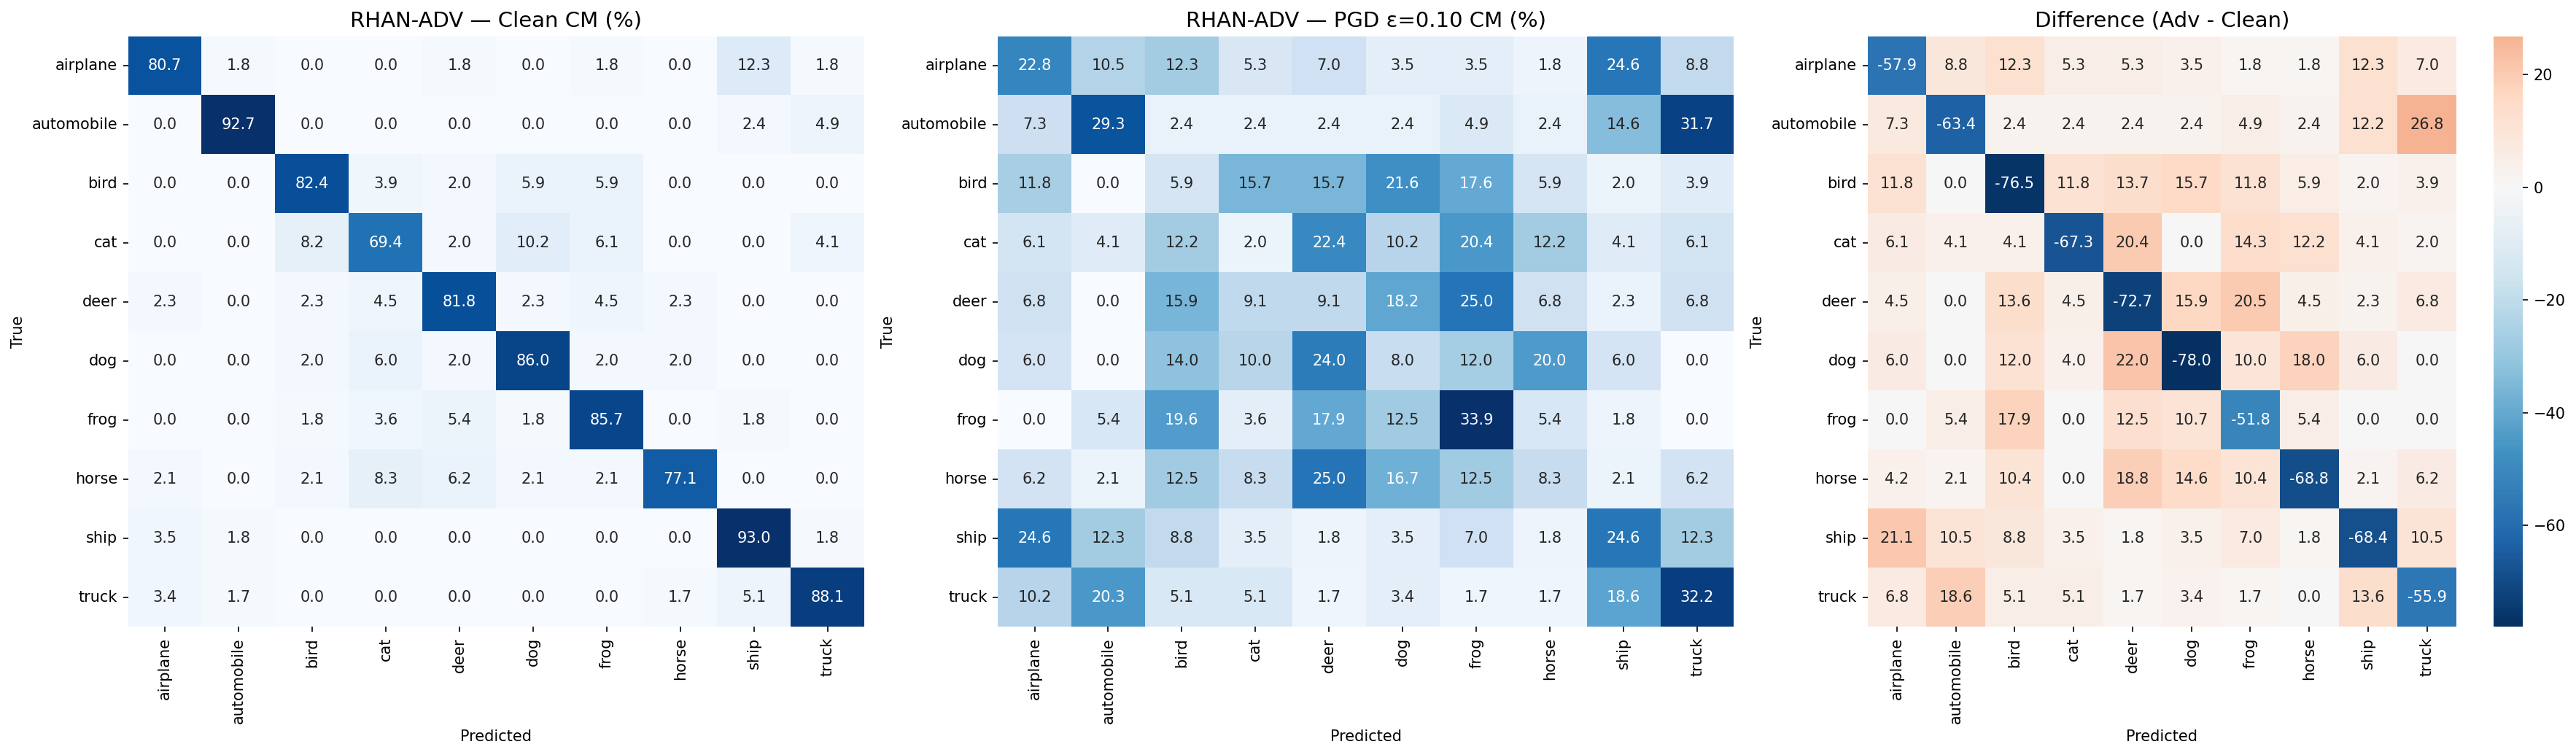
\includegraphics[width=\textwidth]{figures/rhan-adv_confusion_suite.png}
  \caption{RHAN-adv (Fig.~A.19).}
  \label{fig:rhan_adv_conf}
\end{subfigure}
\caption{\textbf{RHAN Confusion Suite Comparison}.}
\label{fig:rhan_conf_comparison}
\end{figure}

\subsection{Recurrent Feedback Gating Maps}

\begin{figure}[H]
\centering
\begin{subfigure}[b]{0.48\textwidth}
  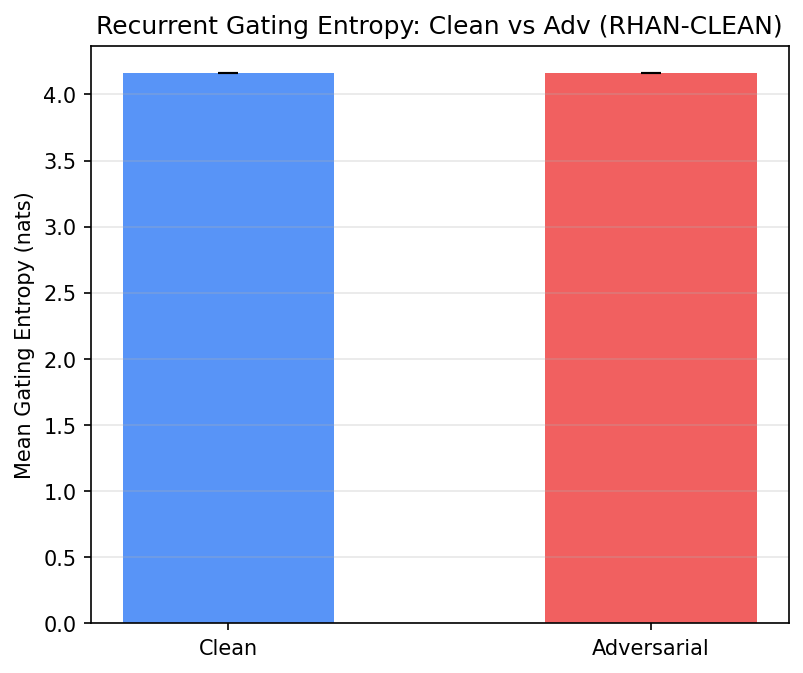
\includegraphics[width=\textwidth]{figures/gating_entropy_comparison.png}
  \caption{Gate Entropy (Fig.~A.20).}
  \label{fig:gate_entropy_comparison_app}
\end{subfigure}
\hfill
\begin{subfigure}[b]{0.48\textwidth}
  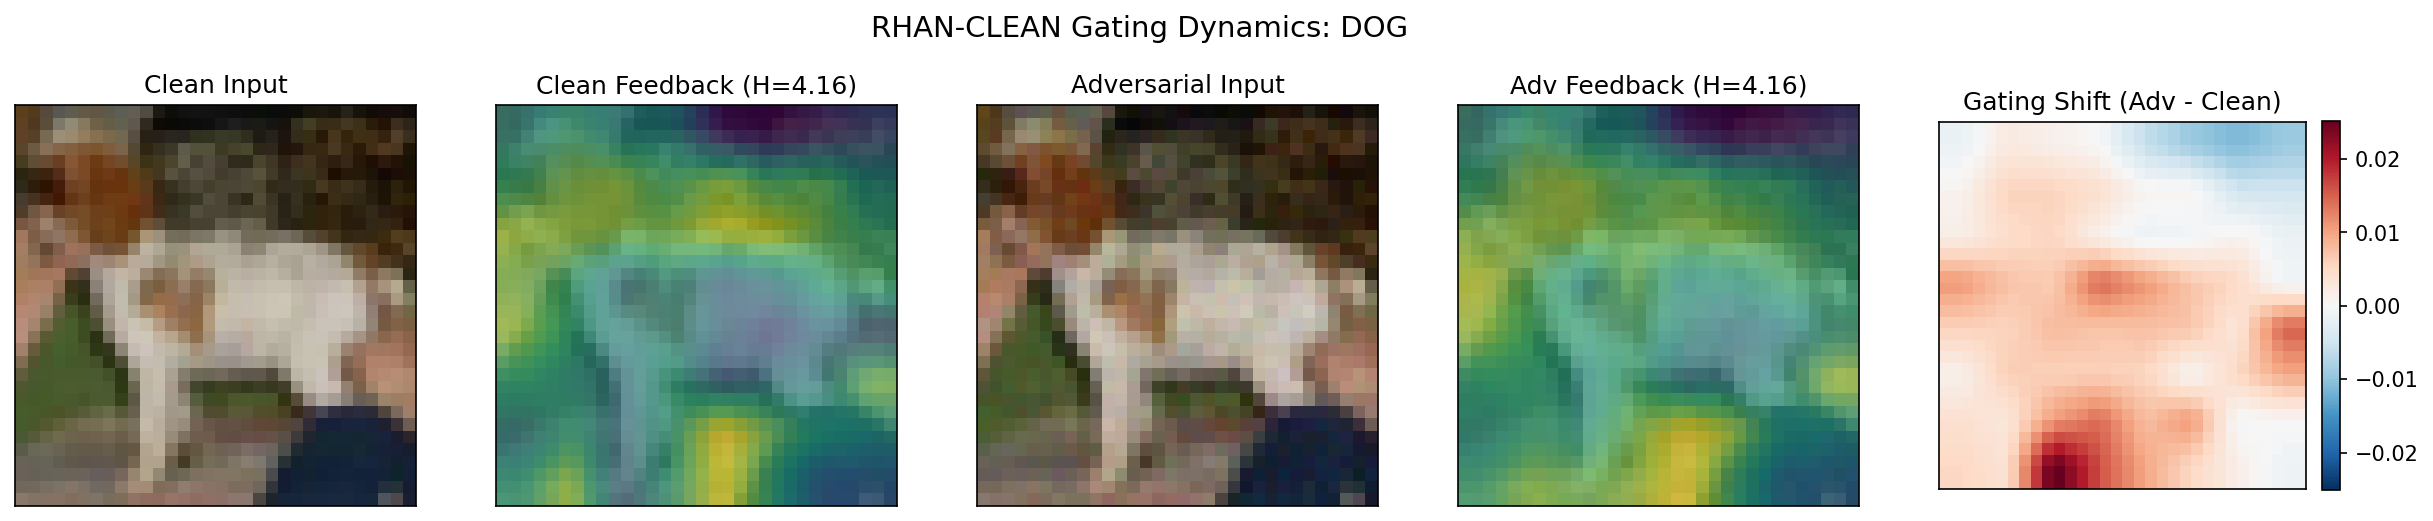
\includegraphics[width=\textwidth]{figures/feedback_dog.png}
  \caption{Dog Gating Map (Fig.~A.21).}
  \label{fig:feedback_dog_app}
\end{subfigure}
\caption{\textbf{RHAN-adv Gating Dynamics}.}
\label{fig:gating_dynamics_app}
\end{figure}

\begin{figure}[H]
\centering
\begin{subfigure}[b]{0.48\textwidth}
  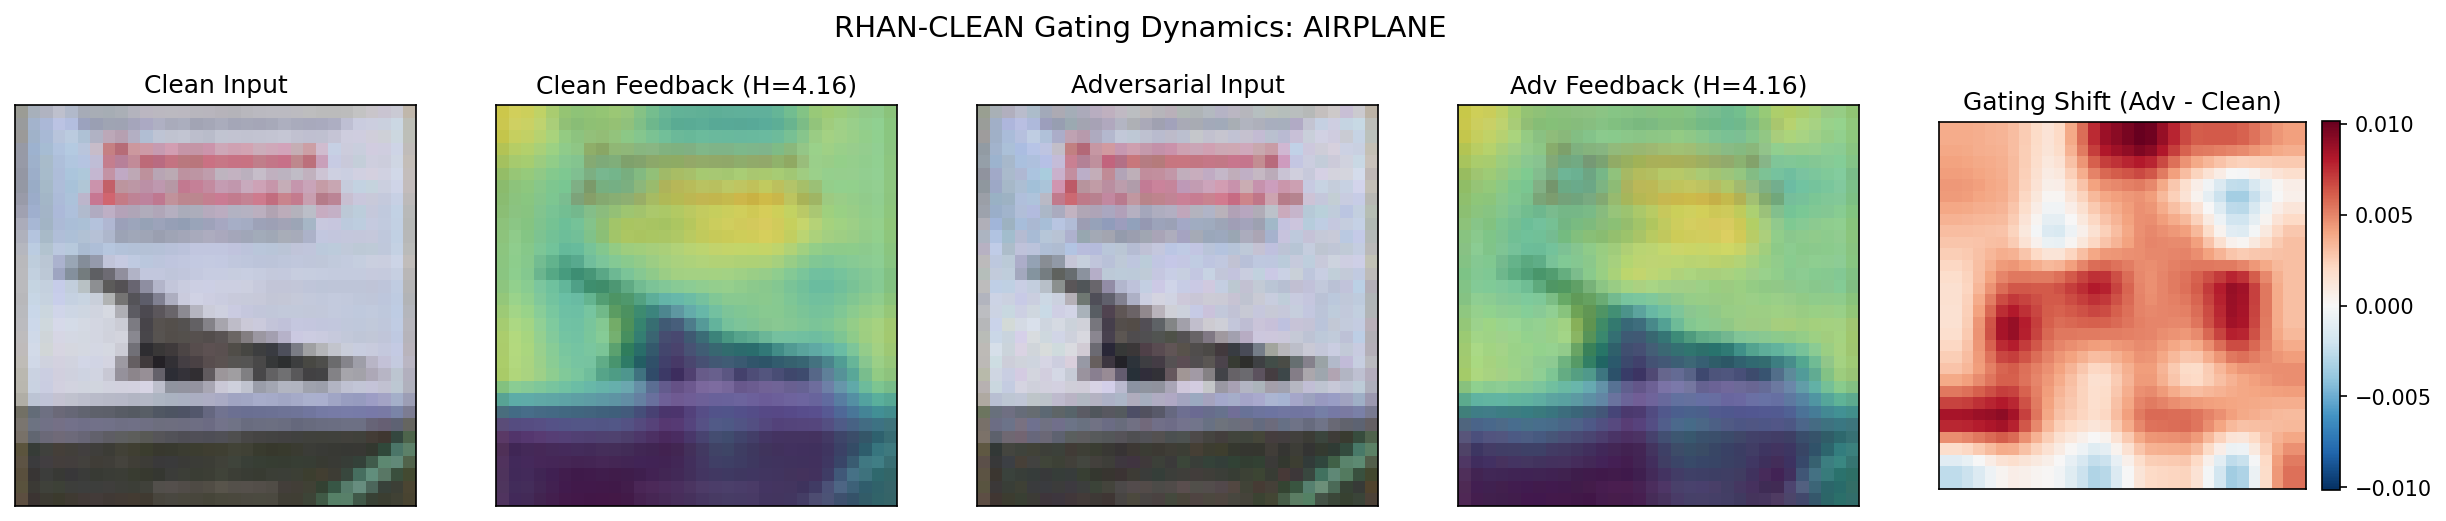
\includegraphics[width=\textwidth]{figures/feedback_airplane.png}
  \caption{Airplane (Fig.~A.22).}
  \label{fig:feedback_airplane}
\end{subfigure}
\hfill
\begin{subfigure}[b]{0.48\textwidth}
  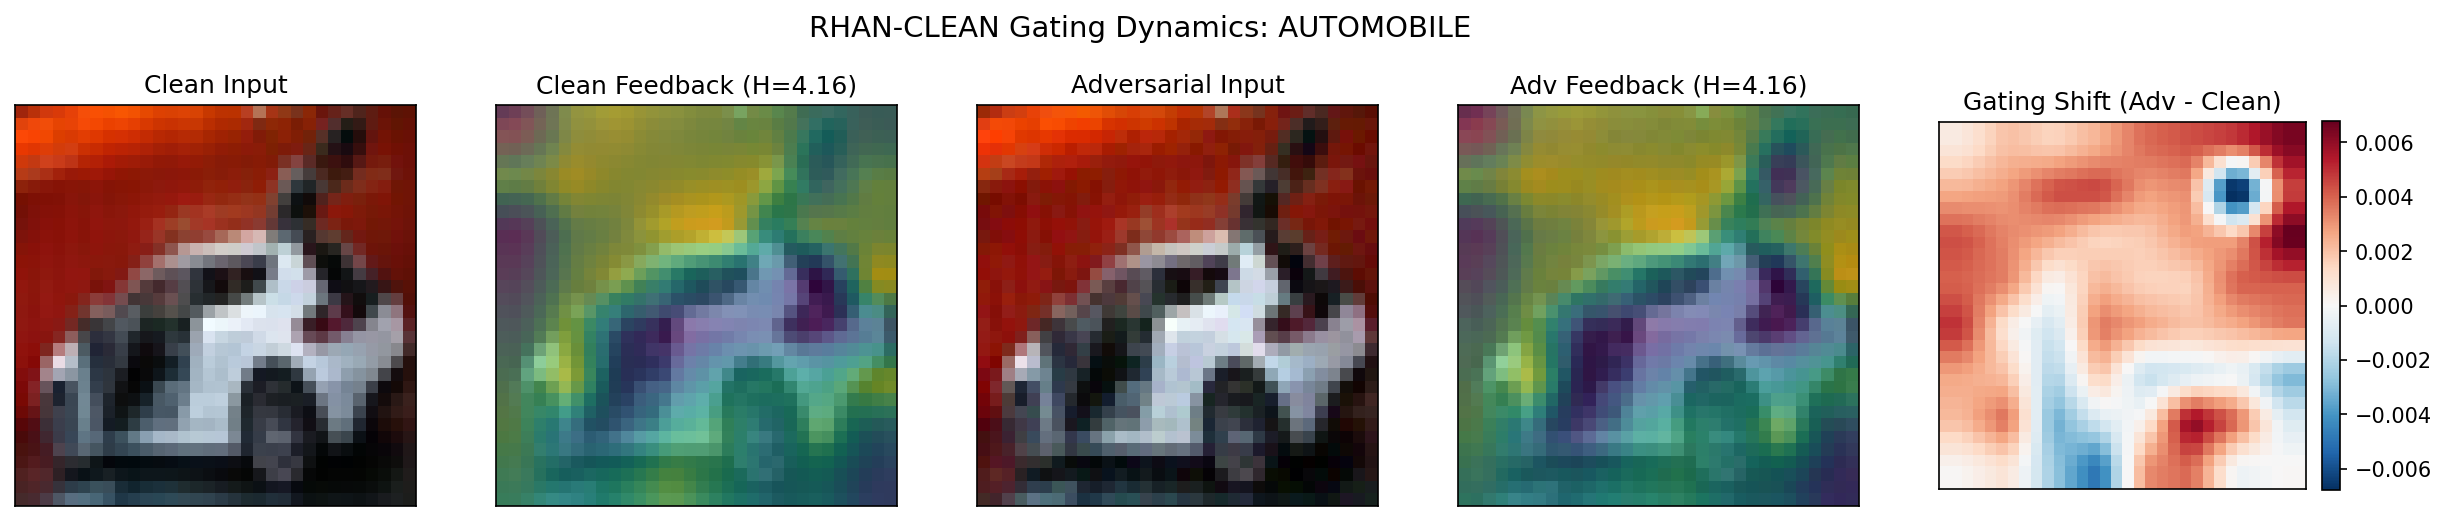
\includegraphics[width=\textwidth]{figures/feedback_automobile.png}
  \caption{Automobile (Fig.~A.23).}
  \label{fig:feedback_automobile}
\end{subfigure}
\caption{\textbf{Gating Maps: Airplane and Automobile}.}
\label{fig:gating_airplane_auto}
\end{figure}

\begin{figure}[H]
\centering
\begin{subfigure}[b]{0.48\textwidth}
  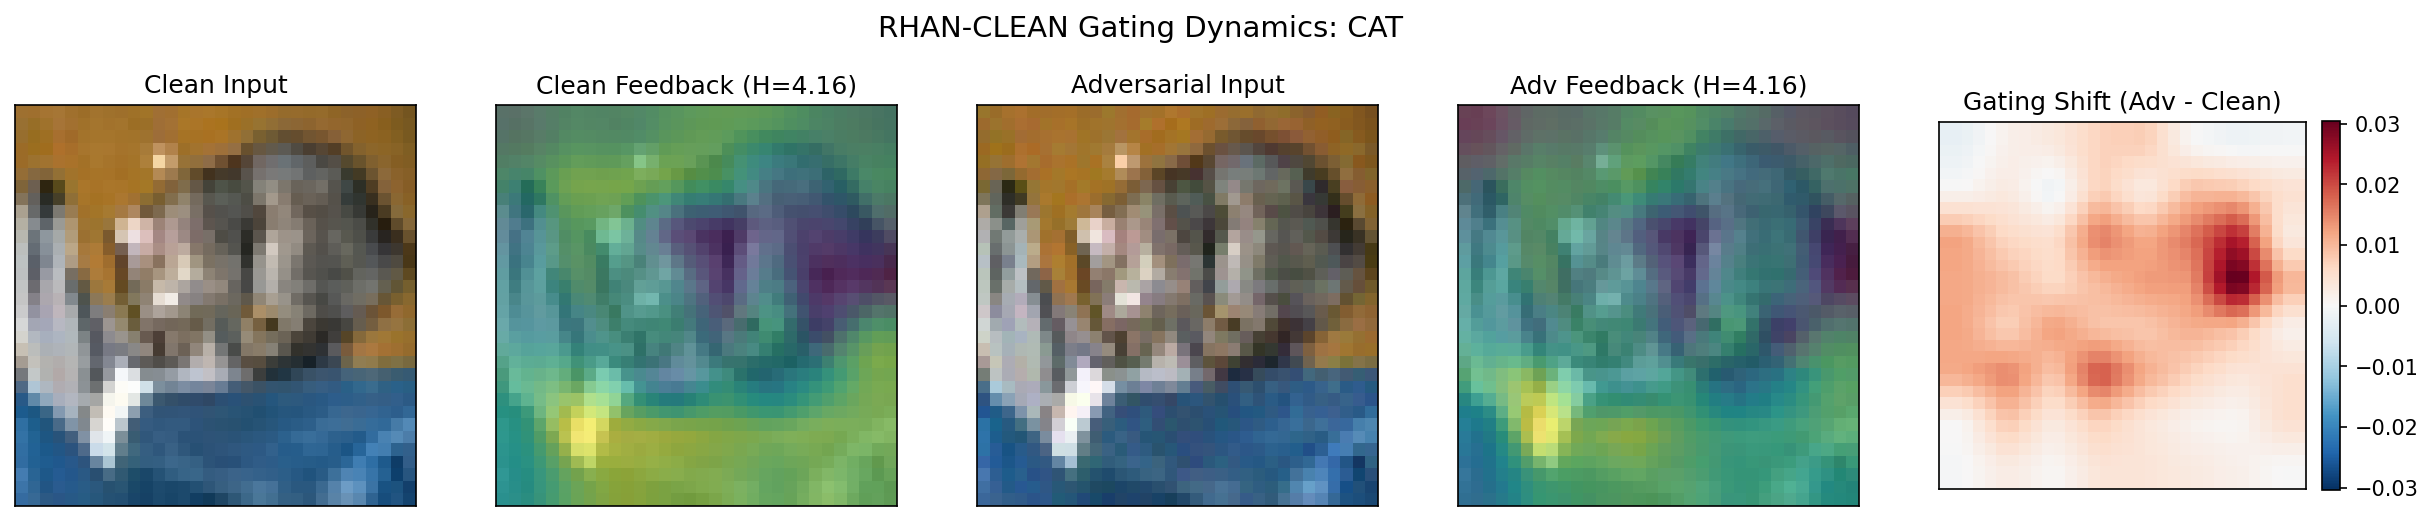
\includegraphics[width=\textwidth]{figures/feedback_cat.png}
  \caption{Cat (Fig.~A.24).}
  \label{fig:feedback_cat}
\end{subfigure}
\hfill
\begin{subfigure}[b]{0.48\textwidth}
  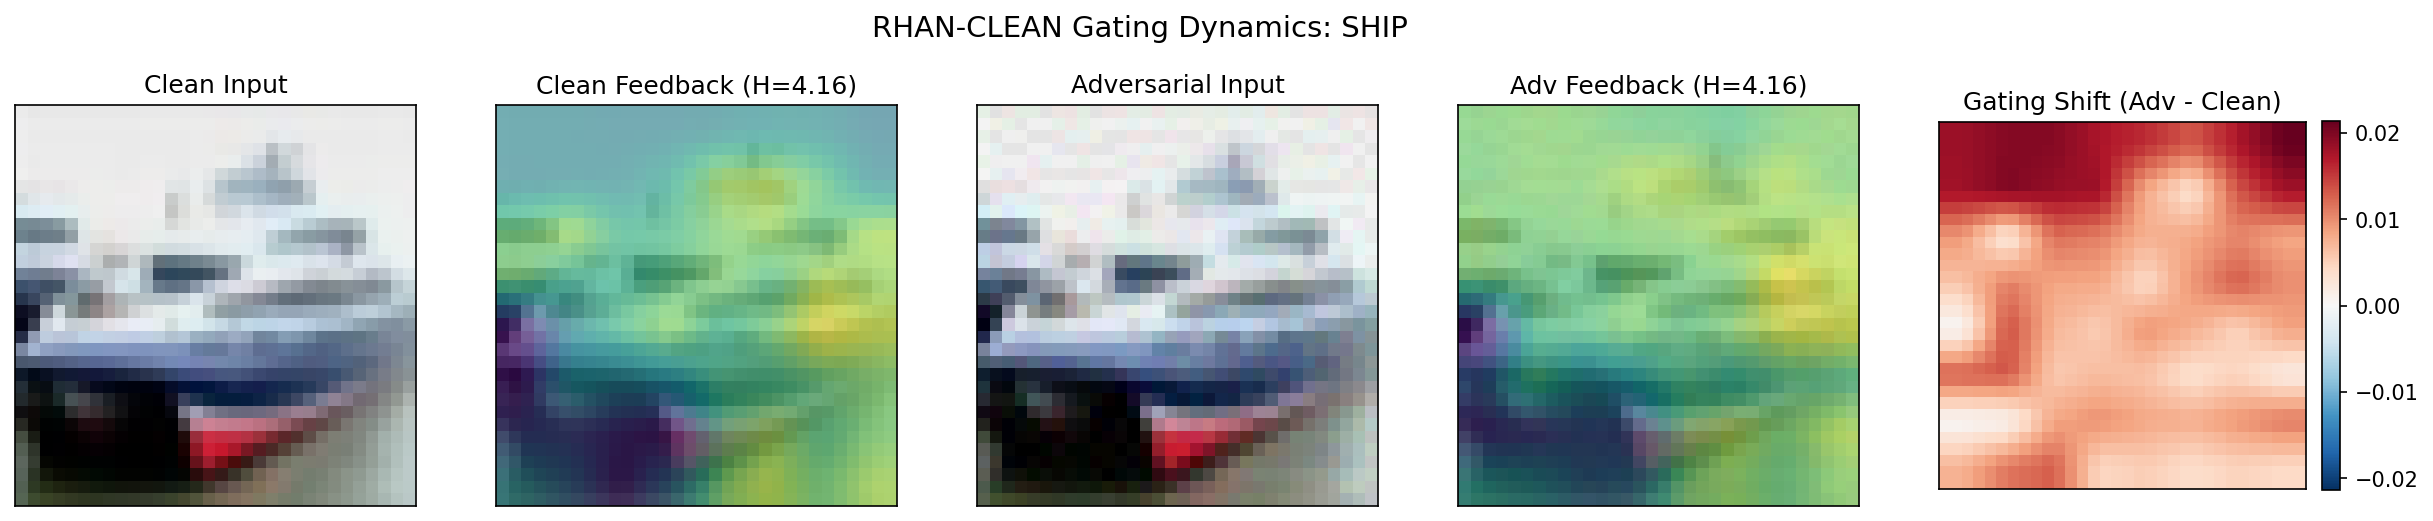
\includegraphics[width=\textwidth]{figures/feedback_ship.png}
  \caption{Ship (Fig.~A.25).}
  \label{fig:feedback_ship}
\end{subfigure}
\caption{\textbf{Gating Maps: Cat and Ship}.}
\label{fig:gating_cat_ship}
\end{figure}

\subsection{Visual Psychophysics Stimuli and Grad-CAM Explanations}

\begin{figure}[H]
\centering
\begin{subfigure}[b]{0.32\textwidth}
  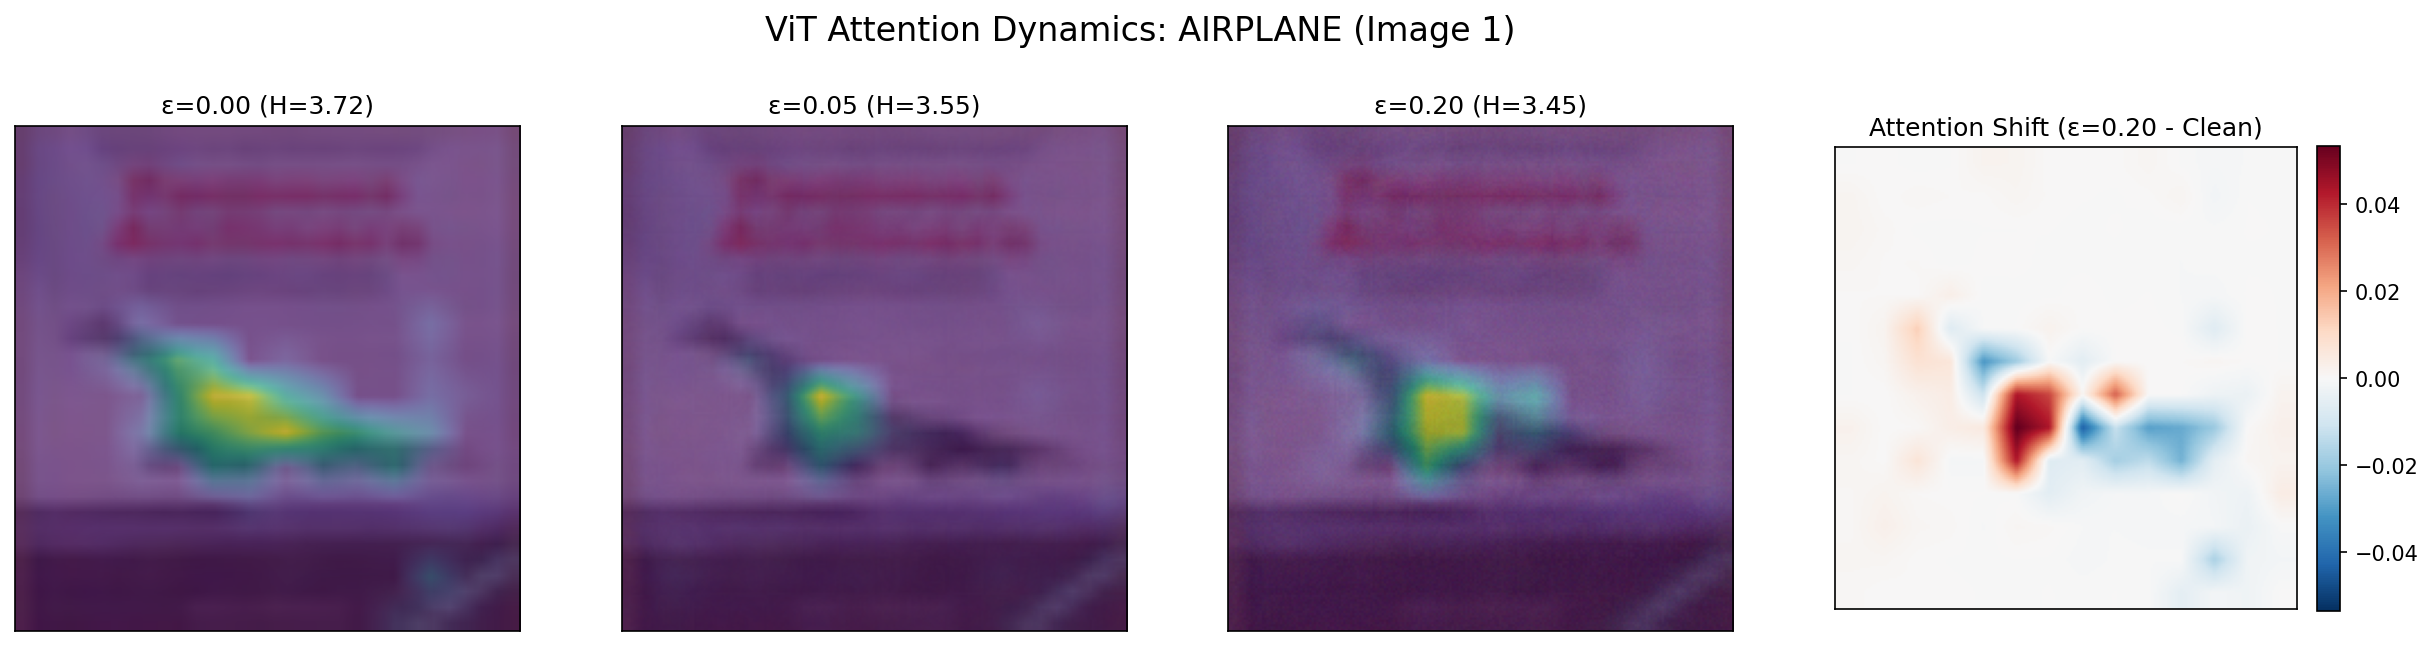
\includegraphics[width=\textwidth]{figures/airplane_1.png}
  \caption{Clean}
  \label{fig:air_clean}
\end{subfigure}
\hfill
\begin{subfigure}[b]{0.32\textwidth}
  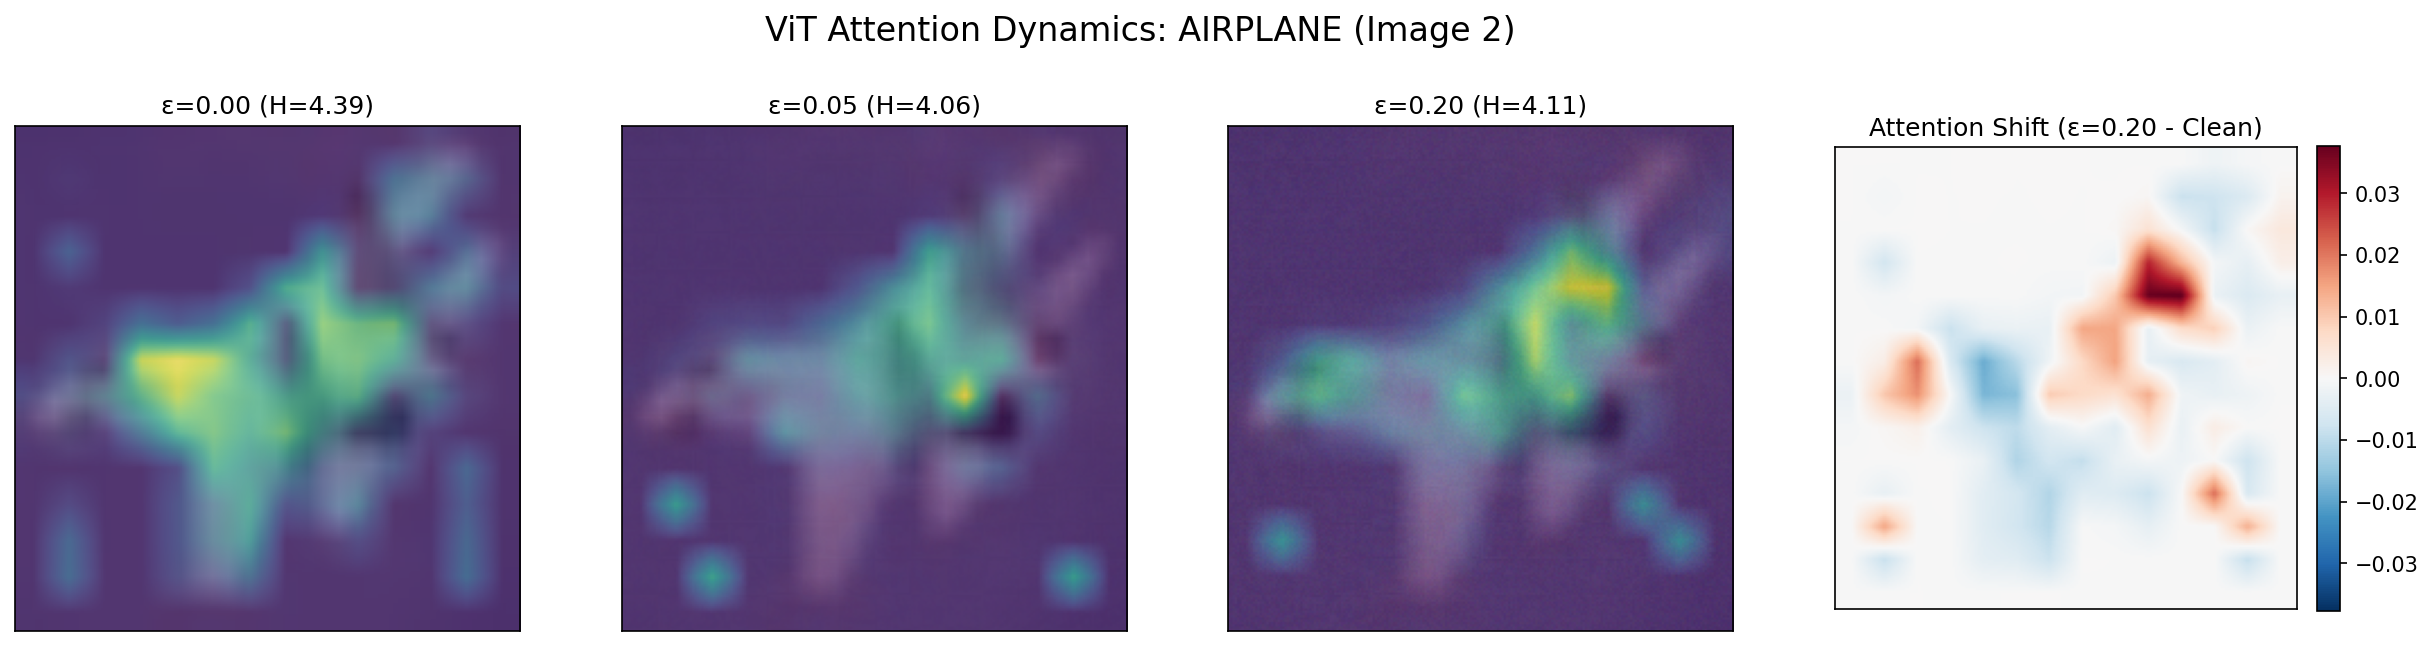
\includegraphics[width=\textwidth]{figures/airplane_2.png}
  \caption{Adversarial}
  \label{fig:air_adv}
\end{subfigure}
\hfill
\begin{subfigure}[b]{0.32\textwidth}
  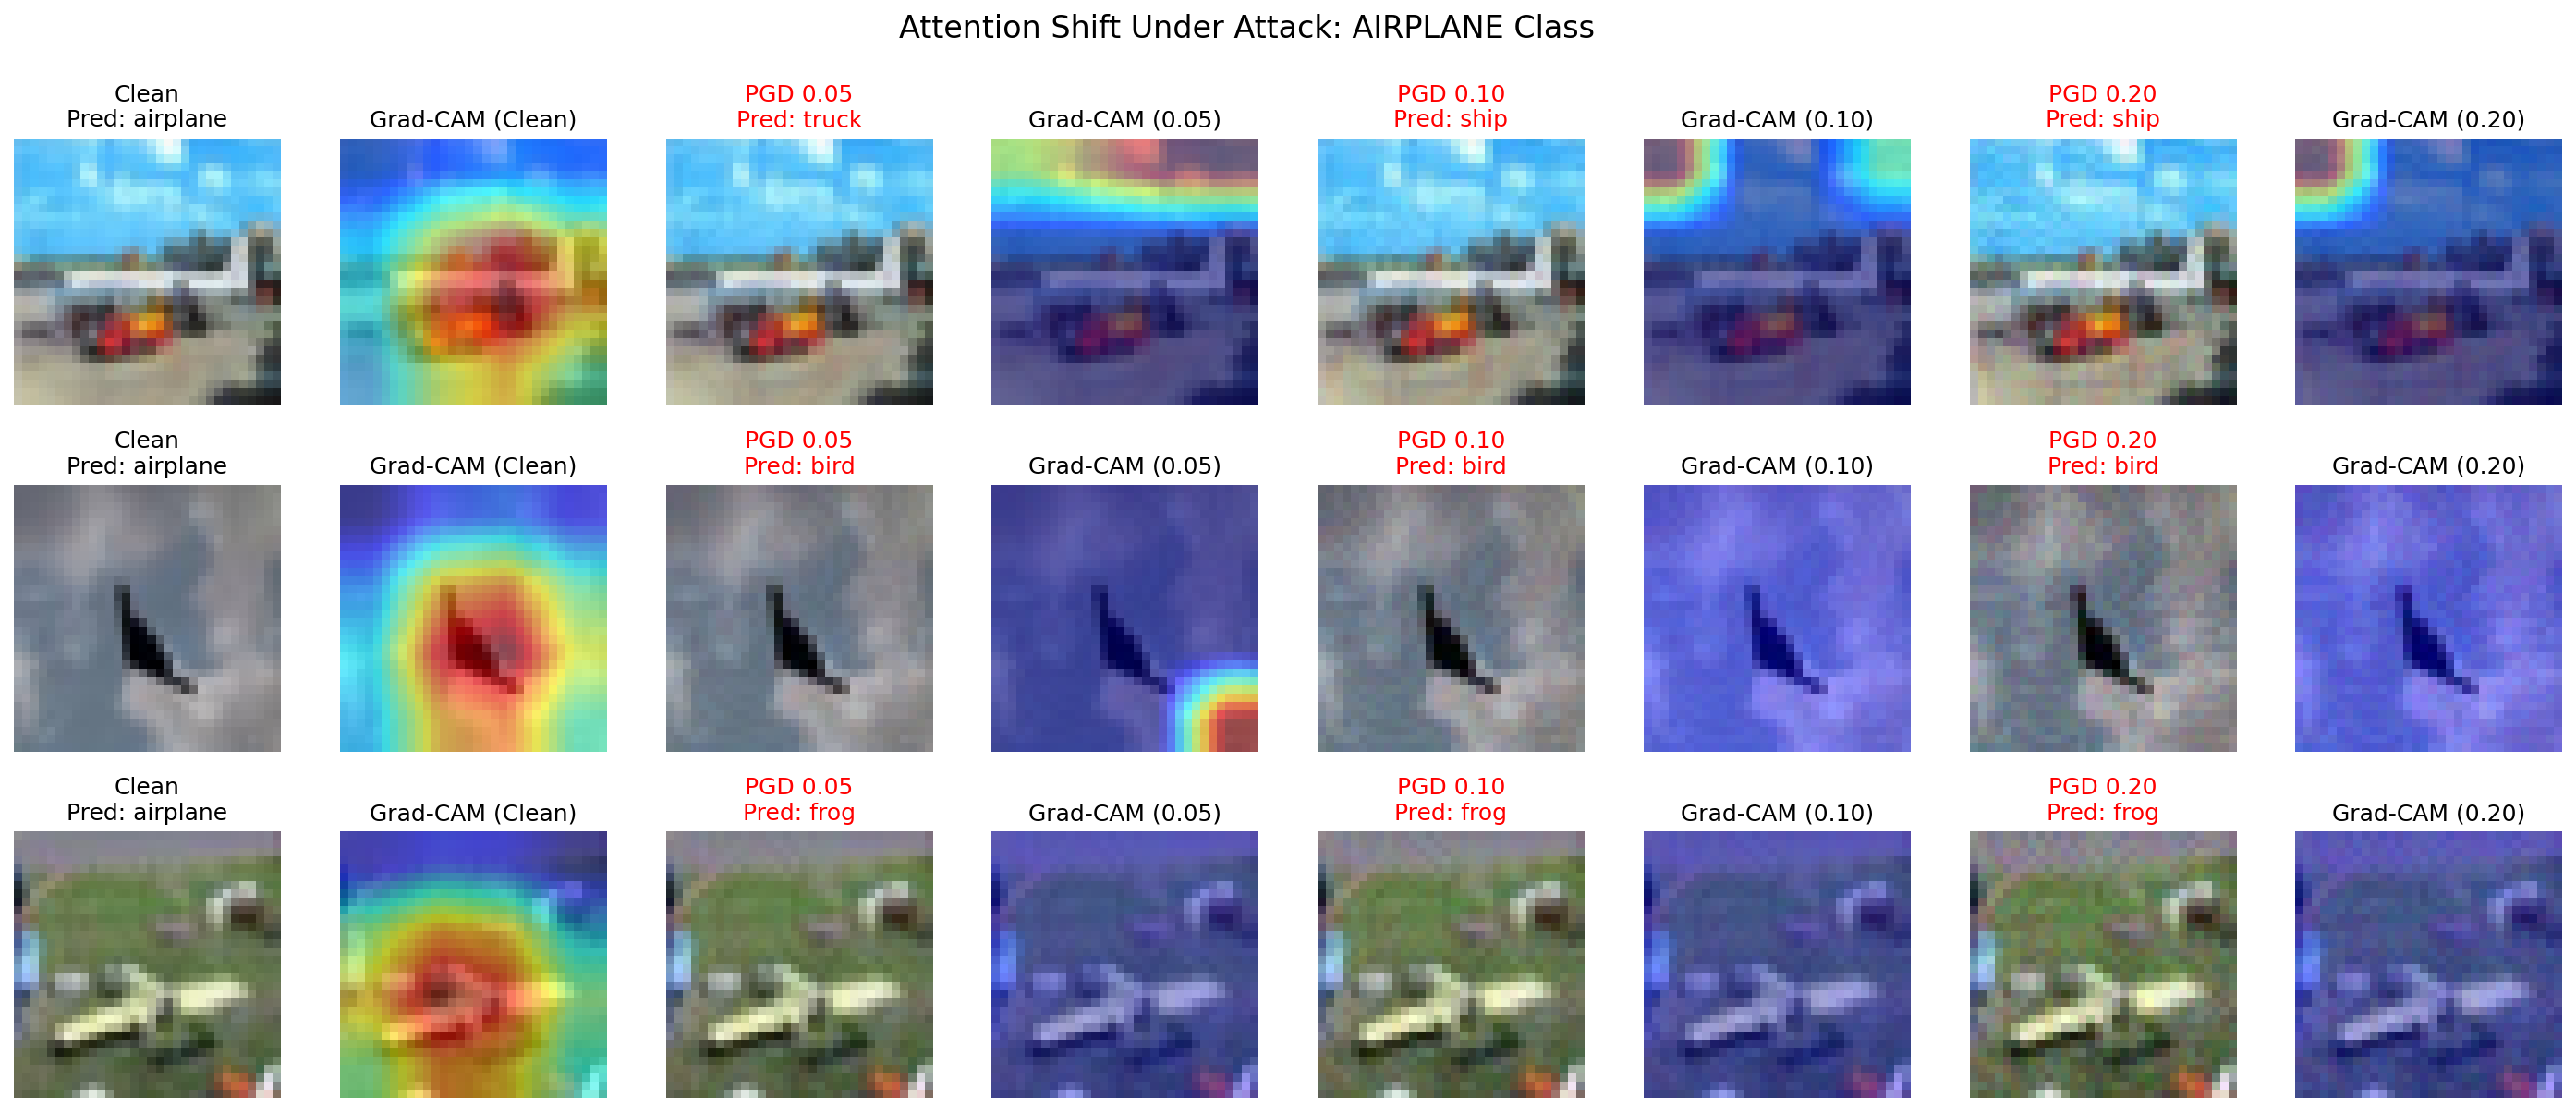
\includegraphics[width=\textwidth]{figures/airplane_gradcam.png}
  \caption{Grad-CAM}
  \label{fig:air_grad}
\end{subfigure}
\caption{\textbf{Airplane Stimuli and Grad-CAM (Fig.~A.26, A.27)}.}
\label{fig:stim_airplane}
\end{figure}

\begin{figure}[H]
\centering
\begin{subfigure}[b]{0.32\textwidth}
  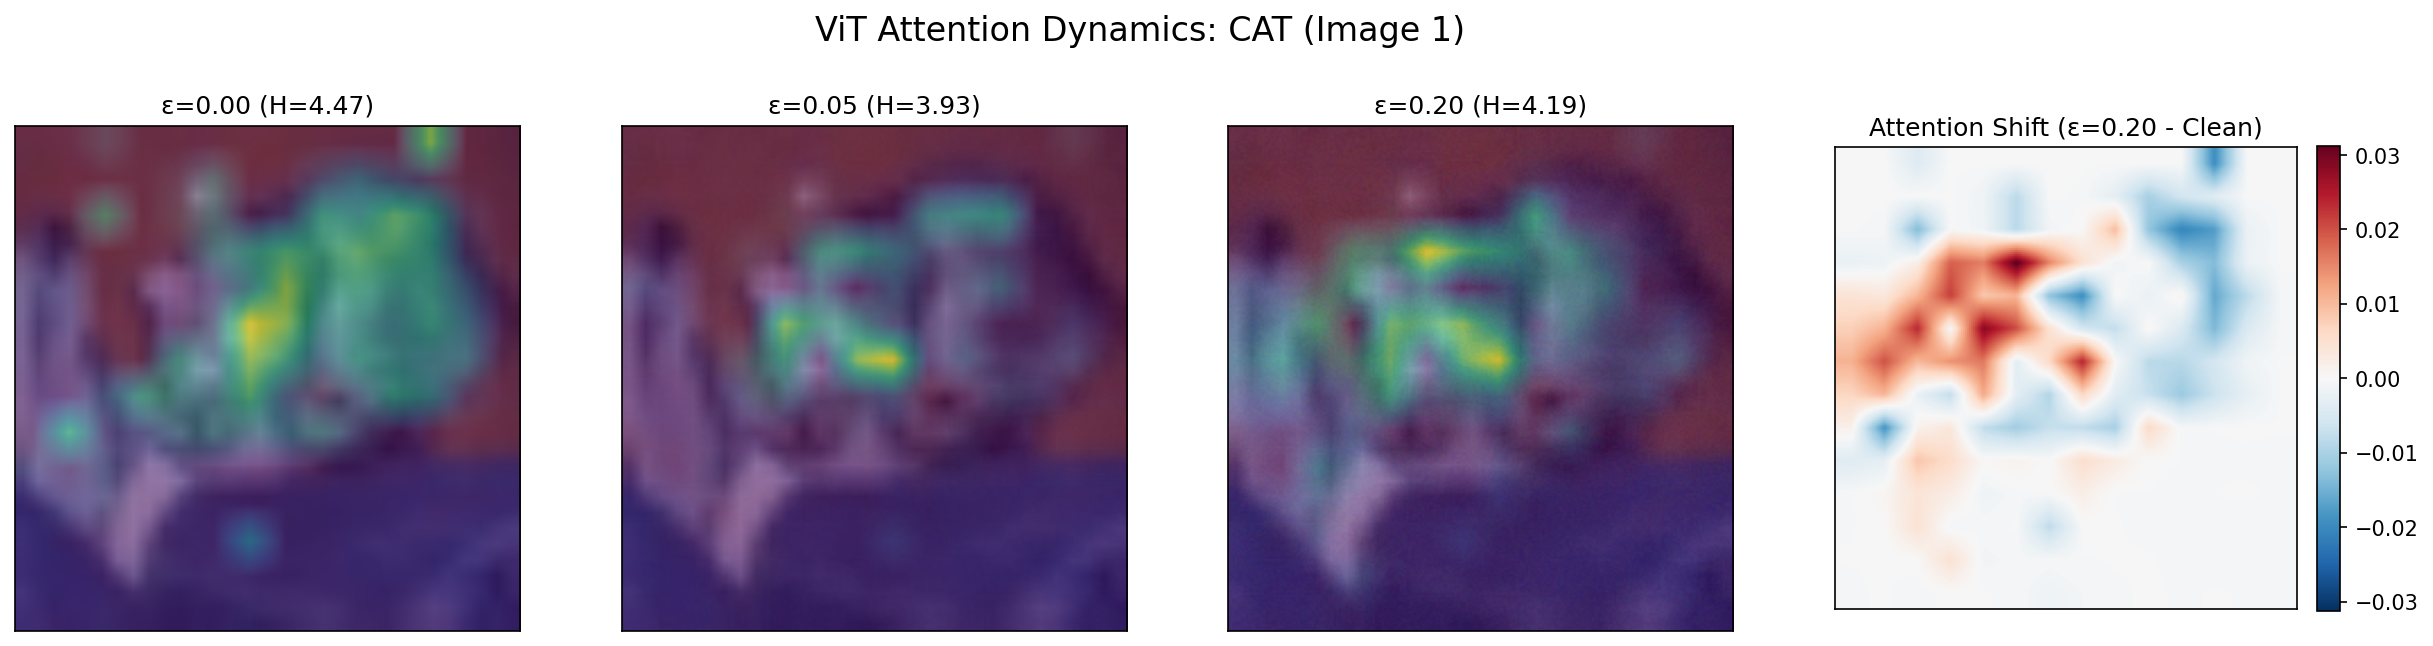
\includegraphics[width=\textwidth]{figures/cat_1.png}
  \caption{Clean}
  \label{fig:cat_clean_stim}
\end{subfigure}
\hfill
\begin{subfigure}[b]{0.32\textwidth}
  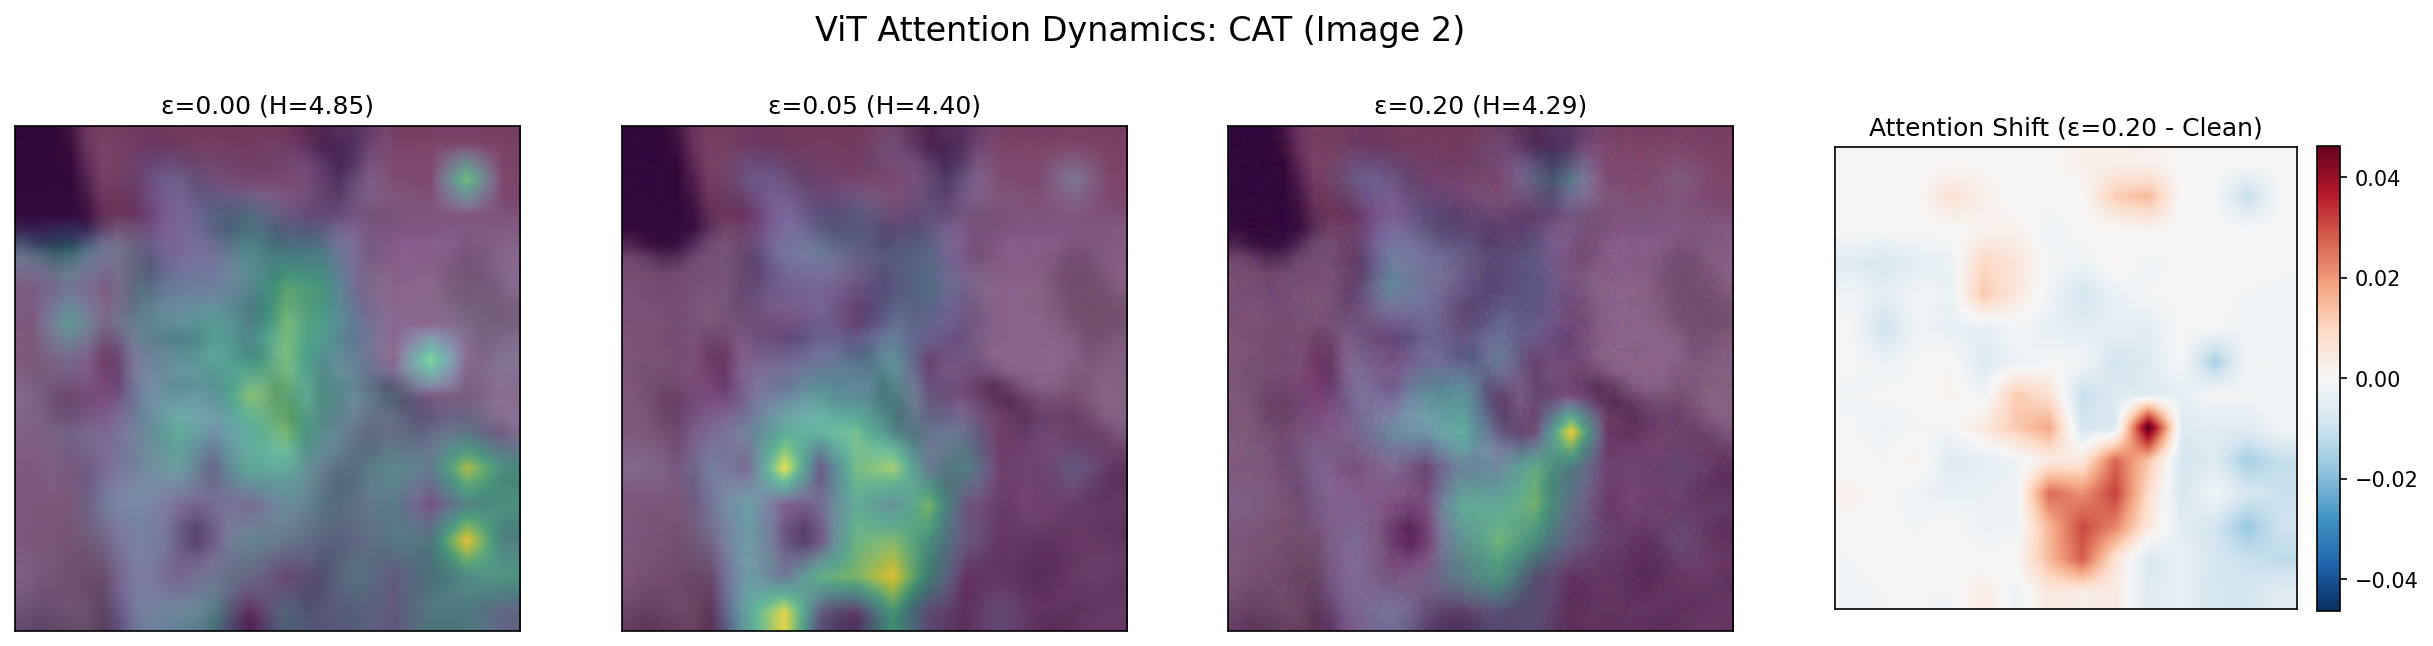
\includegraphics[width=\textwidth]{figures/cat_2.png}
  \caption{Adversarial}
  \label{fig:cat_adv_stim}
\end{subfigure}
\hfill
\begin{subfigure}[b]{0.32\textwidth}
  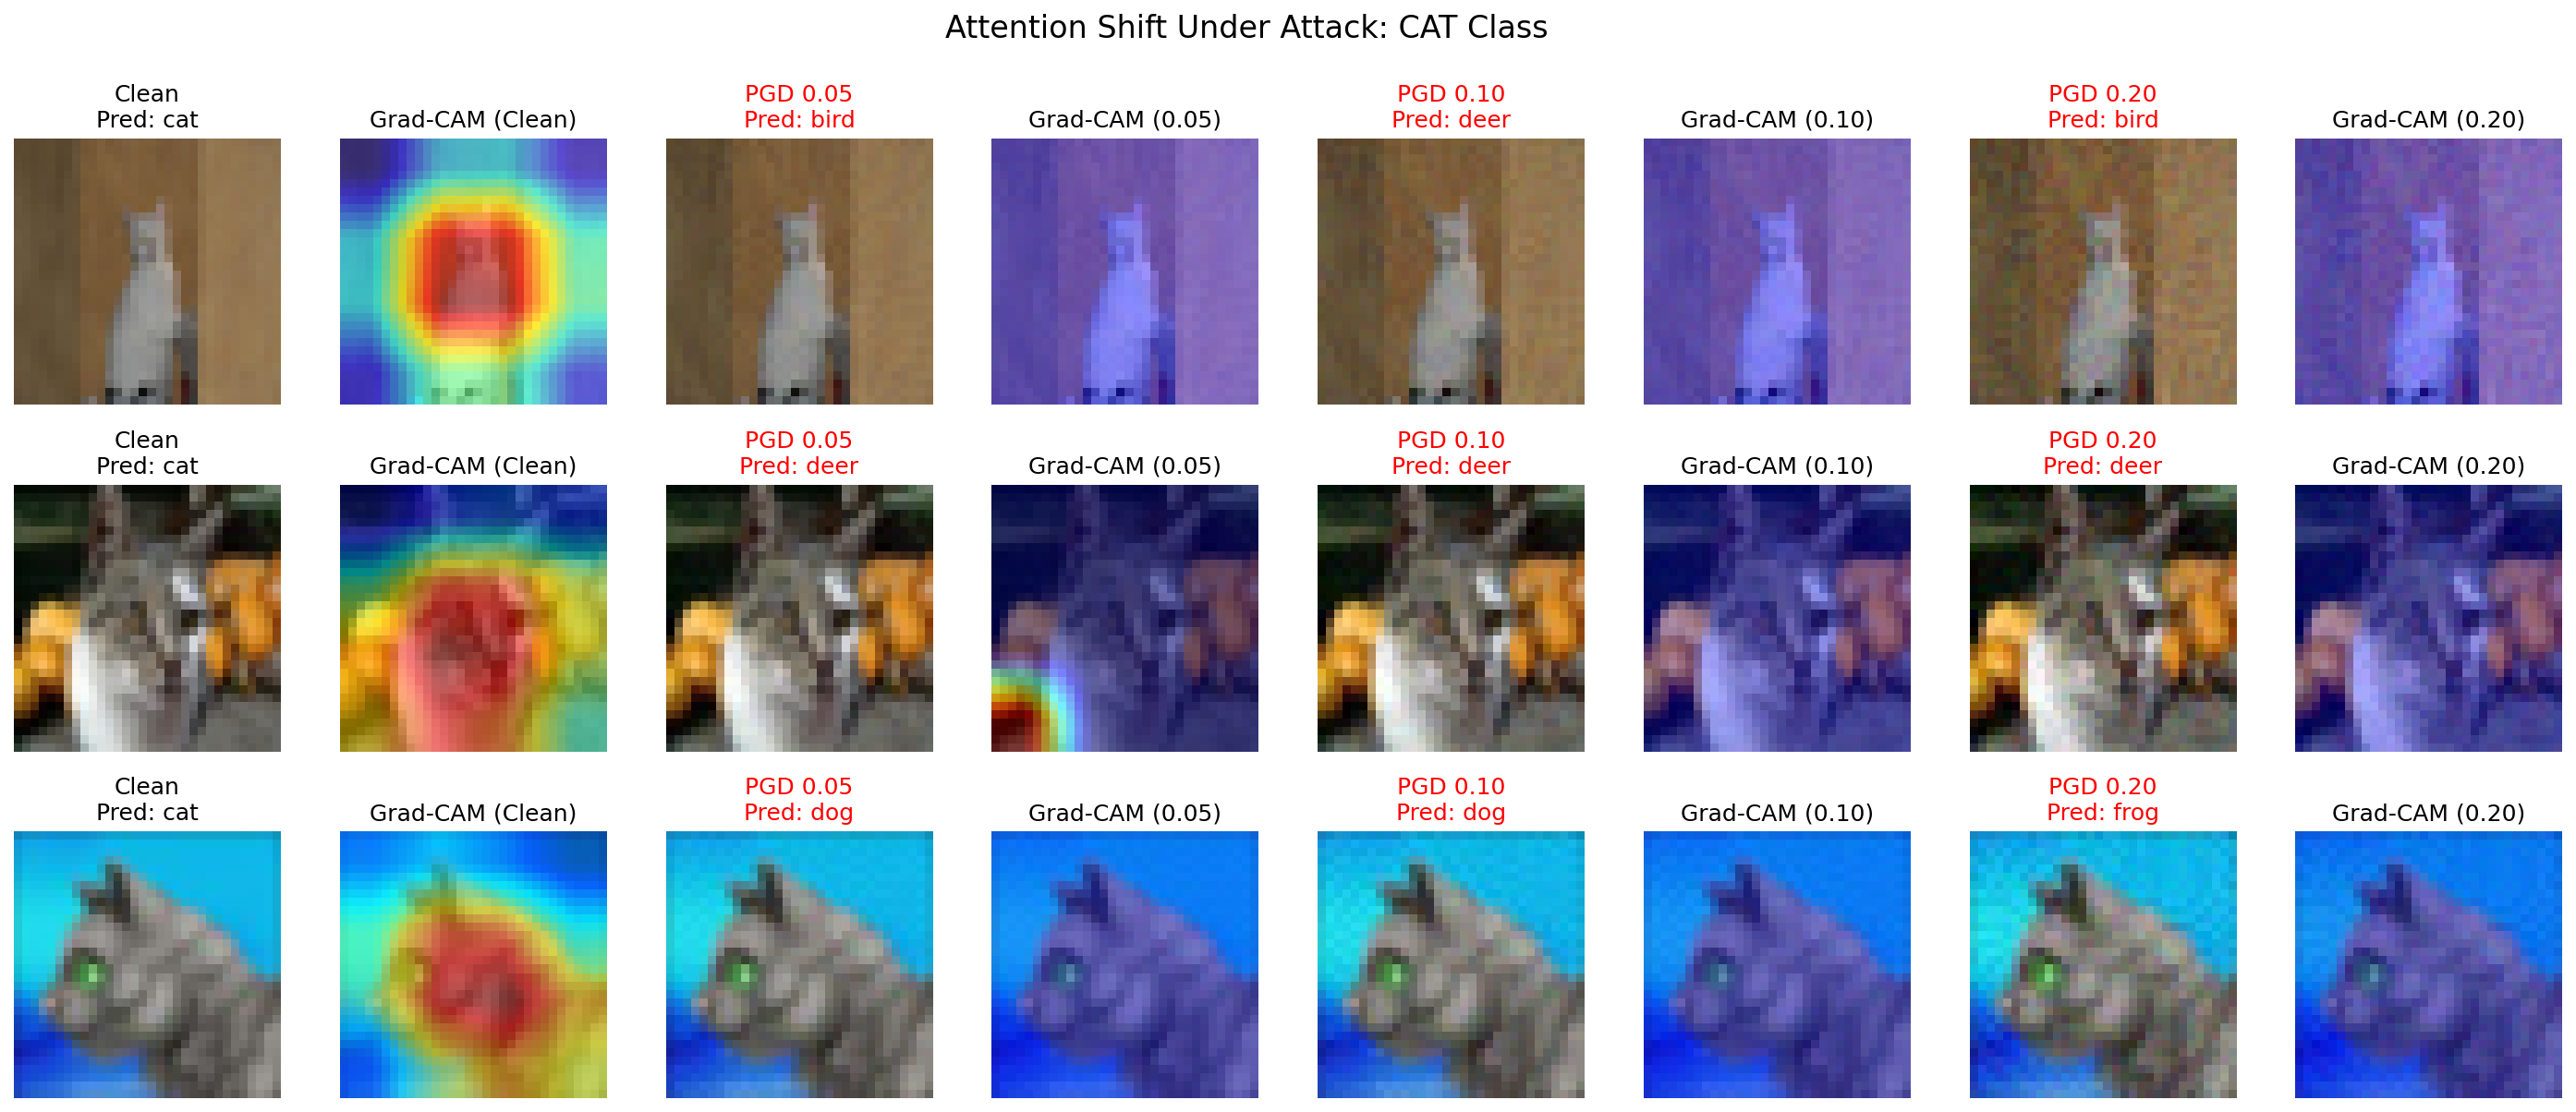
\includegraphics[width=\textwidth]{figures/cat_gradcam.png}
  \caption{Grad-CAM}
  \label{fig:cat_grad_cam}
\end{subfigure}
\caption{\textbf{Cat Stimuli and Grad-CAM (Fig.~A.28, A.29)}.}
\label{fig:stim_cat}
\end{figure}

\begin{figure}[H]
\centering
\begin{subfigure}[b]{0.32\textwidth}
  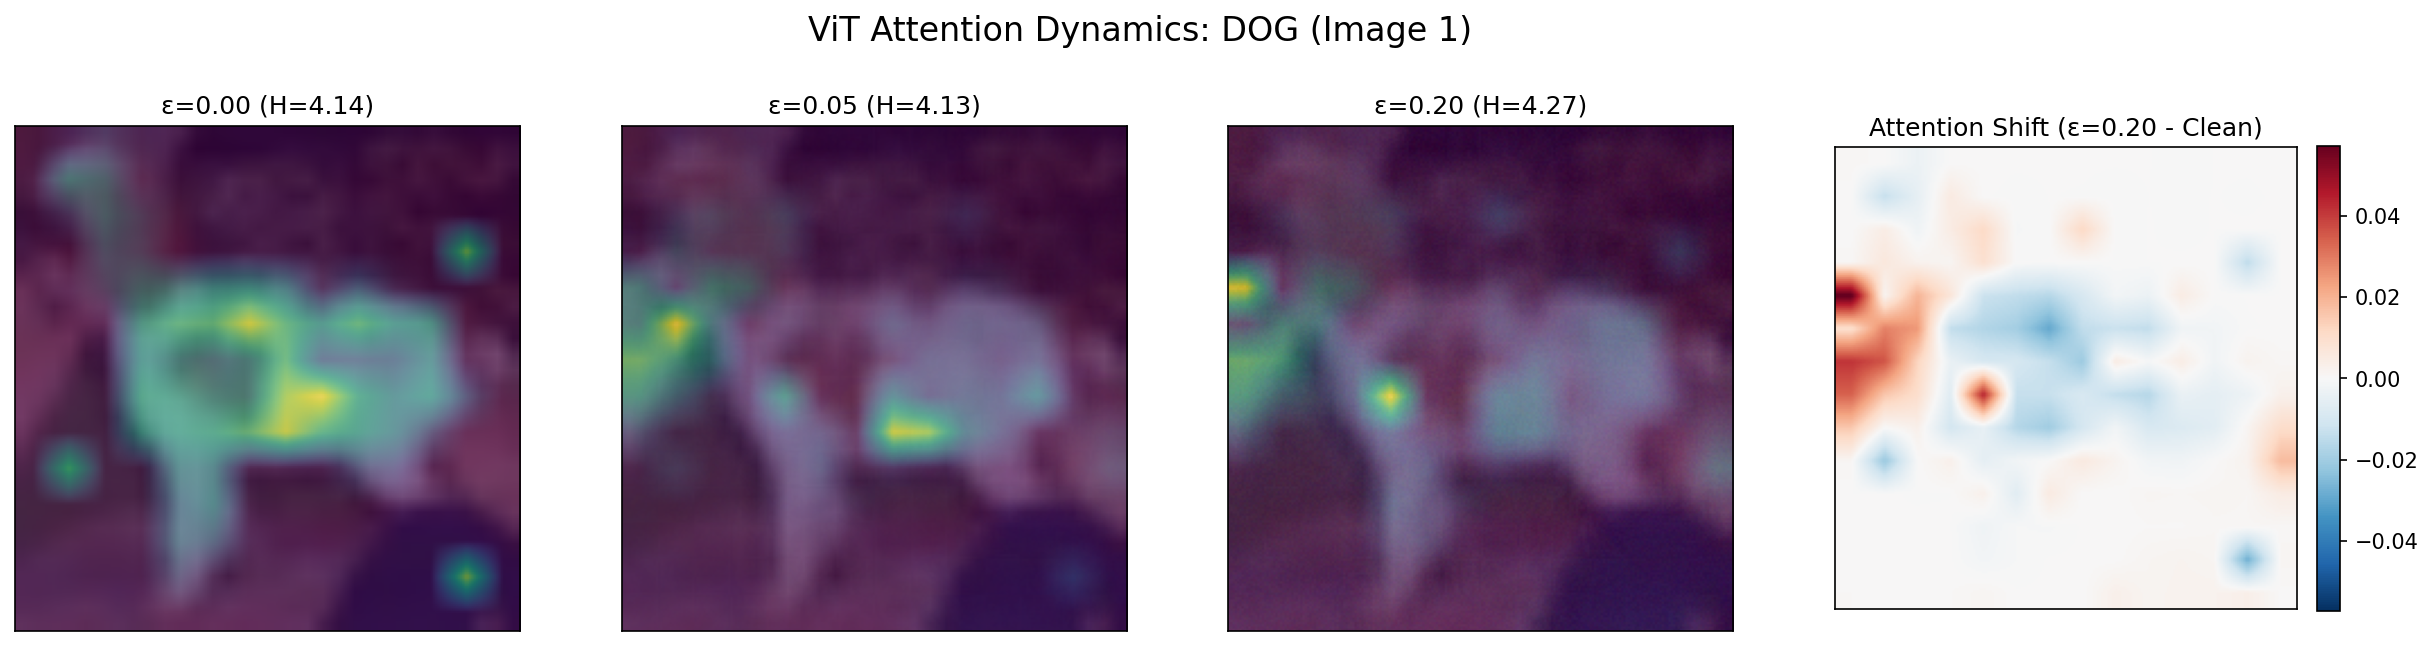
\includegraphics[width=\textwidth]{figures/dog_1.png}
  \caption{Clean}
  \label{fig:dog_clean_stim}
\end{subfigure}
\hfill
\begin{subfigure}[b]{0.32\textwidth}
  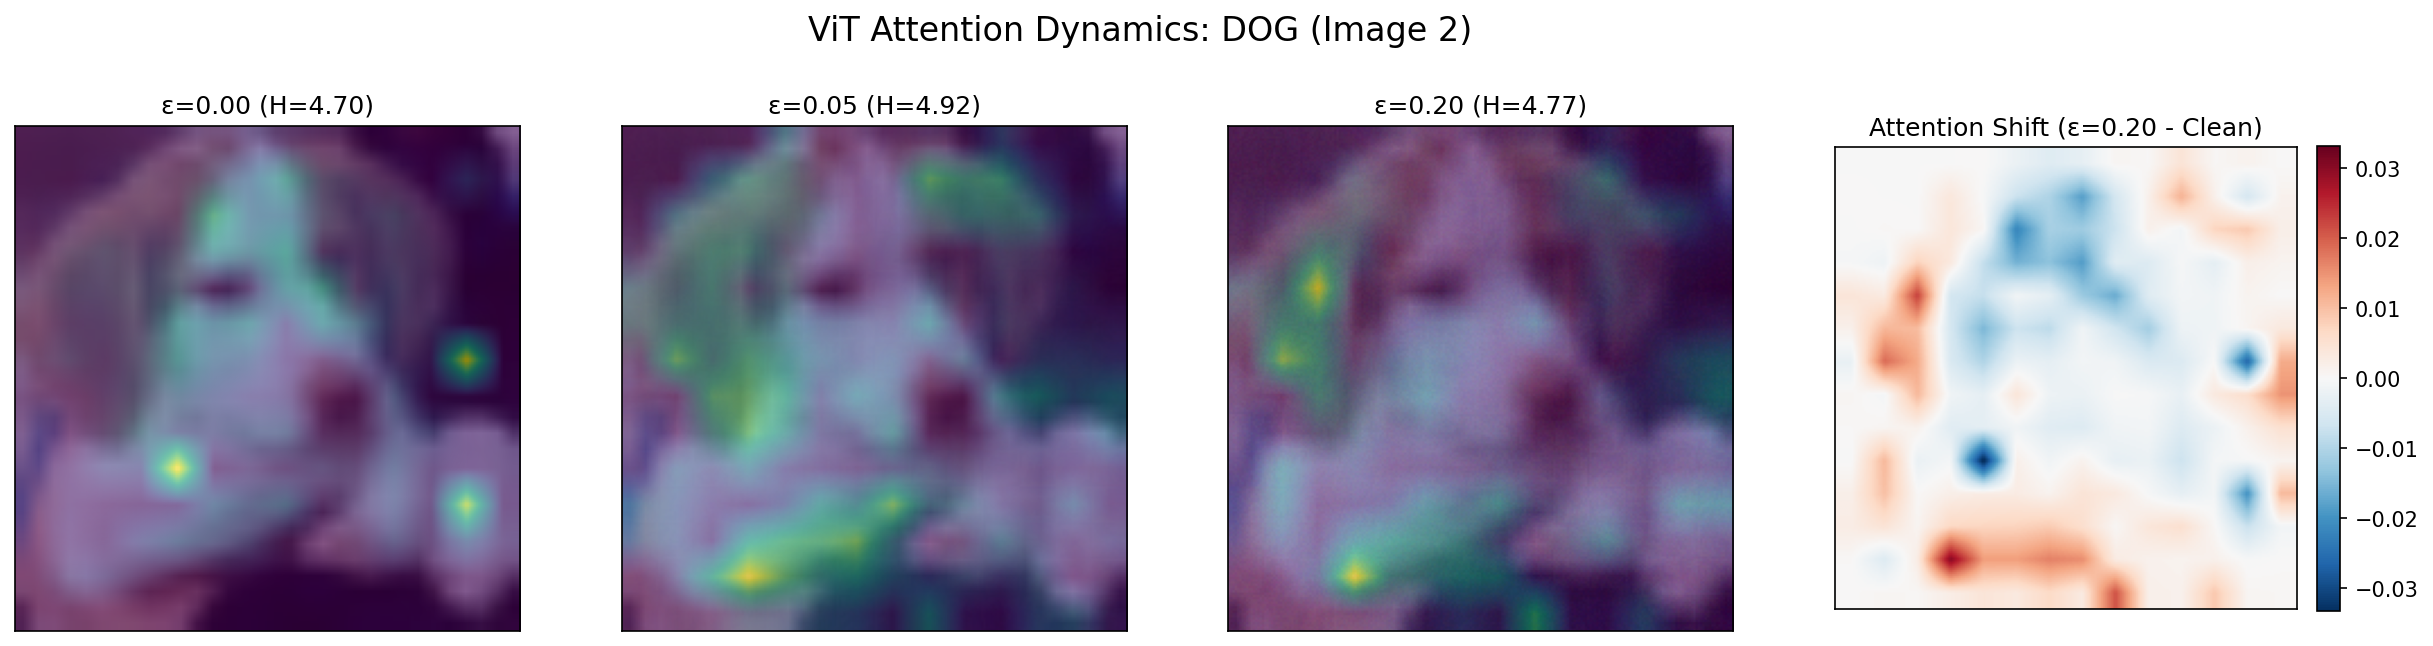
\includegraphics[width=\textwidth]{figures/dog_2.png}
  \caption{Adversarial}
  \label{fig:dog_adv_stim}
\end{subfigure}
\hfill
\begin{subfigure}[b]{0.32\textwidth}
  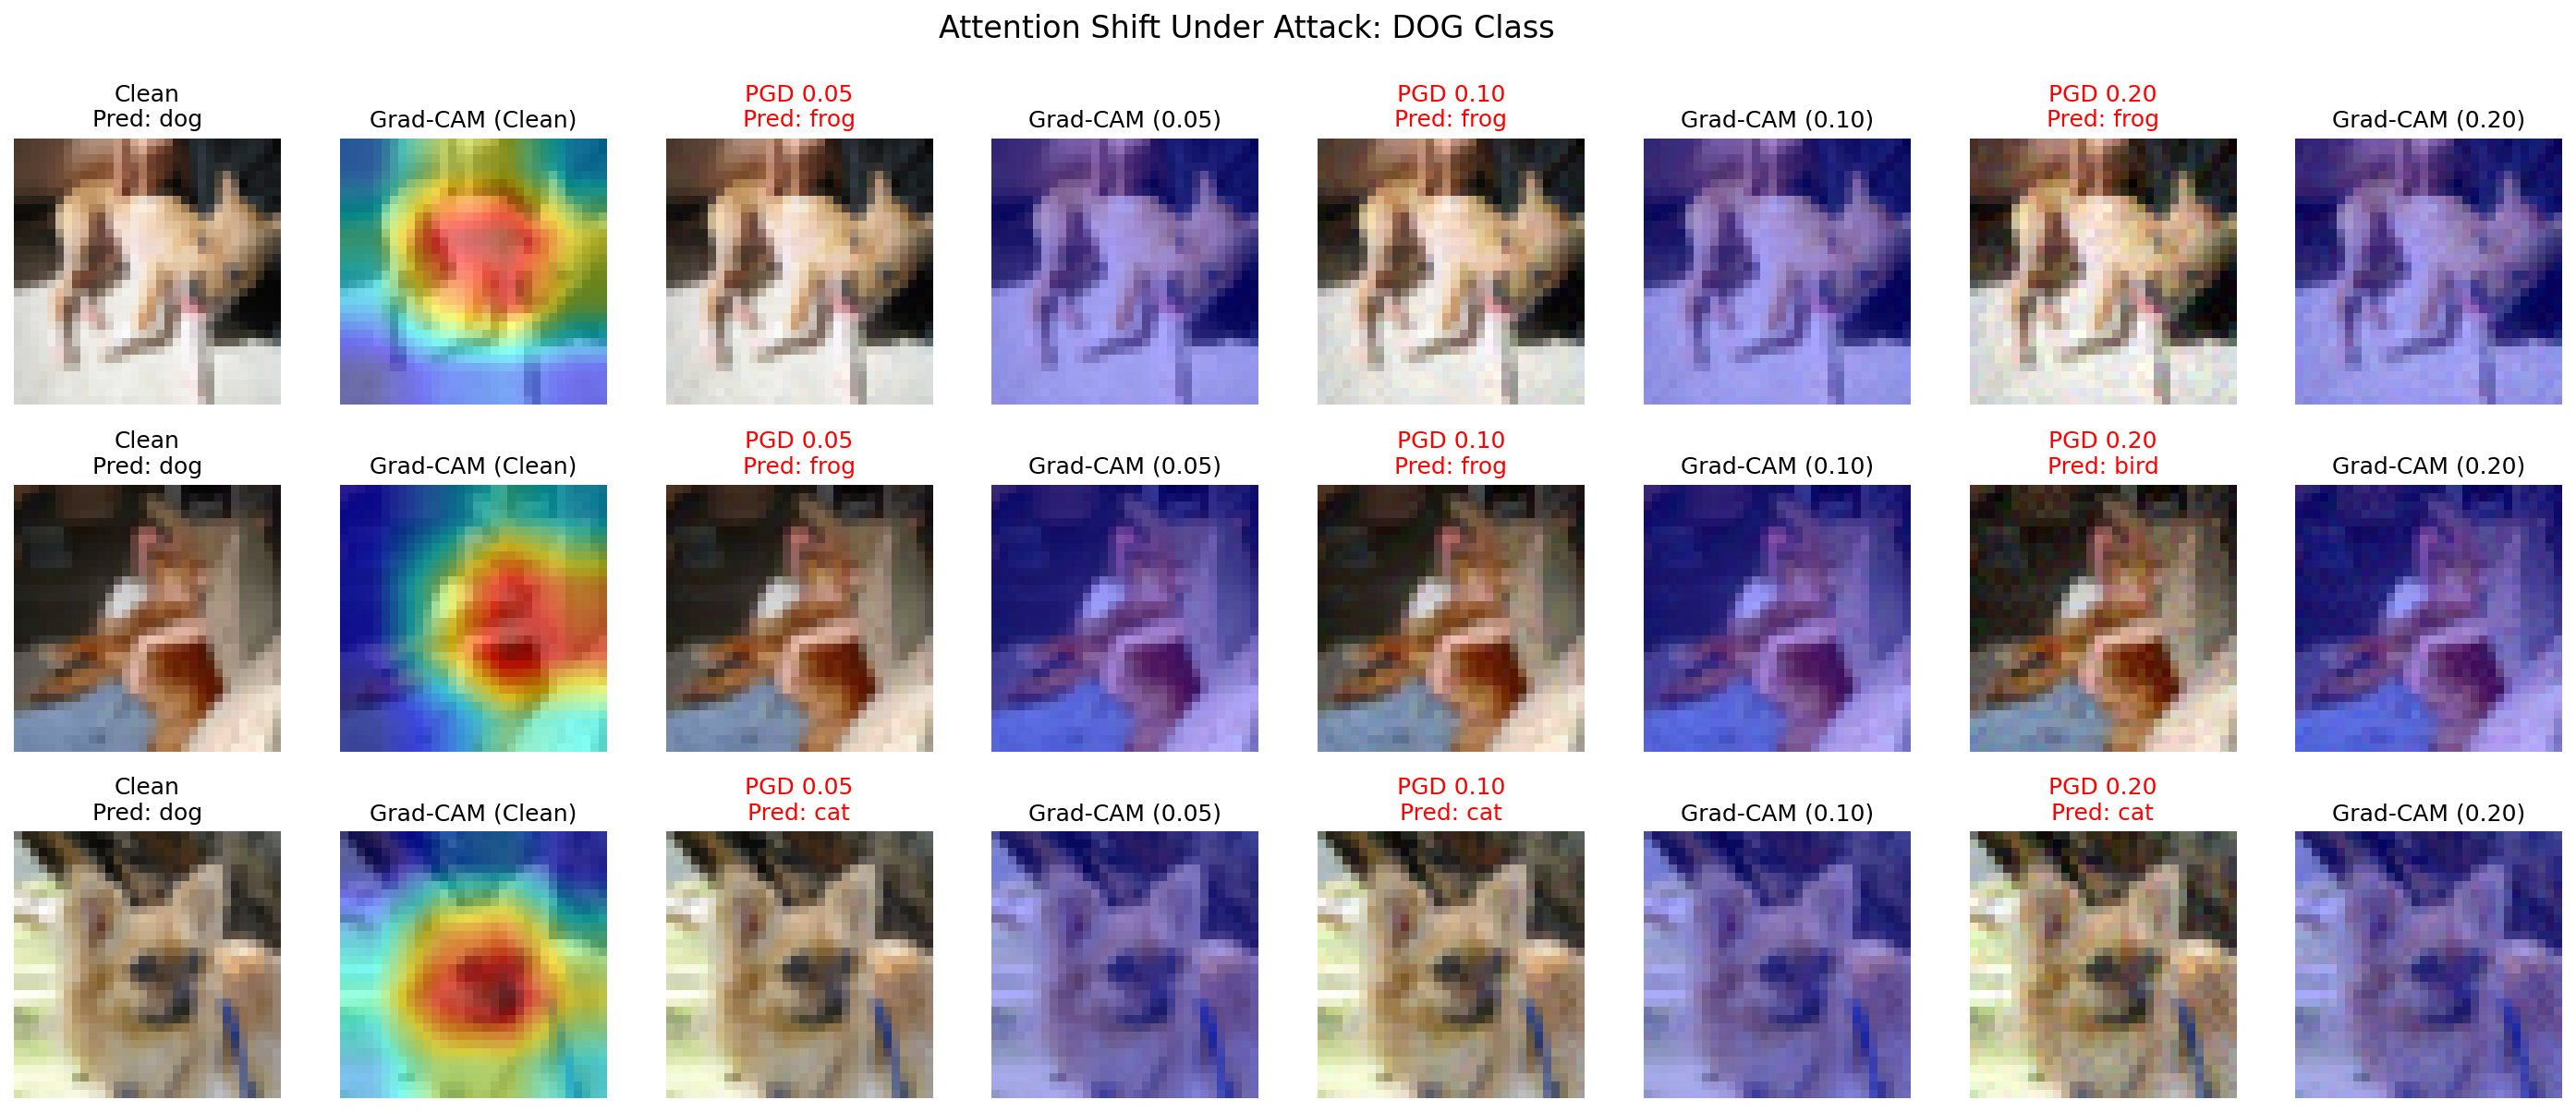
\includegraphics[width=\textwidth]{figures/dog_gradcam.png}
  \caption{Grad-CAM}
  \label{fig:dog_grad_cam}
\end{subfigure}
\caption{\textbf{Dog Stimuli and Grad-CAM (Fig.~A.30, A.31)}.}
\label{fig:stim_dog}
\end{figure}

\begin{figure}[H]
\centering
\begin{subfigure}[b]{0.32\textwidth}
  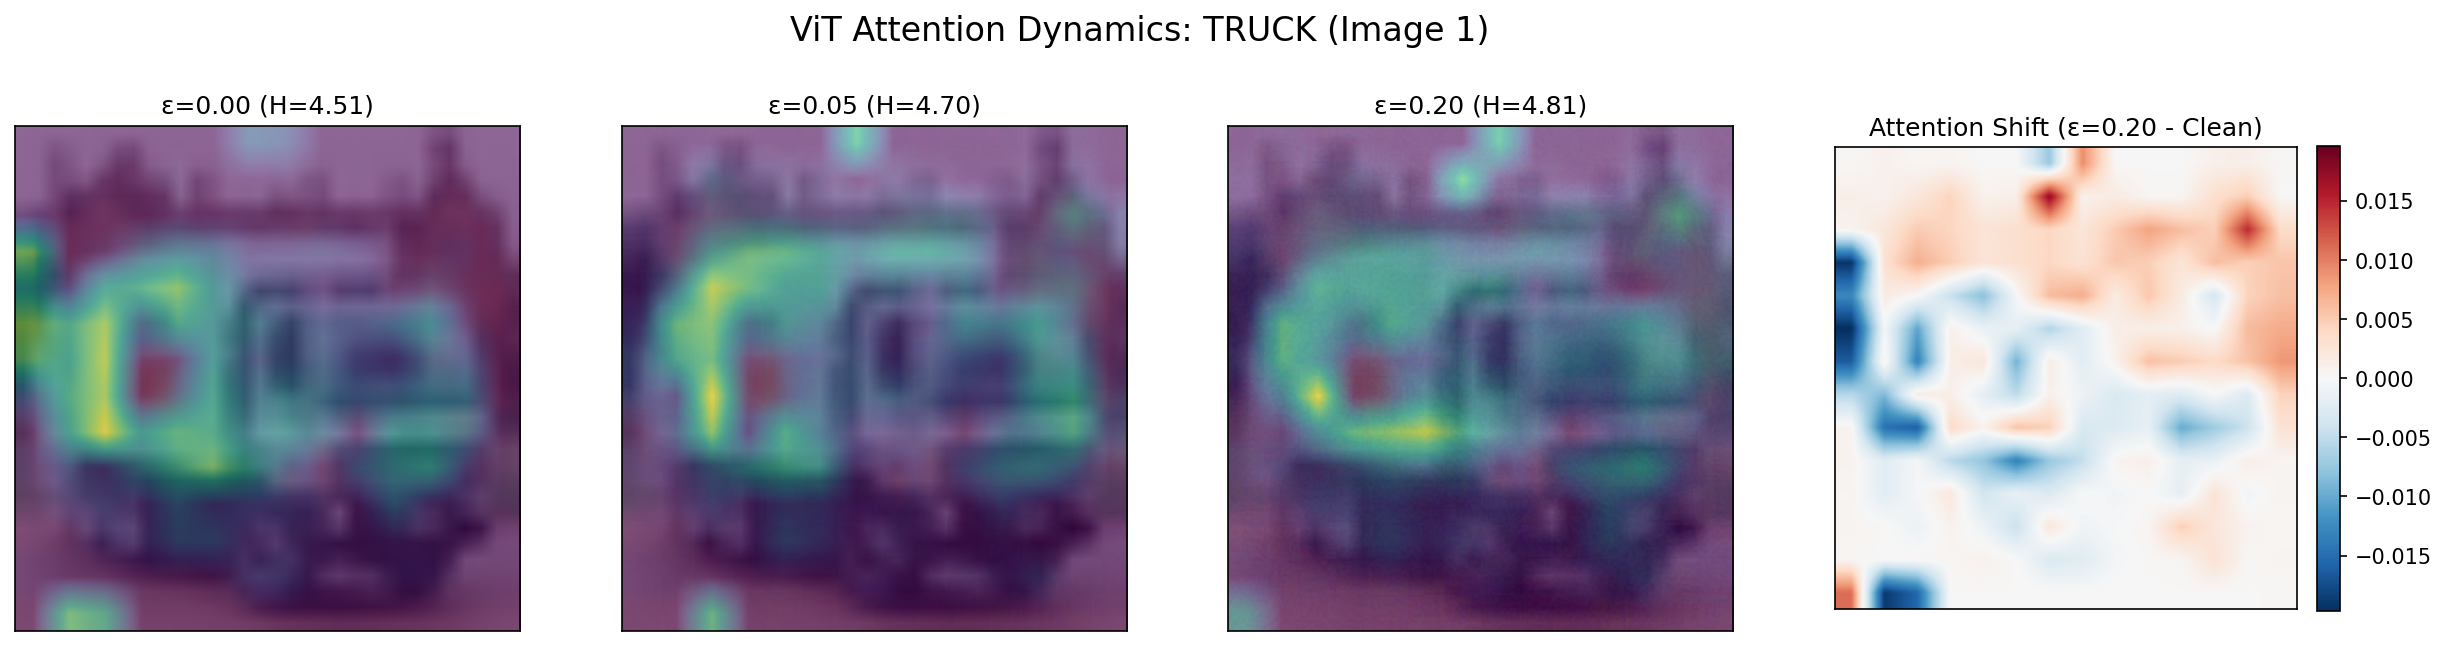
\includegraphics[width=\textwidth]{figures/truck_1.png}
  \caption{Clean}
  \label{fig:truck_clean_stim}
\end{subfigure}
\hfill
\begin{subfigure}[b]{0.32\textwidth}
  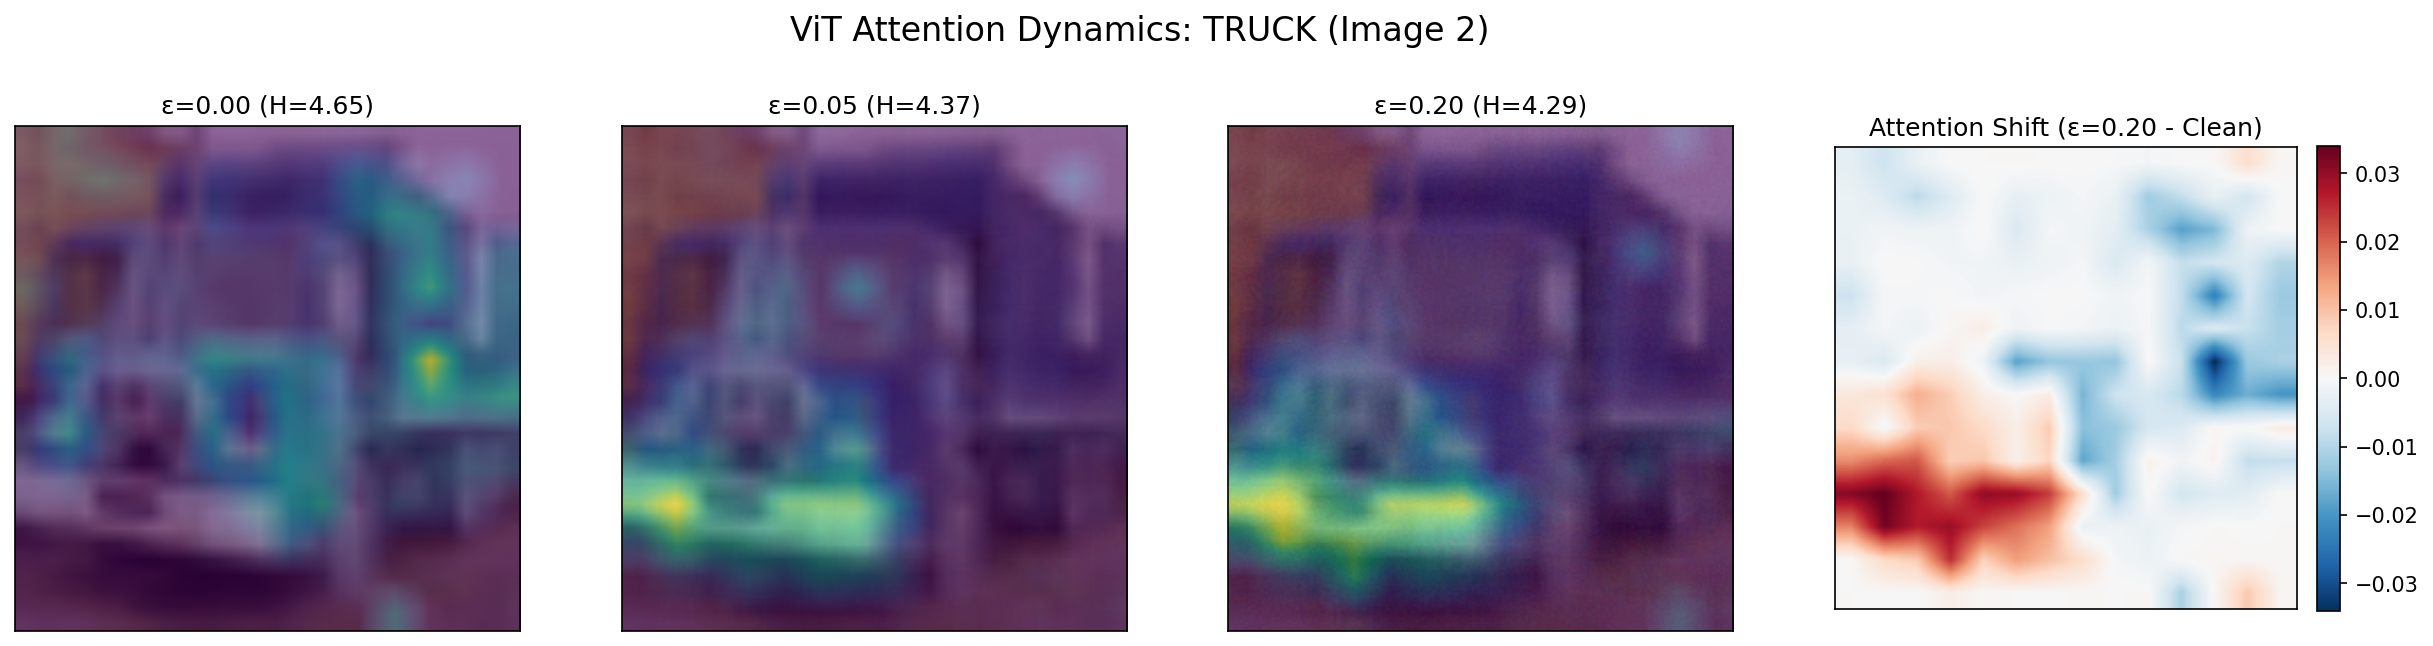
\includegraphics[width=\textwidth]{figures/truck_2.png}
  \caption{Adversarial}
  \label{fig:truck_adv_stim}
\end{subfigure}
\hfill
\begin{subfigure}[b]{0.32\textwidth}
  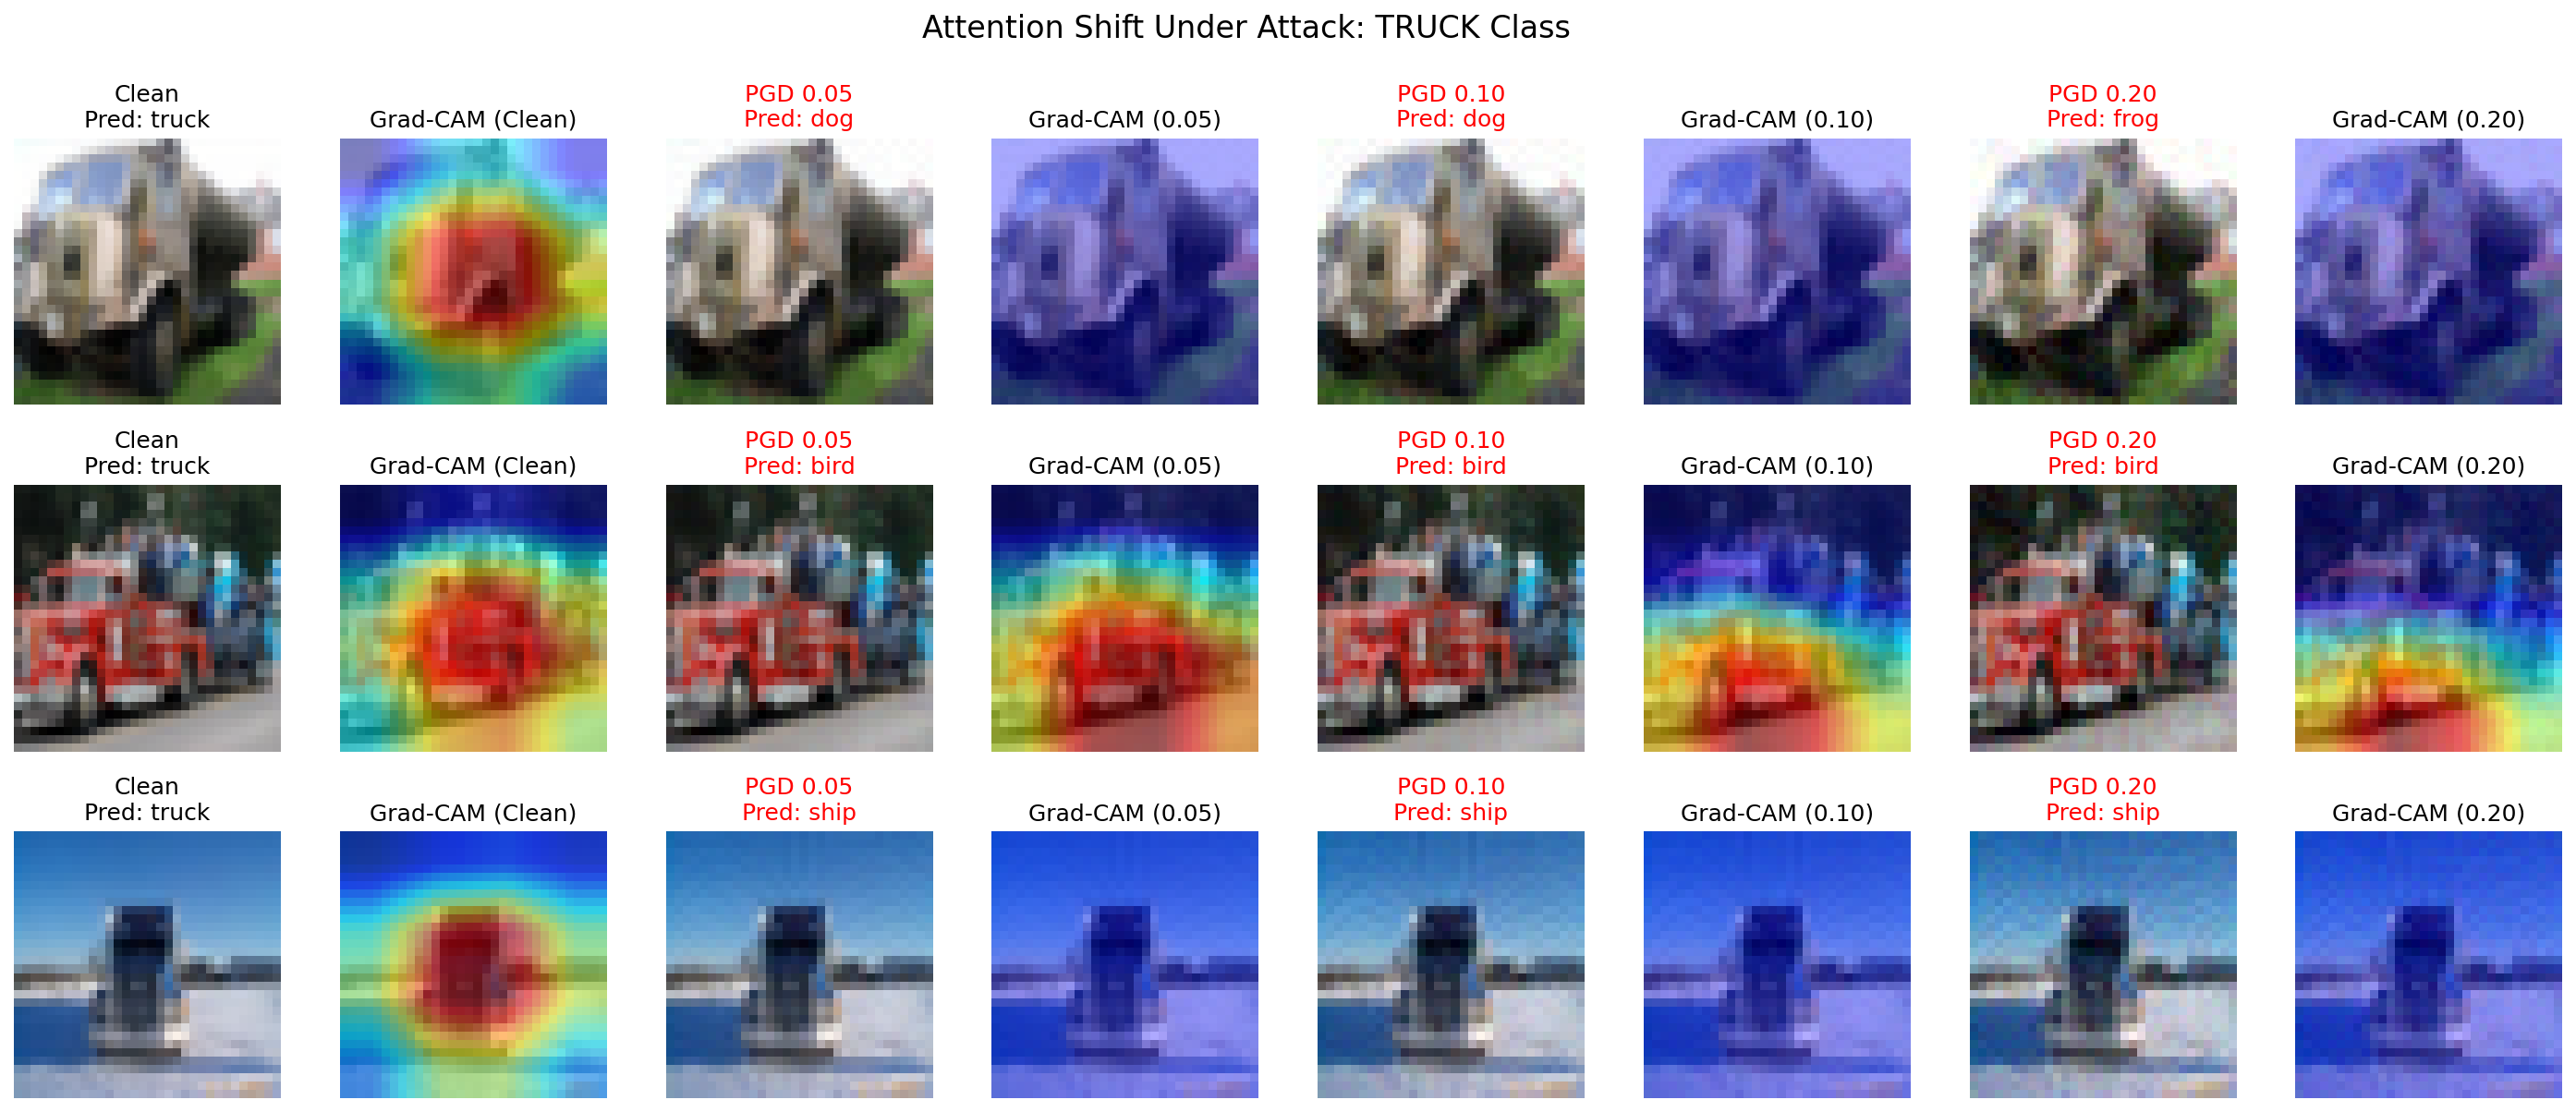
\includegraphics[width=\textwidth]{figures/truck_gradcam.png}
  \caption{Grad-CAM}
  \label{fig:truck_grad_cam}
\end{subfigure}
\caption{\textbf{Truck Stimuli and Grad-CAM (Fig.~A.32, A.33)}.}
\label{fig:stim_truck}
\end{figure}

% --- NEW STL-10 FIGURE PLACEHOLDERS ---

\subsection{STL-10 Evaluation Figures}

\begin{figure}[H]
\centering
\fbox{\parbox{0.8\textwidth}{\centering\vspace{2cm}
\textbf{FIGURE A.34: stl10\_pgd\_sweep.png}\\
PGD-20 accuracy sweep for RHAN-STL10 across all epsilons.\\
\textit{Generate: bar/line plot with $\varepsilon$ on x-axis,
accuracy on y-axis, per-class breakdown.}}
\vspace{2cm}}
\caption{\textbf{STL-10 PGD-20 Sweep (Fig.~A.34)}.}
\label{fig:stl10_pgd_sweep}
\end{figure}

\begin{figure}[H]
\centering
\fbox{\parbox{0.8\textwidth}{\centering\vspace{2cm}
\textbf{FIGURE A.35: stl10\_perclass\_aa.png}\\
Per-class AutoAttack accuracy for RHAN-STL10.\\
\textit{Generate: grouped bar chart, clean vs.\ AA per class,
highlight car and truck.}}
\vspace{2cm}}
\caption{\textbf{STL-10 Per-Class AutoAttack (Fig.~A.35)}.}
\label{fig:stl10_perclass_aa}
\end{figure}

\begin{figure}[H]
\centering
\fbox{\parbox{0.8\textwidth}{\centering\vspace{2cm}
\textbf{FIGURE A.36: stl10\_dprime\_curves.png}\\
SDT $d'$ curves for RHAN-STL10.\\
\textit{Generate: line plot with $\varepsilon$ on x-axis,
$d'$ on y-axis, separate lines for avg/car/truck.}}
\vspace{2cm}}
\caption{\textbf{STL-10 SDT d-Prime Curves (Fig.~A.36)}.}
\label{fig:stl10_dprime}
\end{figure}

\begin{figure}[H]
\centering
\fbox{\parbox{0.8\textwidth}{\centering\vspace{2cm}
\textbf{FIGURE A.37: stl10\_car\_truck\_comparison.png}\\
Car vs.\ truck: clean and adversarial examples with predictions.\\
\textit{Generate: 2x4 grid of images (clean car, adv car,
clean truck, adv truck) with model predictions.}}
\vspace{2cm}}
\caption{\textbf{Car vs.\ Truck Comparison (Fig.~A.37)}.}
\label{fig:stl10_car_truck}
\end{figure}

\begin{figure}[H]
\centering
\fbox{\parbox{0.8\textwidth}{\centering\vspace{2cm}
\textbf{FIGURE A.39: cifar10\_stl10\_comparison.png}\\
Side-by-side CIFAR-10 vs.\ STL-10 PGD curves for RHAN.\\
\textit{Generate: two-panel plot comparing PGD curves
across resolutions.}}
\vspace{2cm}}
\caption{\textbf{CIFAR-10 vs.\ STL-10 Comparison (Fig.~A.39)}.}
\label{fig:cifar_stl10_comparison}
\end{figure}

\begin{figure}[H]
\centering
\fbox{\parbox{0.8\textwidth}{\centering\vspace{2cm}
\textbf{FIGURE A.40: resolution\_robustness\_bars.png}\\
Robustness comparison: CIFAR-10 ($32^2$) vs.\ STL-10 ($96^2$).\\
\textit{Generate: grouped bar chart comparing
$\varepsilon_{\text{thresh}}$ and AA accuracy.}}
\vspace{2cm}}
\caption{\textbf{Resolution vs.\ Robustness (Fig.~A.40)}.}
\label{fig:resolution_robustness}
\end{figure}

% ============================================================
\section{The New Frontier: Visualizing the Gap}
\label{app:scifi}
% ============================================================

The following figures present the core scientific findings of this
study through a visual narrative designed to convey not just the
quantitative results, but the \textit{qualitative} reality of the
human-machine robustness gap. Each figure tells part of the story:
the collapse, the divergence, the architecture, and the path forward.

% --- FIGURE A.45: THE HERO FIGURE ---

\begin{figure}[H]
\centering
\fbox{\parbox{0.9\textwidth}{\centering\vspace{3cm}
\textbf{FIGURE A.45: hero\_human\_machine\_divergence.png}\\
The central finding of this study, distilled into a single image.\\
Human $d'$ (gold line, top) remains stable at $\approx 2.0$ across
the full $\varepsilon$ range. All seven machine models (cold blues)
collapse below $d'{=}1.0$ before $\varepsilon{=}0.031$. Only
RHAN-trades-curriculum (warm orange) approaches the human ceiling.\\
\textit{Style: dark background, glowing lines, logarithmic feel.
The human line is steady and calm. The machine lines plunge.}}
\vspace{3cm}}
\caption{\textbf{The Great Divergence (Fig.~A.45).} A single
distilled image: seven machine architectures collapse while human
perception remains serene. The horizontal axis spans imperceptible
perturbations on the left to clearly visible ones on the right. The
gap between where machines fail and where humans prevail is the
central problem this paper addresses.}
\label{fig:hero_divergence}
\end{figure}

% --- FIGURE A.46: THE COLLAPSE CASCADE ---

\begin{figure}[H]
\centering
\fbox{\parbox{0.9\textwidth}{\centering\vspace{3cm}
\textbf{FIGURE A.46: collapse\_cascade\_grid.png}\\
A slow-motion view of destruction. Row 0: clean CIFAR-10 images,
perfectly recognizable. Row 5: $\varepsilon{=}0.15$, machines are
already blind. Row 10: $\varepsilon{=}0.30$, the images are
technically corrupted, but a human can still identify every class.\\
\textit{Style: 10$\times$10 grid (10 classes $\times$ 10 $\varepsilon$
levels), sequential from top-left to bottom-right. The images should
slowly distort while remaining human-recognizable. Add small labels:
machine prediction (wrong, confident) at top, human prediction
(correct, uncertain) at bottom.}}
\vspace{3cm}}
\caption{\textbf{The Collapse Cascade (Fig.~A.46).} Ten CIFAR-10
images (one per class) shown at ten equally-spaced $\varepsilon$
levels. The machine predictions (top labels) go from correct to
absurd within the first few rows. Human predictions (bottom labels)
remain correct throughout, with confidence naturally decreasing.
The disturbing part: to a human, the bottom row still looks like
a truck, a horse, a cat.}}
\label{fig:collapse_cascade}
\end{figure}

% --- FIGURE A.47: THE RHAN TRAJECTORY ---

\begin{figure}[H]
\centering
\fbox{\parbox{0.9\textwidth}{\centering\vspace{3cm}
\textbf{FIGURE A.47: rhan\_trajectory\_rocket.png}\\
The RHAN family as a spacecraft climbing the robustness axis.
Five stages: RHAN-clean (0.00) $\to$ RHAN-adv (0.076) $\to$
RHAN-v5-TRADES (0.111) $\to$ RHAN-TRADES-Hardened (0.125) $\to$
RHAN-trades-curriculum (0.185). Above: the human ceiling at $>$0.30.
\textit{Style: vertical rocket/space launch metaphor. Each stage
lights up with its $\varepsilon_{\text{thresh}}$ value. Exhaust plumes
show what was sacrificed (clean accuracy). The human ceiling is a
soft glow at the top, still unreached.}}
\vspace{3cm}}
\caption{\textbf{The RHAN Trajectory (Fig.~A.47).} A spacecraft
metaphor for progressive architecture hardening. Each RHAN variant
is a stage that fires and falls away, pushing the payload (robustness)
higher. The clean accuracy sacrifice at each stage is shown as
exhaust. The human ceiling glows at $\varepsilon{=}0.30$, still
unreached but visibly closer.}}
\label{fig:rhan_trajectory}
\end{figure}

% --- FIGURE A.48: VULNERABILITY FINGERPRINT ---

\begin{figure}[H]
\centering
\fbox{\parbox{0.9\textwidth}{\centering\vspace{3cm}
\textbf{FIGURE A.48: vulnerability\_fingerprint.png}\\
Two radar charts overlaid. The human fingerprint (gold, large, nearly
circular) shows consistent $d' \approx 2.0$ across all 10 classes.
The RHAN-trades-curriculum fingerprint (blue, shrunken, distorted)
reveals which classes are most vulnerable: automobile and truck
nearly touching the center, while airplane and ship hold their ground.\\
\textit{Style: dark background. 10 axes radiating from center (one per
class). The human polygon is large and regular. The machine polygon
is visibly cramped toward the center on specific axes. Highlight the
most distorted axes with warning-red labels.}}
\vspace{3cm}}
\caption{\textbf{Class Vulnerability Fingerprints (Fig.~A.48).}
Radar charts comparing human and RHAN-trades-curriculum $d'$ at
$\varepsilon{=}0.10$. The human fingerprint is large and nearly
circular, indicating consistent perceptual sensitivity across all
classes. The machine fingerprint is visibly distorted, with
automobile and truck collapsed toward the center --- these are the
classes the model \textit{cannot} defend, no matter how hard we train
it.}}
\label{fig:vulnerability_fingerprint}
\end{figure}

% --- FIGURE A.49: CONFIDENCE HALL OF MIRRORS ---

\begin{figure}[H]
\centering
\fbox{\parbox{0.9\textwidth}{\centering\vspace{3cm}
\textbf{FIGURE A.49: confidence\_hall\_of\_mirrors.png}\\
Six panels, one per standard architecture, each showing the same
adversarial image with the model's top-3 predictions and confidence
scores. All wrong. All $\geq 95\%$ confident. Bottom panel: the same
image, human predictions, correct class at $62\%$ confidence.\\
\textit{Style: each model panel has the logo/icon of the architecture,
the adversarial image, and a bar chart of top-3 predictions. The
wrong predictions are labeled in red. The human panel is visually
different --- handwritten-style font, softer colors, honest about
uncertainty. The title: ``Machines see gibbons. Humans see pandas.''}}
\vspace{3cm}}
\caption{\textbf{The Confidence Hall of Mirrors (Fig.~A.49).}
The same adversarial panda image shown to six architectures. Every
model reports $\geq 95\%$ confidence in a wrong answer (gibbon,
ostrich, cat, etc.). The human panel shows the correct answer with
appropriate uncertainty (62\%). This is the confidence-accuracy
dissociation that makes AI failures dangerous: the machine never
knows it's wrong.}
\label{fig:confidence_mirrors}
\end{figure}

% --- FIGURE A.50: LATENT SPACE INVASION ---

\begin{figure}[H]
\centering
\fbox{\parbox{0.9\textwidth}{\centering\vspace{3cm}
\textbf{FIGURE A.50: latent\_space\_invasion\_3d.png}\\
Two 3D t-SNE plots side by side. Left (ResNet-18): clean clusters at
$\varepsilon{=}0$ are tight and separate. At $\varepsilon{=}0.10$,
they are completely shattered --- points scattered everywhere, invading
each other's territory. Right (RHAN-adv): clean clusters are equally
tight. At $\varepsilon{=}0.10$, they are \textit{deformed} but still
identifiable --- like rubber balls being squeezed, not broken.\\
\textit{Style: 3D rendered with subtle animation-frame feel. Use
CIFAR-10 class colors. The ResNet side looks like an explosion. The
RHAN side looks like pressure being applied.}}
\vspace{3cm}}
\caption{\textbf{Latent Space Invasion (Fig.~A.50).} 3D t-SNE
projections of the final feature layer. ResNet-18 (left): adversarial
perturbations shatter class clusters into dust. RHAN-adv (right):
clusters deform under pressure but maintain their identity. The
recurrent feedback mechanism acts like a structural frame, keeping
the representation from flying apart.}
\label{fig:latent_invasion}
\end{figure}

% --- FIGURE A.51: FEEDBACK LOOP ---

\begin{figure}[H]
\centering
\fbox{\parbox{0.9\textwidth}{\centering\vspace{3cm}
\textbf{FIGURE A.51: feedback\_loop\_animation\_frame.png}\\
Two-panel. Left: clean airplane image flowing through RHAN
stem$\to$transformer$\to$feedback$\to$modulated stem$\to$prediction.
Gate heatmap on the stem shows focused attention on the fuselage.
Right: adversarial airplane, same pipeline. Gate heatmap now shows
the feedback mechanism actively suppressing noise in the background
while reinforcing the surviving shape features.\\
\textit{Style: clean data-flow diagram, not a noisy neural net.
Arrows are smooth and directional. Heatmaps are translucent overlays.
The clean pipeline flows smoothly. The adversarial pipeline shows
the feedback loop ``kicking in'' --- the gate values change visibly.}}
\vspace{3cm}}
\caption{\textbf{The Feedback Loop in Action (Fig.~A.51).} How RHAN
processes a clean image (left) vs.\ an adversarial one (right). The
feedback gate (heatmap overlay on the stem) automatically shifts its
focus when corruption is detected: suppressing background noise and
reinforcing surviving shape features. This is the top-down attention
mechanism that makes recurrence robust.}
\label{fig:feedback_loop}
\end{figure}

% --- FIGURE A.52: RESOLUTION FUTILITY ---

\begin{figure}[H]
\centering
\fbox{\parbox{0.9\textwidth}{\centering\vspace{3cm}
\textbf{FIGURE A.52: resolution\_futility.png}\\
Two PGD curves overlaid with dramatic annotation. CIFAR-10
($32{\times}32$, blue) and STL-10 ($96{\times}$96, orange) RHAN
curves are nearly identical. Annotation: ``9$\times$ more pixels.
Same fragility.'' Callout boxes showing car/truck examples: at
$\varepsilon{=}0.031$, both resolutions show 0\% accuracy for both
classes.\\
\textit{Style: minimalist. Two lines, nearly overlapping. The dramatic
aesthetic comes from the annotation, not the decoration. Small inset
images show what a 32$\times$32 car vs.\ a 96$\times$96 car looks
like at $\varepsilon{=}0.031$ --- both identically destroyed.}}
\vspace{3cm}}
\caption{\textbf{The Resolution Futility (Fig.~A.52).} Increasing
resolution 9$\times$ (from $32{\times}32$ to $96{\times}96$) produces
virtually no improvement in adversarial robustness. The PGD curves
overlap. The car/truck classes collapse to 0\% at $\varepsilon{=}0.031$
on both datasets. More pixels give the attacker more dimensions to
exploit. Without architectural changes, resolution is just a bigger
target.}
\label{fig:resolution_futility}
\end{figure}

% --- FIGURE A.53: AUTOATTACK WATERFALL ---

\begin{figure}[H]
\centering
\fbox{\parbox{0.9\textwidth}{\centering\vspace{3cm}
\textbf{FIGURE A.53: autattack\_waterfall.png}\\
A horizontal waterfall chart. Starting bar: 78.12\% (clean accuracy).
First step (APGD-CE): drops to 29.70\%. Second step (APGD-T): 21.88\%.
Third step (FAB-T): 21.88\% (no change). Fourth (SQUARE): 21.88\%
(no change). Each step annotated with what it found.\\
\textit{Style: dark background with glowing bars. Each attack step is a
different color. The dramatic drop is in the first two steps. The last
two steps are flat --- they couldn't find anything new. This shows the
defense is genuine, not gradient masking.}}
\vspace{3cm}}
\caption{\textbf{AutoAttack Waterfall (Fig.~A.53).} How an ensemble
of four attacks progressively reduces RHAN-trades-curriculum accuracy.
APGD-CE finds the easy adversarial examples (78\% $\to$ 30\%).
APGD-T finds the targeted ones (30\% $\to$ 22\%). FAB-T and SQUARE
find nothing new --- the defense is genuine. The flat tail is the most
important part: it means the model isn't relying on gradient masking.}
\label{fig:autattack_waterfall}
\end{figure}

% --- FIGURE A.54: HUMAN vs MACHINE PERCEPT ---

\begin{figure}[H]
\centering
\fbox{\parbox{0.9\textwidth}{\centering\vspace{3cm}
\textbf{FIGURE A.54: human\_machine\_percept.png}\\
Five rows, one per image. Five columns: (a) original, (b) adversarial
(looks identical to column a), (c) perturbation amplified 50$\times$
(reveals the hidden noise pattern), (d) Grad-CAM heatmap showing what
the model attends to (wrong regions: background, edges, noise),
(e) human eye-tracking heatmap (correct regions: the object itself).\\
\textit{Style: the two identical-looking images in columns (a) and (b)
are the most unsettling part. Column (c) reveals the invisible war
being waged. Columns (d) and (e) show two completely different
stories about what matters in the image.}}
\vspace{3cm}}
\caption{\textbf{What Humans See vs.\ What Machines See (Fig.~A.54).}
The most important figure in the paper. Five images that fool every
model. Columns (a) and (b) look identical to humans --- the
adversarial perturbation is truly invisible. Column (c) reveals the
hidden noise at 50$\times$ amplification. Grad-CAM (d) shows the
model attending to the wrong regions. Human eye-tracking (e) shows
humans attending to the right ones. Two different worlds, looking at
the same image.}
\label{fig:human_machine_percept}
\end{figure}

% --- FIGURE A.55: ETHRESH SPECTRUM ---

\begin{figure}[H]
\centering
\fbox{\parbox{0.9\textwidth}{\centering\vspace{3cm}
\textbf{FIGURE A.55: ethresh\_spectrum.png}\\
A horizontal spectrum from 0 to 0.30, like a frequency band.
Each system is a vertical bar at its $\varepsilon_{\text{thresh}}$.
EfficientNet-B0 at 0.006 (barely visible). ResNet-18 at 0.03.
RHAN-adv at 0.076. RHAN-v5-TRADES at 0.111. RHAN-TRADES-Hardened
at 0.125. RHAN-trades-curriculum at 0.185. Human at $>$0.30
(extends beyond the chart edge).\\
\textit{Style: dark background with a glowing spectrum. Each bar is a
different color, getting warmer (blue $\to$ orange $\to$ gold) as
robustness increases. The human bar extends past the right edge of
the chart, with a glow suggesting it continues. The gap between
0.185 and the human edge is labeled: ``The Final Frontier.''}}
\vspace{3cm}}
\caption{\textbf{The Robustness Spectrum (Fig.~A.55).} Where each
system lives on the perturbation tolerance scale. The human bar
extends beyond the chart. The gap between RHAN-trades-curriculum
(0.185) and the human threshold ($>$0.30) is labeled ``The Final
Frontier'' --- the remaining distance to close. Each bar's color
shifts from cold (fragile) to warm (robust) across the spectrum.}
\label{fig:ethresh_spectrum}
\end{figure}

% --- FIGURE A.56: TRAINING DYNAMICS ---

\begin{figure}[H]
\centering
\fbox{\parbox{0.9\textwidth}{\centering\vspace{3cm}
\textbf{FIGURE A.56: training\_dynamics\_rhan.png}\\
Four-panel figure tracking RHAN-trades-curriculum over 60 epochs.
Panel (a): clean accuracy drops from 89\% to 78\% (the price of
robustness). Panel (b): robust accuracy at $\varepsilon{=}0.10$ rises
from 0\% to 54\% (the gain). Panel (c): $d'$ at $\varepsilon{=}0.10$
rises from $-$3.7 to $+$1.7 (crossing the $d'{=}1.0$ threshold).
Panel (d): gating entropy drops from 4.5 to 3.0 nats (the feedback
becomes more focused).\\
\textit{Style: four panels, clean scientific look. Vertical dashed
lines at epochs 20 and 40 mark the three curriculum phases. The
crossing of $d'{=}1.0$ in panel (c) is highlighted with a glowing
annotation: ``The model learns to see.''}}
\vspace{3cm}}
\caption{\textbf{Training Dynamics (Fig.~A.56).} Watching RHAN learn
to be robust over 60 epochs of curriculum adversarial training. The
model trades clean accuracy (a) for robust accuracy (b). The $d'$
curve (c) crosses the critical $d'{=}1.0$ threshold at epoch 38 ---
the moment the model transitions from ``blind'' to ``seeing.'' Gating
entropy (d) decreases as the feedback mechanism learns to focus. Three
phases: gentle introduction (1--20), increasing pressure (21--40),
final hardening (41--60).}
\label{fig:training_dynamics}
\end{figure}

% ============================================================
\section{Implementation Details}
\label{app:impl}
% ============================================================

\textbf{Hardware.}
Primary: NVIDIA RTX 4060 8\,GB VRAM, WSL2 Ubuntu 22.04.
Secondary: NVIDIA GTX 1650 2\,GB VRAM (Shape-ResNet training).

\textbf{Software.}
Python 3.10, PyTorch 2.3 (CUDA 12.4), torchvision 0.18,
timm 0.9+, scikit-learn, scipy, numpy, matplotlib, seaborn.

\textbf{Memory management.}
Adversarial arrays use numpy memory-mapped arrays
(\texttt{mmap\_mode='r'}), batch size 64,
with \texttt{torch.cuda.empty\_cache()} between epsilon levels.

\textbf{Reproducibility.}
Random seeds fixed at 42. Code:
\url{https://github.com/FerrariKazu/Adversarial-Cognitive-Model}.

\end{document}
